\documentclass[12pt,a4paper]{article}
\usepackage[utf8]{inputenc}
\usepackage[english]{babel}
\usepackage[english]{isodate}
\usepackage[parfill]{parskip}
\usepackage{graphicx}
\usepackage{natbib}
\usepackage{hyperref}
\usepackage{amsmath}
\usepackage{amssymb}
\usepackage{multirow}
\usepackage{float}
\usepackage{rotating}
\usepackage{array}
\usepackage[dvipsnames]{xcolor}

%opening

\title{\begin{figure}[H]%figure01a
\centerline{
\includegraphics[]{PhenStat_logo.png}}
\end{figure}\textbf{PhenStat}: \\ statistical analysis of phenotypic data\\ \textbf{User's Guide}}
\author{Natalja Kurbatova, Natasha Karp, Jeremy Mason}
\date{Last revised: \today}

\begin{document}
\maketitle
\newpage
\tableofcontents
\newpage
\section{Introduction}
High-throughput phenotyping generates large volumes of varied data including both categorical and continuous data. Operational and cost constraints can lead to a work-flow that precludes traditional analysis methods. Furthermore, for a high throughput environment, a robust automated statistical pipeline that alleviates manual intervention is required. 

PhenStat is a package that provides statistical methods for the identification of abnormal phenotypes with an emphasize on high-throughput data-flows. The package contains dataset checks and cleaning in preparation for the analysis, four statistical frameworks for the phenodeviants identification and additional functions that help to decide the correct method for analysis. 

Simple explanation of statistical frameworks is given below. More details can be found in the appropriate sections of the User's Guide. 

We also have implemented the \href{http://www.bioconductor.org/packages/bioc/html/IMPCdata.html}{IMPCdata package}  that allows easy access to the phenotyping data produced by the International Mouse Phenotyping Consortium (IMPC) and is available in Bioconductor.
%For continuous data, an iterative fitting process is used to fit a regression model that is the most appropriate for the data (Mixed Model framework), whilst for categorical data, a Fisher Exact Test is implemented (Fisher Exact Test framework). In addition, the reference range method (Reference Range Plus framework) is added into the package as a conservative method of identifying phenodeviants.

\begin{enumerate}
\item Mixed Models framework assumes that base line values of dependent variable are normally distributed but batch (assay date) adds noise and models variables accordingly in order to separate the batch and the genotype. 
Model optimisation starting with:

$depVariable=Genotype+Sex+Genotype*Sex + Weight + (1|Batch)$

Assume batch is normally distributed with defined variance. This framework can be used in case when you have controls measured over multiple batches and you ideally have knockout mice measured in multiple batches. The knockouts do not have to be concurrent with controls.
\begin{figure}[H]%figure01a
\centerline{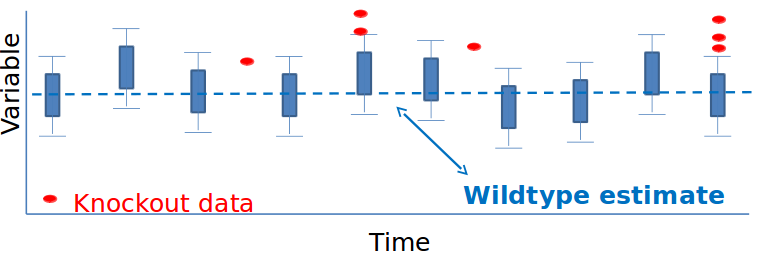
\includegraphics[scale=0.4]{MM_simple.png}}
\end{figure}

\item Time Fixed Effect framework estimates each batch effect to separate it from genotype.
Model optimisation starting with:

$depVariable=Genotype+Sex+Genotype*Sex + Weight + Batch$

This framework can be used in case when there are up to 5 batches and concurrent controls approach had been used. 
\begin{figure}[H]%figure01a
\centerline{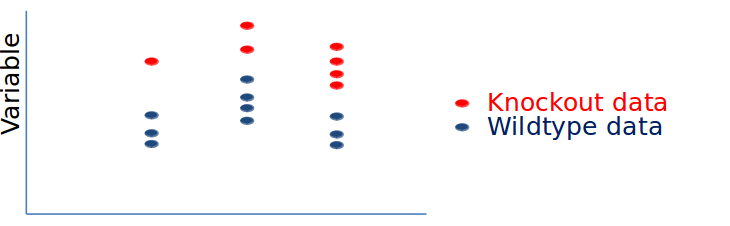
\includegraphics[scale=0.4]{TFE_simple.png}}
\end{figure}

\item Reference Range Plus framework identifies the normal variation form the wildtype animals, classifies dependent variables from the genotype of interest as low, normal or high and compares proportions to assess for movement towards high or low class borders.  
\begin{figure}[H]%figure01a
\centerline{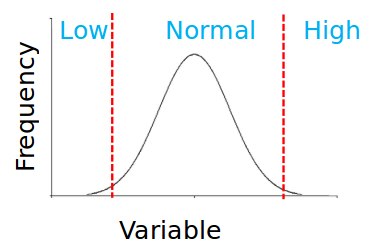
\includegraphics[scale=0.4]{RR1_simple.png}}
\end{figure} 
\begin{figure}[H]%figure01a
\centerline{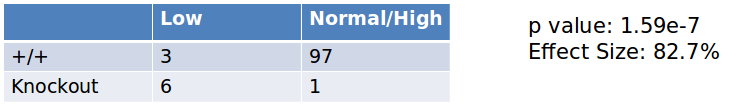
\includegraphics[scale=0.4]{RR2_1_simple.png}}
\end{figure}
\begin{figure}[H]%figure01a
\centerline{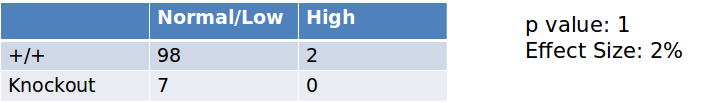
\includegraphics[scale=0.4]{RR2_2_simple.png}}
\end{figure}

This framework requires sufficient number of controls (more than 60 records) in order to correctly identify normal variation and can be used when other methods are not applicable or as a first simple data assessment method. 
\item Fisher Exact Test is a standard framework for categorical data which compares data proportions and calculates the percentage change in classification.
\begin{figure}[H]%figure01a
\centerline{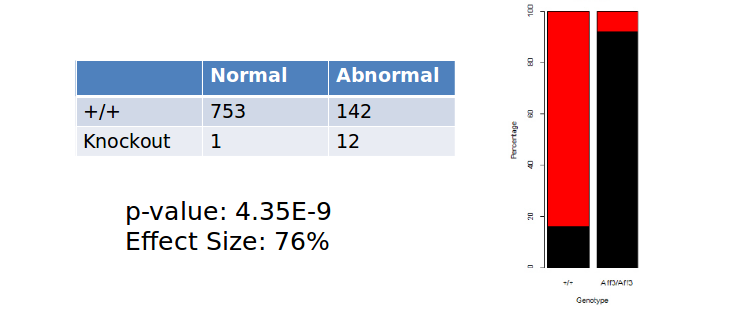
\includegraphics[scale=0.4]{FE_simple.png}}
\end{figure}

\item Logistic Regression is a framework for categorical data recoded to two levels: 0 (e.g. as expected or reference phenotype) and 1 (abnormal). This method models the relationship between the variable of interest and a number of independent variables assessing the impact of sex, genotype and whether the genotype effect depends on the sex.
\begin{figure}[H]%figure01a
\centerline{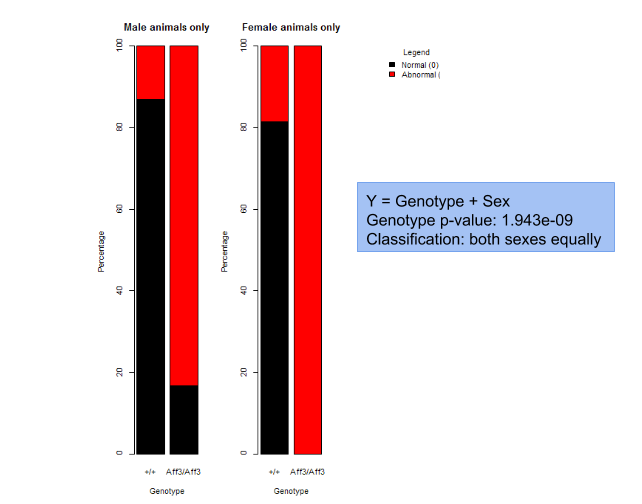
\includegraphics[scale=0.5]{LR_simple.png}}
\end{figure}

\end{enumerate}

All analysis frameworks output a statistical significance measure, an effect size measure, model diagnostics (when appropriate), and graphical visualisation of the genotype effect. 

Depending on the user needs, the statistical analysis output can either be interactive where the user can view the graphical output and analysis summary or for a database implementation the output consists of a vector of output and saved graphical files. 

This package has been tested and demonstrated with an application of 420 lines of historic mouse phenotyping data from the  \href{http://www.sanger.ac.uk/mouseportal/}{Sanger MGP} and \href{http://www.europhenome.org/}{Europhenome} resources. Please note, the testing of the Time Fixed Effect framework has been limited due to the shortage of suitable datasets.
\\

\begin{figure}[!htpb]%figure01
\centerline{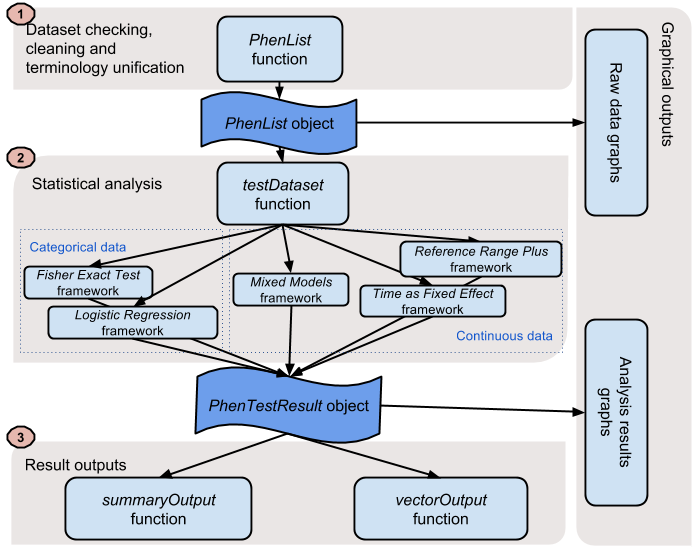
\includegraphics[scale=0.5]{PhenStat_simple.png}}
\caption{The PhenStat package's three stage structure: dataset processing, statistical analysis, and result output.}\label{fig:01}
\end{figure}

The package consists of three stages as shown in Figure \ref{fig:01}:
\begin{enumerate}
\item Dataset processing: includes checking, cleaning and terminology unification procedures and is completed by function \textit{PhenList} which creates a \textit{PhenList} object. 
\item Statistical analysis: is managed by function \textit{testDataset} and consists of Mixed Model, Time Fixed Effect, Reference Range Plus, Fisher Exact framework and Logistic Regression framework implementations. The results are stored in \textit{PhenTestResult} object. 
Potentially this layer can be extended adding new statistical methods. 
\item Results Output: depending on user needs there are two functions for the test results output: \textit{summaryOutput} 
and \textit{vectorOutput} that present data from \textit{PhenTestResult} object in a particular format. The output layer is also easily extendible.
\end{enumerate}

Package has a function \textit{recommendMethod} to assess the suitability of the dataset for the various statistical analysis methods.
 
Package run time depends on a variety of factors including dataset size, computational resources, etc. Average analysis \textbf{run time} of the pilot dataset in our local environement is \textbf{1.34 seconds}. 


\section{Data Processing with PhenList Function}
\textit{PhenList} function performs data processing and creates a \textit{PhenList} object. 
As input, \textit{PhenList} function requires dataset of phenotypic data that can be presented as data frame. For instance, it can be dataset stored in csv or txt file. 


\begingroup
    \fontsize{8pt}{12pt}\selectfont
\begin{verbatim}
> dataset <- read.csv("myPhenotypicDataset.csv")
> dataset <- read.table("myPhenotypicDataset.txt",sep="\t")
\end{verbatim}
\endgroup
Data is organised with a row for a sample and each column provides information such as meta data (strain, genotype, etc.) and the variable of interest.

In Table \ref{table:01} the example dataset is presented with numerical variables of interest. Table \ref{table:02} shows the example dataset with categorical data. 

In addition to dependent variable column (the variable of interest) mandatory columns are "Genotype" and "Sex". The "Assay.Date" column is used to model "Batch" effect if not specified differently. "Weight" column is used to model body weight effect.

The information provided in the "Assay.Date" column is treated as a categorical variable with different strings as different levels.  As such there is no requirement to provide the date in any particular format (ie D\textbackslash M\textbackslash Y or M\textbackslash D\textbackslash Y) however please remove any time stamp.  Removing the time stamp is necessary such that data will cluster by day appropriately.
\begin{sidewaystable}
 \begin{tabular}{| p{13mm} | p{13mm} | l | l | l | p{19mm}| p{12mm} | l | p{13mm} | p{12mm} | p{12mm} | l |}
  \hline
Colony.\newline Prefix&Gene.\newline Name&Mouse&\textbf{Genotype}&\textbf{Sex}&\textbf{Assay.\newline Date}&Age.In.\newline Weeks&\textbf{Weight}&Bone\newline Mineral.\newline Density&Bone.\newline Area&Lean.\newline Mass& ... \\\hline
MBAU&Sparc&M00260466&Sparc/Sparc&Female&07-Aug-09&13.7&26.7&0.0443&8.46&17.29&\\
MBAU&Sparc&M00260467&Sparc/Sparc&Female&07-Aug-09&13.7&27.6&0.0427&7.95&15.99&\\
MBAU&Sparc&M00260468&Sparc/Sparc&Female&07-Aug-09&13.7&30.7&0.0451&8.95&17.73&\\
MBAU&Sparc&M00260475&Sparc/Sparc&Female&07-Aug-09&14.3&24.9&0.0443&8.43&14.84&\\
MBAU&Sparc&M00330799&Sparc/Sparc&Female&23-Nov-09&14&27.9&0.047&8.79&17.34&\\
MBAU&Sparc&M00330800&Sparc/Sparc&Female&23-Nov-09&14&25.1&0.0433&8.52&15.84&\\
MBAU&Sparc&M00330801&Sparc/Sparc&Female&23-Nov-09&14&21.7&0.0419&7.46&15.38&\\
MBAU&Sparc&M00226962&Sparc/Sparc&Male&23-Jun-09&13.9&32.8&0.0454&9.73&18.31&\\
MBAU&Sparc&M00226963&Sparc/Sparc&Male&23-Jun-09&13.9&38&&&&\\
MBAU&Sparc&M00226964&Sparc/Sparc&Male&23-Jun-09&13.9&34.9&0.0471&11&19.64&\\
MBAU&Sparc&M00354835&Sparc/Sparc&Male&06-Jan-10&14.1&38.5&0.0483&10.28&21.91&\\
MBAU&Sparc&M00354836&Sparc/Sparc&Male&06-Jan-10&14.1&35.8&0.0486&9.65&20.8&\\
MBAU&Sparc&M00354837&Sparc/Sparc&Male&06-Jan-10&14.1&40.6&0.0483&10.08&24.25&\\
MBAU&Sparc&M00405764&Sparc/Sparc&Male&01-Mar-10&14&35.1&0.0465&9.25&20.25&\\
MBAU&Sparc&M00405766&Sparc/Sparc&Male&01-Mar-10&14&33.2&0.0465&10.17&19.54&\\
MBAU&Sparc&M00405767&Sparc/Sparc&Male&01-Mar-10&14&32.6&0.0444&8.88&20.07&\\
MALA&Ccdc57&M00194360&+/+&Female&05-May-09&14.3&23.9&0.0461&8.75&18.93&\\
MAOA&Yipf1&M00191904&+/+&Female&07-May-09&14&33.8&0.0512&8.8&19.71&\\
MAOA&Yipf1&M00191913&+/+&Female&07-May-09&14.3&29&0.0519&9.69&18.66&\\
MBFD&Gatc&M00191104&+/+&Female&08-May-09&14.1&26.5&0.0502&8.8&18.37&\\
MBFD&Gatc&M00191105&+/+&Female&08-May-09&14.1&40.7&0.0529&10.42&21.71&\\
MBFD&Gatc&M00195130&+/+&Female&08-May-09&13.1&26.1&0.0474&8.84&19.41&\\
MBFD&Gatc&M00191134&+/+&Female&08-May-09&13.9&33.1&0.0501&10.03&18.33&\\
MBHU&Mgst3&M00197544&+/+&Female&14-May-09&13.9&30.5&0.0477&9.08&17.92&\\
MBHU&Mgst3&M00197565&+/+&Female&14-May-09&14&34&0.0514&8.91&19.12&\\
MBHU&Mgst3&M00197566&+/+&Female&14-May-09&14&31.9&0.0496&9.01&18.17&\\
MBHU&Mgst3&M00197567&+/+&Female&14-May-09&14&35.6&0.0524&9.94&19.46&\\
MBRR&Myo5a&M00197538&+/+&Female&15-May-09&14&32.7&0.0503&9.27&19.12&\\
MAIT&Setdb1&M00195664&+/+&Female&18-May-09&14.1&31.2&0.0468&8.51&17.67&\\
...&...&...&...&...&...&...&...&...&...&...&\\
\hline  
\end{tabular}
\caption{The continuous dataset example.}\label{table:01}
\end{sidewaystable}

\begin{sidewaystable}
\begin{tabular}{| p{13mm} | p{15mm} | l | l | l | p{19mm}| p{12mm} |  p{16mm}  | p{17mm} | p{16mm} | p{17mm} | l |}
  \hline
Colony.\newline Prefix&Gene.\newline Name&Mouse&\textbf{Genotype}&\textbf{Sex}&\textbf{Assay.\newline Date}&Age.In.\newline Weeks&Caudal.\newline Processes&Cervical.\newline Processes&Lumbar.\newline Processes&Thoracic.\newline Processes& ... \\\hline
MAPP&Smarcal1&M01005699&+/+&Male&12-Mar-12&13.9&Normal&Abnormal&Normal&Normal&\\
MCUB&Egfr&M01114643&+/+&Male&04-Jul-12&13.9&Normal&Normal&Normal&Normal&\\
MDYA&Srrm4&M01108371&+/+&Female&04-Jul-12&13.9&Normal&Abnormal&Normal&Normal&\\
MDYA&Srrm4&M01108373&+/+&Female&04-Jul-12&13.9&Normal&Normal&Normal&Normal&\\
MEFV&Gpr107&M01167360&+/+&Male&04-Sep-12&14&Normal&Abnormal&Normal&Normal&\\
MEFV&Gpr107&M01167394&+/+&Male&04-Sep-12&14&Normal&Abnormal&Normal&Normal&\\
MEFV&Gpr107&M01167391&+/+&Male&04-Sep-12&14&Normal&Abnormal&Normal&Normal&\\
MEFV&Gpr107&M01167363&+/+&Female&04-Sep-12&14&Normal&Abnormal&Normal&Abnormal&\\
MDYQ&Fam175b&M01128905&+/+&Female&17-Jul-12&13.9&Normal&Abnormal&Normal&Normal&\\
MDYQ&Fam175b&M01128906&+/+&Female&17-Jul-12&13.9&Normal&Abnormal&Normal&Normal&\\
MEGD&Slitrk4&M01140446&+/+&Male&06-Aug-12&14&Normal&Abnormal&Normal&Normal&\\
MEGD&Slitrk4&M01140447&+/+&Male&06-Aug-12&14&Normal&Normal&Normal&Normal&\\
MEGD&Slitrk4&M01140448&+/+&Male&06-Aug-12&14&Normal&Abnormal&Normal&Normal&\\
MDWN&G3bp2&M01051596&+/+&Male&01-May-12&13.9&Normal&Abnormal&Normal&Normal&\\
MDDY&Map3k1&M01049783&+/+&Male&01-May-12&13.9&Normal&Abnormal&Normal&Abnormal&\\
MDWN&G3bp2&M01051598&+/+&Male&01-May-12&13.9&Normal&Abnormal&Normal&Normal&\\
MCUB&Egfr&M01114647&+/+&Male&04-Jul-12&13.9&Normal&Normal&Normal&Normal&\\
MCUB&Egfr&M01114649&+/+&Male&04-Jul-12&13.9&Normal&Normal&Normal&Normal&\\
MCND&Aff3&M01268599&Aff3/+&Female&20-Dec-12&13.9&Normal&Abnormal&Normal&Abnormal&\\
MCND&Aff3&M01268600&Aff3/+&Female&20-Dec-12&13.9&Normal&Abnormal&Normal&Normal&\\
MCND&Aff3&M01176405&Aff3/+&Female&19-Sep-12&13.9&Normal&Abnormal&Normal&Abnormal&\\
MCND&Aff3&M01048233&Aff3/+&Female&30-Apr-12&13.9&Normal&Abnormal&Normal&Abnormal&\\
MCND&Aff3&M01087975&Aff3/Aff3&Male&13-Jun-12&14&Normal&Abnormal&Normal&Abnormal&\\
MCND&Aff3&M01051403&Aff3/Aff3&Female&30-Apr-12&14&Normal&Abnormal&Normal&Abnormal&\\
MCND&Aff3&M01127511&Aff3/Aff3&Female&31-Jul-12&14.3&Normal&Abnormal&Normal&Abnormal&\\
MCND&Aff3&M01127512&Aff3/Aff3&Female&31-Jul-12&14.3&Normal&Abnormal&Normal&Abnormal&\\
MCND&Aff3&M01024260&Aff3/Aff3&Male&28-Mar-12&14.3&Normal&Abnormal&Normal&Abnormal&\\
MCND&Aff3&M01257342&Aff3/Aff3&Male&18-Dec-12&14.1&Normal&Abnormal&Normal&Abnormal&\\
MCND&Aff3&M01257339&Aff3/Aff3&Male&18-Dec-12&14.1&Normal&Abnormal&Normal&Abnormal&\\
MCND&Aff3&M01069212&Aff3/Aff3&Female&23-May-12&13.7&Normal&Abnormal&Normal&Abnormal&\\
MCND&Aff3&M01087552&Aff3/Aff3&Female&13-Jun-12&13.7&Normal&Abnormal&Normal&Abnormal&\\
...&...&...&...&...&...&...&...&...&...&...&\\
\hline  
\end{tabular}
\caption{The dataset example with categorical data.}\label{table:02}
\end{sidewaystable}


The main tasks performed by the PhenStat package's function \textit{PhenList} are:
\begin{itemize}
\item terminology unification (see section \ref{TerminilogyUnification} for more details),
\item filtering out undesirable records (when the argument \textit{dataset.clean} is set to TRUE),
\item and checking if the dataset can be used for the statistical analysis.
\end{itemize}

All tasks are accompanied by error messages, warnings and/or other information: error messages explain why function stopped, 
warning messages require user's attention (for instance, user is notified that column was renamed in the dataset), and information messages provide other details (for example, the values that are set in the Genotype column). 
If messages are not desirable \textit{PhenList} function's argument \textit{outputMessages} can be set to FALSE meaning there will be no messages.

Here is an example when the user sets out-messages to FALSE: 

\begingroup
    \fontsize{8pt}{12pt}\selectfont
\begin{verbatim}
> file <- system.file("extdata", "test1.csv", package="PhenStat") 
> dataset1 <- read.csv(file)

# Default behaviour with messages
> test <- PhenList(dataset=dataset1,
   testGenotype="Sparc/Sparc")

Warning:
Dataset's column 'Assay.Date' has been renamed to 'Batch' and will be used for the batch effect modelling.

Information:
Dataset's 'Genotype' column has following values: '+/+', 'Sparc/Sparc'

Information:
Dataset's 'Sex' column has following value(s): 'Female', 'Male'

# Out-messages are switched off 
> test <- PhenList(dataset=dataset1,
   testGenotype="Sparc/Sparc",
   outputMessages=FALSE)
  
# There are no messages!
\end{verbatim}
\endgroup

\subsection{Terminology Unification}
\label{TerminilogyUnification}
We define "terminology unification" as the terminology used to describe data (variables) that are essential for the analysis. The PhenStat package uses the following nomenclature for the names of columns: "Sex", "Genotype", "Batch" or "Assay.Date" and "Weight". In addition, expected sex values are "Male" and "Female" and missing value is \textit{NA}. 
\textit{PhenList} function creates a copy of the dataset and then uses internal arguments that help to map columns and values from user's naming system into the package's nomenclature. 
The original file with the dataset stays unchanged since all changes take place within \textit{PhenList} object. Please note "Assay.Date" is renamed to "Batch" automatically.

The following \textit{PhenList} function's arguments have to be specified to enable terminology unification to match expected columns to user names:
\begin{itemize}
\item \textit{dataset.colname.batch} allows the user to define column name within dataset for the batch effect if this column name is other than "Batch" or "Assay.Date" (user's definition has a priority over "Assay.Date"), 
\item \textit{dataset.colname.genotype} allows the user to define column name within dataset for the genotype info if this column name is other than "Genotype", 
\item \textit{dataset.colname.sex} allows the user to define column name within dataset for the sex info if this column name is other than "Sex" in the dataset, 
\item \textit{dataset.colname.weight}  allows the user to specify column name within dataset for the weight info if this column name is other than "Weight" in the dataset, 
\item \textit{dataset.values.missingValue}  allows the user to specify value used as missing value in the dataset if other than NA,
\item \textit{dataset.values.male} allows the user to define value used to label "males" in the dataset if other than "Male", 
\item \textit{dataset.values.female} allows the user to specify value used to label "females" in the dataset if other than "Female" value has been used.
\end{itemize} 

In the example below dataset's values for females and males are 1 and 2 accordingly. Those values are changed to "Female" and "Male".  


\begingroup
    \fontsize{8pt}{12pt}\selectfont
\begin{verbatim}
> file <- system.file("extdata", "test3.csv", package="PhenStat") 
> dataset_test <- read.csv(file)

> test <- PhenList(dataset=dataset_test, 
  dataset.clean=TRUE, 
  dataset.values.female=1, 
  dataset.values.male=2, 
  testGenotype="Mysm1/+")

Warning:
Dataset's column 'Assay.Date' has been renamed to 'Batch' and will be used for the batch effect modelling.

Information:
Dataset's 'Genotype' column has following values: '+/+', 'Mysm1/+'

Information:
Dataset's 'Sex' column has following value(s): 'Female', 'Male'  
\end{verbatim}
\endgroup

\subsection{Filtering}
\label{section:Filtering}
Filtering is required, as the statistical analysis requires there to be only two genotype groups for comparison (e.g. wildtype versus knockout). Thus the function \textit{PhenList} requires users to define the reference genotype (mandatory argument \textit{refGenotype} with default value "+\slash+") and test genotype (mandatory argument \textit{testGenotype}). 
If the \textit{PhenList} function argument \textit{dataset.clean} is set to TRUE then all records with genotype values others than reference or test genotype are filtered out. 
The user may also specify hemizygotes genotype value (argument \textit{hemiGenotype}) when hemizygotes are treated as the test genotype. 
This is necessary to manage sex linked genes, where the genotype will be described differently depending on the sex. 
Consider the following example of a knockout of a X-linked gene. In this situation, Table \ref{table:03} describes the possible genotype labels and which should be compared biologically.
\begin{table}[!h]
\begin{center}
\begin{tabular}{| l | l | l | l |}
  \hline
Sex&Reference genotype&Test genotype&Heterozygous genotype\\\hline
Female&+\slash +&KO\slash KO&+\slash KO\\
Male&+\slash +&KO\slash Y& \\
\hline  
\end{tabular}
\caption{Example of the dataset with sex linked genes}\label{table:03}
\end{center}
\end{table}

With the dataset described in Table \ref{table:03} where \textit{hemiGenotype} argument of the PhenList function is defined as "KO\slash Y", the actions of the function are:  "KO/Y" genotypes are relabelled to "KO/KO" for males;  females "+\slash KO" heterozygous are filtered out. 

If a user would like to switch off filtering, (s)he can set \textit{PhenList} function's argument \textit{dataset.clean} to FALSE (default value is TRUE). 
In the following example the same dataset is processed successfully passing the checks procedures (see section \ref{section:DatasetChecks}) when \textit{dataset.clean} is set to TRUE and fails at checks otherwise.

\begingroup
    \fontsize{8pt}{12pt}\selectfont
\begin{verbatim}
> file <- system.file("extdata", "test3.csv", package="PhenStat") 
> dataset <- read.csv(file)
> test<-PhenList(dataset,
   testGenotype="Mysm1/+",
   dataset.values.male="1",
   dataset.values.female="2")

Warning:
Dataset's column 'Assay.Date' has been renamed to 'Batch' and will be used for the batch effect modelling.

Warning:
Dataset has been cleaned by filtering out records with genotype value 
other than test genotype 'Mysm1/+' or reference genotype '+/+'.

Information:
Dataset's 'Genotype' column has following values: '+/+', 'Mysm1/+'

Information:
Dataset's 'Sex' column has following value(s): 'Female', 'Male'

# Filtering is switched off
> test<-PhenList(dataset,
testGenotype="Mysm1/+",
dataset.clean=FALSE)

Warning:
Dataset's 'Batch' column is missed.
You can define 'dataset.colname.batch' argument to specify column 
for the batch effect modelling. Otherwise you can only fit a glm.

Information:
Dataset's 'Genotype' column has following values: '+/+', 'HOM', 'Mysm1/+'

Information:
Dataset's 'Sex' column has following value(s): 'Female', 'Male'

********* Errors start *********

Check failed:
Dataset's 'Genotype' column has to have two values.
You can define 'testGenotype' and 'refGenotype' arguments to automatically 
filter out records with genotype values other than specified. 
Alternatively you can define 'hemiGenotype' and 'testGenotype' arguments to relabel hemizygotes to homozygotes.

********* Errors end ***********
\end{verbatim}
\endgroup

Filtering also takes place when there are records that do not have at least two records in the dataset with the same genotype and sex values. This type of filtering is needed to successfully process a dataset with Mixed Model, Time Fixed Effect and Logistic Regression frameworks. However, in some cases it is beneficial to process dataset with all genotype/sex records by using Fisher Exact Test and Reference Range Plus frameworks. Unfiltered dataset is stored within \textit{PhenList} object to allow such processing (see p.\pageref{specificArguments}).    

Consider the following example of the genotype and sex values in the dataset:
\begin{table}[!h]
\begin{center}
\begin{tabular}{| l | l | l | }
  \hline
Sex&Reference genotype&Test genotype\\\hline
Female&+\slash + (20 records)&Mysm1\slash + (5 records)\\
Male&+\slash + (25 records)&\textcolor{red}{Mysm1\slash + (1 record only)} \\
\hline  
\end{tabular}
\caption{Example of the dataset with 3 sex values}\label{table:04}
\end{center}
\end{table}

When \textit{dataset.clean} argument's is set to TRUE all "Male" records are filtered out since there is only one record for "Mysm1\slash +" genotype.

\subsection{Dataset Checks}
\label{section:DatasetChecks}
After terminology unification and filtering tasks, \textit{PhenList} function checks the dataset availability for the statistical analysis: 
\begin{itemize}
\item column names and sex values are there and described in the package's nomenclature, 
\item test and reference genotype records are in the dataset, 
\item there are at least two records for each genotype\slash sex values combination.
\item if there is "Weight" column in the dataset then there are at least two weight records for each genotype\slash sex values combination.
\end{itemize}If one of the checks fails, the function stops and the PhenList object is not created. In the following example "Sex" column is missed in the dataset and the checks fail. 
Note, a dataset can consist of one sex but a sex column is still required to ensure the appropriate model is fitted.


\begingroup
    \fontsize{8pt}{12pt}\selectfont
\begin{verbatim}
> dataset <- read.csv("test_noSexColumn.csv")
> test<-PhenList(dataset,testGenotype="Mysm1/+")
Warning:
Dataset's column 'Assay.Date' has been renamed to 'Batch' 
and will be used for the batch effect modelling.

********* Errors start *********

Check failed:
Dataset's 'Sex' column is missed.

********* Errors end ***********
\end{verbatim}
\endgroup

Next example shows the results of the dataset described in the previous section \ref{section:Filtering} : three sex values and not enough records for the "unsexed" sex and both genotype values.

\begingroup
    \fontsize{8pt}{12pt}\selectfont
\begin{verbatim}
> dataset <- read.csv("test_3sexes.csv")
> test<-PhenList(dataset,
testGenotype="Mysm1/+")
...
Warning:
Since dataset has to have at least two data points for each genotype/sex combination 
and there are not enough records for the combination(s): '+/+'/'unsexed' (0),
 'Mysm1/+'/'unsexed' (1), appropriate sex records have been filtered out from the dataset.

...

# Filtering is switched off
> test<-PhenList(dataset,
testGenotype="Mysm1/+",
dataset.clean=FALSE)
...

********* Errors start *********

Check failed:
Dataset's 'Sex' column has to have one or two values and currently the data has more than two.

Check failed:
Dataset's 'Sex' column has 'Female', 'Male', 'unsexed' values 
instead of 'Female' and/or 'Male' values only. 
Please delete records with sex(es) 'unsexed' from the dataset.

Check failed:
Dataset should have at least two data points for each genotype/sex combination. 
At the moment there are no enough data points for the following combination(s): 
'+/+'/'unsexed' (0), 'Mysm1/+'/'unsexed' (1).

********* Errors end ***********

\end{verbatim}
\endgroup

Many checking failures will be avoided when \textit{dataset.clean} argument of the \textit{PhenList} function is set to TRUE (default value). See examples in this and in the previous section \ref{section:Filtering}.

\section{PhenList Object}
The output of the \textit{PhenList} function is the \textit{PhenList} object that contains a cleaned dataset (\textit{PhenList} object's slot \textit{datasetPL}), unfiltered dataset for future potential usage in RR and FE frameworks (\textit{PhenList} object's slot \textit{datasetUNF}), reference genotype and test genotypes, terminology unification values. There is a number of useful methods available for the object, like \textit{getStat} to obtain a simple statistics about dataset columns, \textit{noSexes} to get a number of sex values available in the dataset, etc.

The example below shows how to print out the whole cleaned dataset and how to view the statistics about it (output is shown in Table \ref{table:05}). 


\begingroup
    \fontsize{8pt}{12pt}\selectfont
\begin{verbatim}
> file <- system.file("extdata", "test1.csv", package="PhenStat") 
> dataset1 <- read.csv(file)

> test <- PhenList(dataset=dataset1,
  testGenotype="Sparc/Sparc", outputMessages=FALSE)

> test@datasetPL
...
> getStat(test)
...
\end{verbatim}
\endgroup
Table \ref{table:05} shows the content of the \textit{PhenList} method \textit{getStat} output and describes the data focusing on the columns of the dataset. Each column is a variable with summary description. 
The description includes: whether variable is numerical or not, whether variable's classed continuous (variability is more than 0.5\%), number of levels, number of data points and for the numerical variables various summary measures (mean, standard deviation, minimal and maximal values).

\begin{table}[!h]
\begin{center}
\begin{tabular}{|l|l| l | l | l | l | l | l | l |}
  \hline
Variable&Num&Cont&Levels&\#&Mean&StdDev&Min&Max\\\hline
Age.In.Weeks&TRUE&FALSE&10&468&14&0.21&13.1&14.6\\
Batch&FALSE&FALSE&49&468&NA&NA&NA&NA\\
Birth.Date&FALSE&FALSE&111&468&NA&NA&NA&NA\\
Bone.Area&TRUE&TRUE&248&463&9.6&0.84&7.46&11.73\\
Bone.Mineral.Content&TRUE&TRUE&405&463&0.48&0.06&0.31&0.64\\
Bone.Mineral.Density&TRUE&TRUE&120&463&0.05&0&0.04&0.06\\
Cohort.Name&FALSE&FALSE&59&468&NA&NA&NA&NA\\
Colony.Name&FALSE&FALSE&76&468&NA&NA&NA&NA\\
Colony.Prefix&FALSE&FALSE&76&468&NA&NA&NA&NA\\
Core.Strain&FALSE&FALSE&1&468&NA&NA&NA&NA\\
Tissue.Mass&TRUE&TRUE&427&463&35.22&5.3&20.44&49.86\\
Fat.Mass&TRUE&TRUE&385&463&14.92&3.35&4.52&23.21\\
Fat.Percentage&TRUE&TRUE&403&463&42.01&5.16&19.26&55.21\\
Full.Strain&FALSE&FALSE&9&468&NA&NA&NA&NA\\
Sex&FALSE&FALSE&2&468&NA&NA&NA&NA\\
Gene.Name&FALSE&FALSE&76&468&NA&NA&NA&NA\\
Genotype&FALSE&FALSE&2&468&NA&NA&NA&NA\\
Lean.Mass&TRUE&TRUE&369&463&20.31&2.81&14.84&28.8\\
Mouse&FALSE&FALSE&468&468&NA&NA&NA&NA\\
Mouse.Name&FALSE&FALSE&468&468&NA&NA&NA&NA\\
Base.Length&TRUE&FALSE&17&468&10.19&0.32&9.3&10.9\\
Pipeline&FALSE&FALSE&1&468&NA&NA&NA&NA\\
Strain&FALSE&FALSE&2&468&NA&NA&NA&NA\\
Weight&TRUE&TRUE&183&468&34.95&5.09&20.4&48.4\\
\hline  
\end{tabular}
\caption{Simple statistics about dataset variables -- \textit{dataset.stat} content}\label{table:05}
\end{center}
\end{table}
\textit{PhenList} object has stored many characteristics about the data: reference genotype, test genotype, hemizygotes genotype, original column names, etc.

An example is given below.


\begingroup
    \fontsize{8pt}{12pt}\selectfont
\begin{verbatim}
> file <- system.file("extdata", "test2.csv", package="PhenStat") 
> dataset2 <- read.csv(file)

> test2 <- PhenList(dataset=dataset2,
   testGenotype="Arid4a/Arid4a",
   dataset.colname.weight="Weight.Value")

> testGenotype(test2)
[1] "Arid4a/Arid4a"

> refGenotype(test2)
[1] "+/+"

> getVariables(test2)
[1] "Age.In.Weeks"  "Alb"           "Alp"           "Alt"           "Amy" ...

> getColumn(test2,"Gluc")
[1] 18.96 16.73 26.61 ...

> getColumnBatchAdjusted(test2,"Gluc")
[1]-5.610609973  -7.840609973   2.039390027...

\end{verbatim}
\endgroup
\section{Statistical Analysis}
The PhenStat package provides five methods (frameworks) for statistical analysis: Linear Mixed Models (MM), Time as Fixed Effect (TF) and Reference Range method (RR) for continuous data, Fisher Exact Test (FE) and Logistic Regression method (LR) for categorical data. In all frameworks, 
the statistical significance is assessed, the biological significance measured through an effect size estimate and finally the genotype effect is classified e.g. "If phenotype is significant - both sexes equally".  


\subsection{Manager for Analysis Methods -- \textit{testDataset} function}
PhenStat's function \textit{testDataset} works as a manager for the different statistical analyses methods. It checks the dependent variable, runs the selected statistical analysis framework and
 returns modelling\slash testing results in the \textit{PhenTestResult} object (see Figure \ref{fig:01}). 
 
\subsubsection{Common Arguments}
The \textit{testDataset} function's argument \textit{phenList} defines the \textit{PhenList} object prepared for the analysis.

Function's argument \textit{depVariable} defines the dependent variable.

Function's argument \textit{method} defines which statistical analysis framework to use. 
The default value is "MM" which stands for mixed model framework. To perform Time as Fixed Effect method the argument \textit{method} is set to "TF". To perform Fisher Exact Test, the argument \textit{method} is set to "FE". For the Reference Range Plus framework \textit{method} is set to "RR" and finally, for the Logistic Regression framework \textit{method} is set to "LR".

\subsubsection{Method Specific Arguments} \label{specificArguments}

There are two arguments specific for the "MM" and "TF" frameworks: 
\begin{itemize}
\item \textit{dataPointsThreshold} defines the required number of data points in a group (subsets per genotype and sex combinations) for a successful analysis. The default value is 4. The minimal value is 2.
\item \textit{transformValues} defines to perform or not data transformation if needed (see p.\pageref{section:transformation} for details). The default value is FALSE.
\end{itemize}

There is argument \textit{useUnfiltered} specific for "RR" and "FE" frameworks which defines to use or not unfiltered dataset (dataset with all records regardless the number of records per genotype/sex combinations). The default value is FALSE.

There are two more arguments specific for the "RR" framework: 
\begin{itemize}
\item \textit{RR\_naturalVariation} for the variation ranges in the RR framework with default value set to 95 and minimal value set to 60; 
\item \textit{RR\_controlPointsThreshold} for the number of control data points in the RR framework with default value 60 and minimal value set to 40.
\end{itemize}

\subsubsection{Checks}
The \textit{testDataset} function performs basic checks which ensure the statistical analysis would be appropriate and successful: \textit{depVariable} column is present in the dataset; thresholds value are set and do not exceed minimal values.

After the basic checks the \textit{testDataset} function performs framework specific checks:
\begin{itemize}
\item Mixed Model (MM) and Time as Fixed Effect (TF) framework checks:
\begin{enumerate}
\item \textit{depVariable} column values are numeric.
\item Variability check 1  (whole column): \textit{depVariable} column values are variable enough (the ratio of different values to all values in the column $\geq$ 0.5\%);
\item Variability check 2 (variability within a group): there are enough data points in subsets per genotype/sex combinations. The number of values from \textit{depVariable} column should exceed \textit{dataPointsThreshold} in all subsets.
\item Variability check 3 (variability for "Weight" column) applied only when \textit{equation} argument value is set to "withWeight": there are enough weight records in subsets per genotype/sex combinations. The number of values from "Weight" column should exceed \textit{dataPointsThreshold} in all subsets, otherwise \textit{equation} "withoutWeight" is used;
\end{enumerate}
\item Additional Time as Fixed Effect (TF) framework checks:
\begin{enumerate}
\item Number of batches: there are from 2 to 5 batches (assay dates) in the dataset which contain test genotype.
\item Control points: there are concurrent controls data in the dataset, meaning the presence of data points for at least one sex in all genotype/batch level combinations.
\end{enumerate}
\item Reference Range Plus (RR) framework checks:
\begin{enumerate}
\item \textit{depVariable} column values are numeric.
\item There are data: the number of levels in \textit{depVariable} column after filtering out of null values exceeds zero. 
\item Control points: there are enough data points in subsets per reference genotype/sex combinations. The number of values from \textit{depVariable} column should exceed \textit{RR\_controlPointsThreshold} in all subsets. 
\end{enumerate}
\item Fisher Exact Test (FE) framework checks: 
\begin{enumerate}
\item There are data: the number of levels in \textit{depVariable} column after filtering out of null values exceeds zero.
\item Number of levels: number of \textit{depVariable} levels is less than 10.
\end{enumerate}
\item Logistic Regression (LR) framework checks: 
\begin{enumerate}
\item There are data: the number of levels in \textit{depVariable} column after filtering out of null values exceeds zero.
\item Number of levels is two and values of the levels are 0 and 1.
\end{enumerate}
\end{itemize}

If issues are identified, clear guidance is returned to the user. 
After the checking procedures, \textit{testDataset} function runs the selected framework to analyse dependent variable. 

To ensure flexibility and debugging, the framework can comprise of more than one stage. For instance, the more complex MM and TF frameworks both have the functionality to operate in two stages.

\textit{testDataset} function's argument \textit{callAll} instructs the package to run all stages of the framework one after another when set to TRUE (default behaviour). 

However, when \textit{callAll} flag is set to FALSE it instructs the \textit{testDataset} function to run only the first stage of the selected framework.
For instance, \textit{testDataset} function runs \textit{startModel} and after that \textit{finalModel} functions of the MM framework if the argument \textit{callAll} is set to TRUE.  More information about this two stages process is provided in section \ref{sec:MMImplementation}.

If framework contains only one stage (such as the Fisher Exact Test case) then \textit{testDataset} function runs that single stage regardless of the \textit{callAll} argument's value. 

The example how to call MM and FE framework is given below.


\begingroup
    \fontsize{8pt}{12pt}\selectfont
\begin{verbatim}
> file <- system.file("extdata", "test1.csv", package="PhenStat") 
> dataset1 <- read.csv(file)

> test <- PhenList(dataset=dataset1,
   testGenotype="Sparc/Sparc", outputMessages=FALSE)

> result_MM_Lean.Mass <- testDataset(test,depVariable="Lean.Mass", method="MM",
  dataPointsThreshold=2)
...
> result_FE_Length <- testDataset(test,depVariable="Nose.To.Tail.Base.Length", method="FE")
..
\end{verbatim}
\endgroup

Further details about the MM, TF, RR, FE and LR framework are in the next subsections.

\subsection{Mixed Model Framework}
First, we will describe the mixed model top-down methodology which starts with a fully loaded model and ends with final reduced model and genotype effect evaluation procedures as described in \cite{MM07}. 

\subsubsection{Motivation}
Through high throughput phenotyping programs, such as \href{http://www.eumodic.org/}{EUMODIC}, where data was systematically collected on one genetic background, the significant sources of variation can be identified and it became obvious that batch (defined here as those readings collected on a particular day) can lead to large variation in phenotyping variables \cite{MM12}.  

Figure \ref{fig:001}, demonstrates variation seen in control data from a standardised phenotyping pipeline. 

Figure \ref{fig:002}, demonstrates using artificially constructed data how mathematically this can arise from batch variation adding variability to the data. With this batch to batch variation, data collected on the same day will be more similar than other days, hence the readings are correlated and the assumption, of many statistical tests, of independent readings cannot be made.  Furthermore, the variation with batch, means that this has to be considered to be able to assign causality i.e. if there is a difference in readings is this due to batch or genotype difference.  Therefore these observations have significant implications for the data analysis of both high throughput and secondary phenotyping experiments where use of small batches of animals is common. 

\begin{figure}[!htpb]%figure01
\centerline{\includegraphics[scale=0.9]{Motivation1.jpg}}
\caption{Representative time course plot showing the batch to batch variation in control data for male mice from a B6Brd;B6N-\textit{Tyr\textsuperscript{c-Brd}} genetic background from WTSI MGP program. Example shown is the variation seen in the lean mass variable measured in grams.   For each day, data is collected a box plot is drawn as a five point summary indicating the minimum, 1\textsuperscript{st} quartile, median, 3\textsuperscript{rd} quartile and maximum. Shown in red is the global median fat mass value.}\label{fig:001}
\end{figure}

\begin{figure}[!htpb]%figure01
\centerline{\includegraphics[scale=0.9]{Motivation2.png}}
\caption{Artificially constructed data demonstrating how batch variation affects data distribution with time.  In this artificial data, the variable of interest was assumed to be biologically randomly normally distributed variable with mean=7, standard deviation=1.5. To represent the batch effect, 300 assays days were generated with a randomly distributed batch effect (mean=0, standard deviation 0.5) which was added to the dependent variable biological mean before randomly sampling the dependent variable. }\label{fig:002}
\end{figure}

One option would be to ensure all animals for a line are processed in one day with concurrent controls.  However, it is challenging and costly to produce sufficient animals of the right age within a narrow time point for an experiment.  Consider the WTSI Sanger Mouse Genetics Project which requires 7 male and 7 female homozygote mice, generated by a heterozygote cross; a best case scenario would require 14 mating pairs being assembled at the same point in time \cite{Pinkert}.  In order to generate these mating pairs, there would be a staged breeding process to generate the mice which involve several rounds of expansions depending on breeding success.  This best case scenario is commonly hampered by fecundity, viability or other phenotypic problems within a line and hence to achieve a one batch pipeline the pairing number needs increasing significantly.  In contrast, by accepting smaller numbers of mice in multiple batches, lower breeding pair numbers can be established.  The smaller scale allows the 
generation of mice to answer firstly developmental and breeding issues and secondly to feed the pipeline over time and subsequent litters.  As soon as mice are produced at the right age, these are feed into the pipeline.  This batch approach, allows the pipeline to utilise animals that would otherwise be discarded as the process had not generated the required experimental sample size which ensure meet the high throughput pipeline needs and also help reduce the breeding cost per line.  Furthermore, the operational constraints arising in a high throughput environment make optimal experimental design impractical; typically mutant and control mice are not assayed on the same day, so any phenotypic differences could be due to genotype or to subtle changes in the environment (e.g. temperature fluctuations or pipetting errors).  
 
An alternative method, linear mixed models (MM) are a class of statistical models suited to modelling multiple sources of variability on a phenotype, where some explanatory factors (such as sex, weight and mutant genotype) are assumed to take fixed values that affect the population mean, whilst others such as batch are treated as affecting the covariance structure; animals from the same batch will have correlated phenotypes. \cite{MM12} demonstrated the utility and benefits of a MM framework for high throughput phenotyping data. The methodology used there has been developed further and refined for this package. 

\subsubsection{Theory}
There are two possible start models, depending on whether weight is included as a factor (see \ref{Eq1} for the model without weight and \ref{Eq2} for the model including weight).

\[
depVariable \backsim Genotype + Sex +
Genotype*Sex \tag{Eq1}\label{Eq1}
\]
\[
depVariable \backsim Genotype + Sex +
Genotype*Sex + Weight \tag{Eq2}\label{Eq2}
\]

We reference to the \ref{Eq1} and \ref{Eq2} as to the models with "loaded" mean structure and random batch-specific intercepts or fully loaded model (see Fig. \ref{fig:02}).

The final model construct is influenced by a number of criteria. 
These criteria, such as fixed effects, batch effect and the structure of residual variances, can be either evaluated from the dataset or defined by user (see Fig. \ref{fig:03}).
The following criteria (effects) are considered:
\begin{itemize}
\item Batch effect (batch variation). Considered only when batch column is present in the dataset. 
\item Residual variances homogeneity where homogeneous residual variances means the variance for all genotype levels is considered equivalent.
\item Body weight effect. Considered only when Eq2 is used.
\item Sex effect. Considered only when there are more than one sex in the dataset. 
\item Genotype by sex interaction effect. Considered only when there are more than one sex in the dataset. 
\end{itemize}

The selection of model is influenced by the batch effect (random effects) --- is batch in the dataset, and if so, is it significant in explaining variation in the dependent variable --- and a covariance structure for the residuals that can be homogeneous or heterogeneous (see Fig. \ref{fig:02} Step 1-3).
The selected model is then modified by reducing non-significant effects (see Fig. \ref{fig:02} Step 4 and Fig. \ref{fig:03}).

\begin{figure}[!tpb]%figure02
\centerline{\includegraphics[scale=0.5]{MM_framework.png}}
\caption{MM framework steps: model selection process and model reducing by using significance of fixed effects.}\label{fig:02}
\end{figure}

\begin{figure}[!tpb]%figure03
\centerline{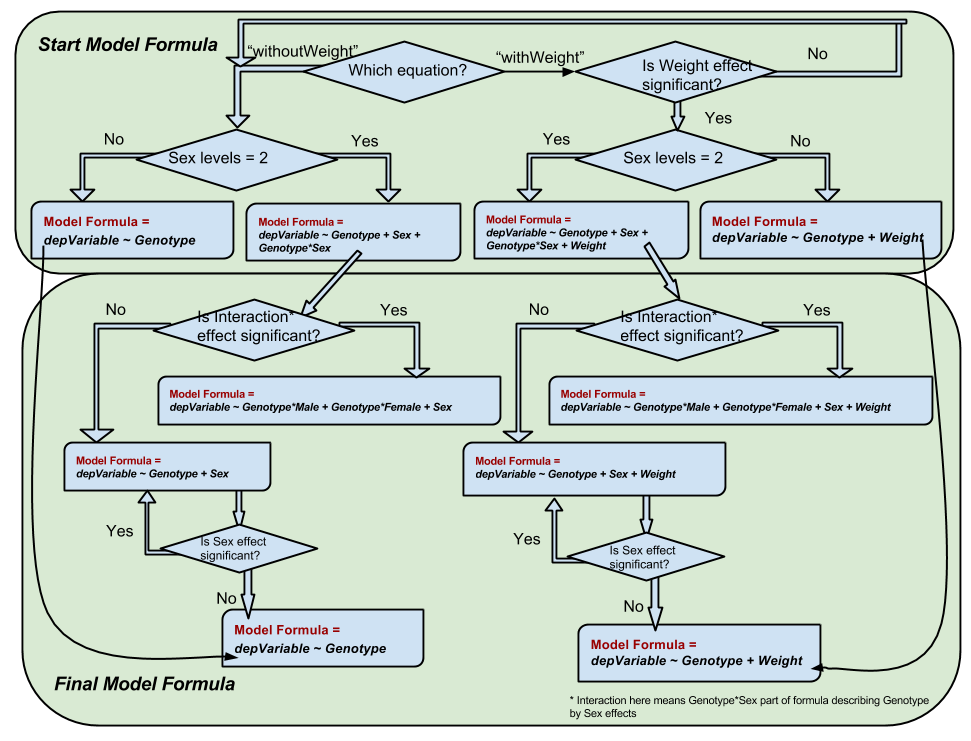
\includegraphics[scale=0.5]{Model_Formula.png}}
\caption{MM framework: start model formula and final model formula creation based on the dataset and significances of the effects (can be estimated or defined by user). }\label{fig:03}
\end{figure}

\begin{figure}[!tpb]%figure04
\centerline{\includegraphics[scale=0.5]{Mixed_Models.png}}
\caption{MM framework: different models that are considered. }\label{fig:04}
\end{figure}

When the final model is selected and reduced, the genotype effect is assessed by comparing a genotype and null model fitted with maximum likelihood evaluation method (ML). Finally, the final genotype model is refitted using restricted maximum likelihood evaluation method (REML) to get unbiased estimates of the variance parameters (see Fig. \ref{fig:02} Step 5,6 and Fig. \ref{fig:03}).   

\subsubsection{Implementation}
\label{sec:MMImplementation}
There are two functions in the PhenStat package that implements the Mixed Model framework:
\begin{itemize}
\item \textit{startModel} function evaluates model's criteria and stores the result in the \textit{PhenTestResult} object;
\item \textit{finalModel} function builds the final model using the model's criteria from \textit{PhenTestResult} object and fits the model using restricted maximum likelihood method (REML). 
\end{itemize}

By default, both functions will be called from \textit{testDataset} manager sequentially, that is why \textit{startModel} function's arguments and specific for MM method \textit{testDataset} function's arguments concur.
In the text above we mention \textit{startModel} function's arguments only. 

The equation type is defined by \textit{startModel} function's argument \textit{equation} that can take value "withWeight" which is default one and "withoutWeight". The argument defines the presence or absence of body weight effect in the model (see \ref{Eq1} and \ref{Eq2}). 
In case when there are no body weight records in the dataset \textit{startModel} sets \textit{equation} argument to "withoutWeight" automatically.

\textit{startModel} function creates start fully loaded model and modifies it after testing of different hypothesis. 
As was described in the previous theory section the model view is influenced by the number of criteria. 
Each criteria or effect (body weight effect, residual variances homogeneity, sex effect, genotype by sex interaction effect, batch effect) is evaluated individually
and TRUE/FALSE values are assigned to the appropriate sections of \textit{PhenTestResult} object based on evaluation results. 
TRUE value means that effect is significant and will be modelled. FALSE value means deletion of the effect from the model.

The package allows to assign user defined values to the effects of the model. 
If user would like to assign TRUE/FALSE values to the effects of the model that differ from calculated ones then (s)he has to define \textit{keepList} argument of \textit{startModel} functions 
which is a list of TRUE/FALSE values for each one criterion in the following order: is batch effect significant, are residual variances homogeneous, is body weight effect significant, 
is sex effect significant, is sex by genotype interaction effect significant. 
For instance, keepList=c(TRUE, TRUE, TRUE, TRUE, TRUE) defines the fully loaded model will all possible fixed effects with homogeneous residual variances; 
in turn keepList=c(FALSE, FALSE, TRUE, TRUE, TRUE) defines the fully loaded model without random effects and with heterogeneous residual variances.

\textit{startModel} function checks user defined effects for consistency (for instance, if there are no "Weight" column in the dataset then weight effect can't be assigned to TRUE, etc.)
and prints out both calculated and user defined effects (only when \textit{outputMessages} argument is set to TRUE) for the user's convenience. Note: user defined effects have a priority over calculated (evaluated) effects.

The result of the \textit{startModel} function is MM start model with reduced non-significant effects stored in the \textit{PhenTestResult} object together with the evaluated or user defined effects.
It is important to mention here the convergency problem. If for some reason, the selected model is failing to converge we simplify it by selecting the similar but simplier model and try to fit again. 
For instance, if model with heterogeneous residuals is not converging then model with homogeneous residuals will be selected.

The next step of MM framework: evaluation of genotype effect and fitting of selected model using REML is implemented in package's function \textit{finalModel}. 
The results are added into the \textit{PhenTestResult} object.  \textit{PhenTestResult} object at the end of the MM framework contains model formula, significances of the effects, genotype evaluation results and model fitting results including effect sizes.

By default both functions (\textit{startModel} and \textit{finalModel}) will be called from \textit{testDataset} manager one after another. 
We've made this logical separation of functionality in order to add more flexibility for the statisticians. 
Basically, it means that a user can check the evaluation of fixed effects and the selected model before final model fitting. 
This kind of "debugging" functionality allows the user to change some of the arguments of functions and start the model building process from scratch if needed.

We believe that the possibility to change mixed models framework behaviour as described above will help users to go deeper into details of the modelling process, 
as well as debug and compare the results from different models. 



\begingroup
    \fontsize{8pt}{12pt}\selectfont
\begin{verbatim}

# Default behaviour
> result <- testDataset(test,depVariable="Bone.Area", equation="withoutWeight")
Information:
Dependent variable: 'Bone.Area'.

Information:
Method: Mixed Model framework.

Information:
Calculated values for model effects are: keepBatch=TRUE, keepVariance=TRUE, 
keepWeight=FALSE, keepSex=TRUE, keepInteraction=FALSE.

Information:
Equation: 'withoutWeight'.

Information:
Perform all MM framework stages: startModel and finalModel

# Perform each step of the MM framework separatly
> result <- testDataset(test,depVariable="Bone.Area", equation="withoutWeight",callAll=FALSE)

Information:
Dependent variable: 'Bone.Area'.

Information:
Method: Mixed Model framework.

Information:
Calculated values for model effects are: keepBatch=TRUE, keepVariance=TRUE, 
keepWeight=FALSE, keepSex=TRUE, keepInteraction=FALSE.

Information:
Equation: 'withoutWeight'.

# Estimated model effects
> result$model.effect.batch
[1] TRUE
> result$model.effect.variance
[1] TRUE
> result$model.effect.weight
[1] FALSE
> result$model.effect.sex
[1] TRUE
> result$model.effect.interaction
[1] FALSE

> result$numberSexes
[1] 2

# Change the effect values: interaction effect will stay in the model
> result <- testDataset(test,depVariable="Bone.Area", 
equation="withoutWeight",keepList=c(TRUE,TRUE,FALSE,TRUE,TRUE),callAll=FALSE)

Information:
Dependent variable: 'Bone.Area'.

Information:
Method: Mixed Model framework.

Information:
User's values for model effects are: keepBatch=TRUE, keepVariance=TRUE, 
keepWeight=FALSE, keepSex=TRUE, keepInteraction=TRUE.

Information:
Calculated values for model effects are: keepBatch=TRUE, keepVariance=TRUE, 
keepWeight=FALSE, keepSex=TRUE, keepInteraction=FALSE.

Warning:
Calculated values differ from user defined values for model effects.

Information:
Equation: 'withoutWeight'.

> result <- finalModel(result)

> summaryOutput(result)
...
\end{verbatim}
\endgroup

\subsubsection{Diagnostics}
\label{MMDiagnostics}
There are two functions we've implemented for the automated diagnostics and classification of MM framework results: \textit{testFinalModel} and \textit{classificationTag}.
 
The first one performs diagnostic tests to assess the MM quality of fit. This includes normality tests for the two genotype levels residuals, BLUPs (best linear unbiased prediction) and 
``rotated'' residuals (\cite{RotatedResiduals04}) (last two only if applicable). There is only one argument of the function which is \textit{PhenTestResult} object. There are no arguments checks assuming that 
function is called internally from the \textit{finalModel} function. Consequently if calling directly it should be used with precaution. 

 \textit{testFinalModel} returns list of the following values:
 \begin{itemize}
  \item Reference genotype value.
  \item Normality test result (p-value) for the reference genotype's residuals.
  \item Test genotype value.
  \item Normality test result (p-value) for the test genotype's residuals.
  \item BLUPs normality test result (p-value); applicable only when there is batch random effects in the model, otherwise set to NA.
  \item ``Rotated'' residuals normality test result (p-value); applicable only when there is batch random effects in the model, otherwise set to NA.
 \end{itemize}

BLUP in statistics is best linear unbiased prediction and is used in linear mixed models for the estimation of random effects. 
See tutorial \href{http://www.extension.org/pages/61006/the-solcap-tomato-phenotypic-data:-estimating-heritability-and-blups-for-traits#.Ui4zjWRgYXc}{BLUPs} for more details.

``Rotated'' residuals are constructed by multiplying the estimated marginal residual vector by
the Cholesky decomposition of the inverse of the estimated marginal variance
matrix. The resulting ``rotated'' residuals are used to construct an empirical cumulative distribution function and pointwise standard errors. See
\href{http://biostats.bepress.com/cgi/viewcontent.cgi?article=1019&context=harvardbiostat}{Cholesky Residuals for Assessing Normal
Errors in a Linear Model with Correlated
Outcomes: Technical Report} for more details about ``rotated'' residuals.

\subsubsection{Classification Tag}
\textit{classificationTag} function returns a classification tag to assign a sexual dimorphism assessment of the phenotypic change from the results of MM framework.


\begingroup
    \fontsize{8pt}{12pt}\selectfont
\begin{verbatim}
> testFinalModel(result)
[1] "+/+"                "0.0560133469740866" "Sparc/Sparc"       
[4] "0.816672883686998"  "0.345325318416593"  "0.0480124939288989"
> classificationTag(result)
[1] "With phenotype threshold value 0.01 - both sexes equally"
\end{verbatim}
\endgroup

When the function is called through \textit{vectorOutput} function,  the tag shown in Figure \ref{fig:05} will be proceeded by the phrase “If phenotype is significant”,  meaning that globally the test has not assessed whether there was a statistical significant difference just that if there was this would be the classification if it was statistically significant.  When the function is called through \textit{summaryOutput} function or directly there is an argument \textit{phenotypeThreshold} (default value is 0.01),  which sets the significance threshold of whether there is a phenotype of interest.  If globally, the analysis indicates there is a statistically significant phenotype then the classification tag is appended to the phrase “With phenotype threshold value XXX”.

\begin{figure}[!tpb]%figure05
\centerline{\includegraphics[scale=0.6]{classificationTagMM2.png}}
\caption{Assigning a classification tag. The output of the mixed model framework is queried to assign a classification tag of how the observed phenotype was observed across the two sexes. Within the decision tree, the question “Is the effect the same for both sexes? “ is asking whether mathematically was there an interaction between the  genotype and sex. Occasionally the procedure will find that there was a significant interaction but when it comes to identifying how this occurred and quantifying the effect for each sex,  there is insufficient power.  In this scenario the classification returned states  that it “cannot classify the effect”.}\label{fig:05}
\end{figure}

The Mammalian Phenotype Ontology is under development as a community effort to provide standard terms for annotating mammalian phenotypic data and is housed and managed by the JAXS laboratory (see \href{http://www.informatics.jax.org/searches/MP_form.shtml}{MP ontology}). With the mixed model implementation, the output is very rich and a classification tag can be appended to the MP term to give richer information on the observed phenotype (e.g. abnormal circulating sodium levels – both sexes equally).  Figure \ref{fig:05_2}, details the decision tree that can be used with the MM output to interpret the results such a ontology term can be discerned and an annotation tag added when appropriate.

\begin{figure}[!tpb]%figure04
\centerline{\includegraphics[scale=0.6]{classificationTagMM_MP.png}}
\caption{Assigning a Mammalian Phenotype (MP) ontology term in the presence of sexual dimorphism. }\label{fig:05_2}
\end{figure}


\subsubsection{Model Failures and Jitter}
In this section, we would like to discuss failure of model fitting and the potential use of jitter.
At times,  the model fitting process with the MM methodology would struggle to fit a model.  In these instances,  the PhenStat method would return  an error message stating that the software can’t fit the the model  and suggest that you could try jitter or an alternate method such as reference range approach. For example,  this was seen with a Mean Corpuscular Volume dataset which had data only for male mice and the knockout mice had little variation as the majority of readings were 43 fl (shown in Fig. \ref{fig:05_x}).

\begin{figure}[!tpb]%figure05_x
\centerline{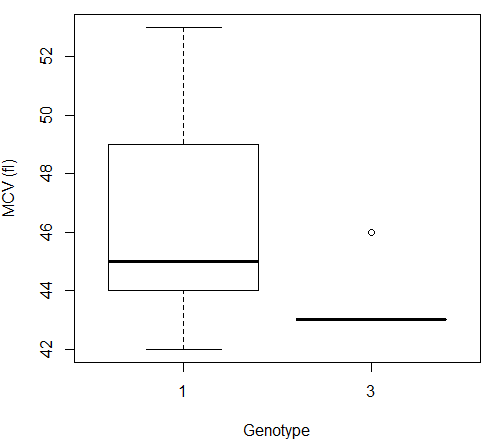
\includegraphics[scale=0.6]{Jitter_figureX.png}}
\caption{Mean corpuscular volume distribution for a dataset comparing a wildtype group (coded as 1) and a knockout group (coded as 3) of male mice.
When PhenStat processes this data,  models are not estimated as the software fails to converge on a solution and estimate the parameters,  thus the software returns the error “Error: Can’t fit the model ... Try to add jitter or RR plus method."}\label{fig:05_x}
\end{figure}

\begingroup
    \fontsize{8pt}{12pt}\selectfont
\begin{verbatim}
> file <- system.file("extdata", "test_jitter.csv", package="PhenStat") 
> dataset_jitter <- read.csv(file)

> test_jitter <- PhenList(dataset=dataset_jitter, 
   testGenotype="3", refGenotype="1",
   dataset.values.missingValue="null")
   
> result <- testDataset(test_jitter, depVariable="MCV", 
   equation="withoutWeight")
Information:
Dependent variable: 'MCV'.

Information:
Perform all MM framework stages: startModel and finalModel.

Information:
Method: Mixed Model framework.

Error:
Can't fit the model MCV ~ Genotype. Try to add jitter or RR plus method.
\end{verbatim}
\endgroup

Jitter is a function that adds a small amount of noise to a variable.  The noise is added randomly at 1000th of the signal difference for that variable.  In the example shown, the additional of noise allows the model to converge and estimate the values.
  
Code to add jitter and process the new variable:


\begingroup
    \fontsize{8pt}{12pt}\selectfont
\begin{verbatim}
> test_jitter@datasetPL$MCVWITHjitter <- jitter(test_jitter@datasetPL$MCV, 
         factor =((max(test_jitter@datasetPL$MCV) - min(test_jitter@datasetPL$MCV)) / 1000))

> result_jitter <- testDataset(test_jitter, depVariable="MCVWITHjitter",
        equation="withWeight")

Information:
Dependent variable: 'MCVWITHjitter'.
...
> summaryOutput(result_jitter)

Test for dependent variable:
*** MCVWITHjitter ***

Method:
*** Mixed Model framework ***

----------------------------------------------------------------------------
Model Output
----------------------------------------------------------------------------
Final fitted model: MCVWITHjitter ~ Genotype
Was batch significant? TRUE
Was variance equal? FALSE
Genotype p-value: 7.872660e-03
Genotype effect: 1.3082 +/- 0.4792
Was there evidence of sexual dimorphism? no (p-value NA)
Genotype percentage change Male: 2.83%

----------------------------------------------------------------------------
Classification Tag
----------------------------------------------------------------------------
With phenotype threshold value 0.01 - a significant change for the one sex tested

----------------------------------------------------------------------------
Model Output Summary
----------------------------------------------------------------------------
                Value Std.Error  DF   t-value       p-value
(Intercept) 46.293656 0.4869087 238 95.076670 2.551272e-191
Genotype3    1.308178 0.4792010 238  2.729914  6.808624e-03
\end{verbatim}
\endgroup

\subsubsection{Reporting Biological Effect}
\label{section:BiologicalEffect}
The biological effect is reported in two formats: model estimate and a percentage change. 

The first measure is on a scale specific to that variable; whilst the second is relative to the global signal and thus is scaled comparable across variables. 

The model estimate is in the scale of the variable and is the estimated change arising from being a knockout animal relative to the reference data. In the presence of sexual dimorphism the model estimate is estimated separately for the male and female knockout animals. In the \textit{summaryOutput} view these estimates are reported in the ANOVA table. In the \textit{vectorOutput} view these values are captured and reported as either Genotype estimate or Sex FvKO estimate and Sex MvKO estimate depending on whether sexual dimorphism was found to be significant.

The percentage change is the ratio of the genotype effect for a sex relative to the global average signal for that variable. The figures \ref{fig:05_be1} and \ref{fig:05_be2} show the various models and how the percentage change is estimated. The global average here is the mean value of all values from the variable of interest. The calculated percentage changes are in the \textit{summaryOutput} and reported in the \textit{vectorOutput} as "Genotype percentage change Male" and/or "Genotype percentage change Female".  

See Figures \ref{fig:05_be1} and \ref{fig:05_be2} for the percentage change calculation details.

\begin{figure}[!htpb]%figure01
\centerline{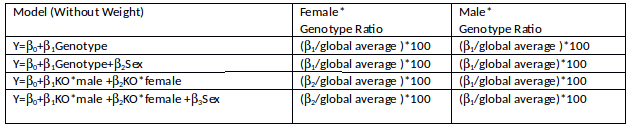
\includegraphics[scale=0.6]{BiologicalEffect4.png}}
\caption{Calculation of the percentage change for model without weight}\label{fig:05_be1}
\end{figure}

\begin{figure}[!htpb]%figure01
\centerline{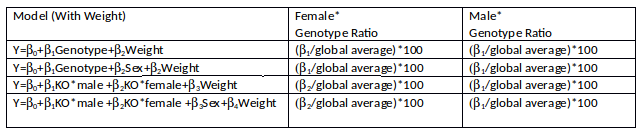
\includegraphics[scale=0.6]{BiologicalEffect3.png}}
\caption{Calculation of the percentage change for model that includes weight}\label{fig:05_be2}
\end{figure}

Example calculation:
\begingroup
\fontsize{8pt}{12pt}\selectfont
\begin{verbatim}
> file <- system.file("extdata", "test1.csv", package="PhenStat")
> test <- PhenList(dataset=read.csv(file), testGenotype="Sparc/Sparc")
...
> result <- testDataset(test,depVariable="Lean.Mass", 
			method="MM", equation="withoutWeight", transformValues=FALSE)
...			
> summaryOutput(result)
Test for dependent variable:
*** Lean.Mass ***

Method:
*** Mixed Model framework ***

----------------------------------------------------------------------------
Model Output
----------------------------------------------------------------------------
Final fitted model: Lean.Mass ~ Genotype + Sex
Was batch significant? TRUE
Was variance equal? TRUE
Genotype p-value: 6.751997e-04
Genotype effect: -1.8618 +/- 0.5418
Was there evidence of sexual dimorphism? no (p-value 6.330802e-01)
Genotype percentage change Female: -9.17%
Genotype percentage change Male: -9.17%

----------------------------------------------------------------------------
Classification Tag
----------------------------------------------------------------------------
With phenotype threshold value 0.01 - both sexes equally

----------------------------------------------------------------------------
Model Output Summary
----------------------------------------------------------------------------
                        Value Std.Error  DF    t-value       p-value
(Intercept)         18.440648 0.1696796 412 108.679253 2.044168e-305
GenotypeSparc/Sparc -1.861759 0.5417867 412  -3.436332  6.495823e-04
SexMale              4.209940 0.1607472 412  26.189818  1.018842e-89

> mean_all <- mean(test@datasetPL[,c("Lean.Mass")],na.rm=TRUE)  
[1] 20.30544

\end{verbatim}
\endgroup 
\[
Genotype\:percentage\:change\:Male = (-1.861759/20.30544)*100=-9.17\%
\]
\[
Genotype\:percentage\:change\:Female = (-1.861759/20.30544)*100=-9.17\%
\]


If the weight is included in the fitted model the results are different:
\begingroup
\fontsize{8pt}{12pt}\selectfont
\begin{verbatim}
> result <- testDataset(test,depVariable="Lean.Mass", 
				method="MM", equation="withWeight", transformValues=FALSE)
> summaryOutput(result)
Test for dependent variable:
*** Lean.Mass ***

Method:
*** Mixed Model framework ***

----------------------------------------------------------------------------
Model Output
----------------------------------------------------------------------------
Final fitted model: Lean.Mass ~ Genotype + Sex + Weight
Was batch significant? TRUE
Was variance equal? FALSE
Genotype p-value: 3.715089e-01
Genotype effect: -0.2914 +/- 0.3305
Was there evidence of sexual dimorphism? no (p-value 1.022353e-01)
Genotype percentage change Female: -1.44%
Genotype percentage change Male: -1.44%

----------------------------------------------------------------------------
Classification Tag
----------------------------------------------------------------------------
With phenotype threshold value 0.01 - no significant change

----------------------------------------------------------------------------
Model Output Summary
----------------------------------------------------------------------------
                         Value  Std.Error  DF    t-value      p-value
(Intercept)          7.6111388 0.58862654 411 12.9303357 2.512303e-32
GenotypeSparc/Sparc -0.2914357 0.33047985 411 -0.8818562 3.783700e-01
SexMale              1.6407343 0.18080930 411  9.0743913 4.791912e-18
Weight               0.3430502 0.01808121 411 18.9727422 4.147891e-58

> mean_all <- mean(test@datasetPL[,c("Lean.Mass")],na.rm=TRUE)  
[1] 20.30544
\end{verbatim}
\endgroup 
\[
Genotype\:percentage\:change\:Male = (-0.2914357/20.30544)*100 = -1.44\%
\]
\[
Genotype\:percentage\:change\:Female = (-0.2914357/20.30544)*100 = -1.44\%
\]

\subsection{Time Fixed Effect Framework}
Time Fixed Effect framework manages data variation by estimating each batch effect to separate it from genotype.
\subsubsection{Motivation}
Through high throughput phenotyping programs, such as EUMODIC, where data was systematically collected on one genetic background, the significant sources of variation can be identified and it became obvious that batch (defined here as those readings collected on a particular day) can lead to large variation in phenotyping variables \cite{MM12}. A high throughput phenotyping program will have a well-defined phenotyping pipeline which consists of a sequence of phenotyping procedures carried out at specific ages. To date, standardisation has focused on the experimental methods by which data were collected [5,6]. However the workflow -- the practical implementation of a pipeline -- varies from center to center. Each center’s workflow is a balance of resources, other goals (e.g. allowing for additional phenotyping depending on earlier results) and throughput requirements. Differences in the number and frequency of controls, whether knockout animals are phenotyped at one time or in multiple batches, and blinding methodologies are the most important variables. One strategy implemented is to accept that animals for a knockout line are obtained in small batches due to fertility or fecundity issues, but with each small batch control animals are concurrently phenotyped. This allows an analysis using a regression method where batch is treated as a fixed effect. We have called this analysis framework “Time Fixed Effect”. 
\subsubsection{Theory}
There are two possible start models, depending on whether weight is included as a factor (see \ref{Eq1TF} for the model without weight and \ref{Eq2TF} for the model including weight).

\[
depVariable \backsim Genotype + Sex +
Genotype*Sex + Batch \tag{Eq3}\label{Eq1TF}
\]
\[
depVariable \backsim Genotype + Sex +
Genotype*Sex + Weight + Batch\tag{Eq4}\label{Eq2TF}
\]

The same top-down approach can be used here as in Mixed Models framework for the model optimization process. When batch is insignificant then the Mixed Model formula is the same as Time Fixed Effect framework's formula.

As in the case of Mixed Model framework the final model construct is influenced by a number of criteria. The only one difference is that there are no random effects in the model. 

The following criteria (effects) are considered:
\begin{itemize}
\item Batch effect (batch variation). \textbf{NB!} In TF framework batch effect is a fixed effect. 
\item Residual variances homogeneity where homogeneous residual variances means the variance for all genotype levels is tested equivalent.
\item Body weight effect. Considered only when \ref{Eq2TF} is used.
\item Sex effect. Considered only when there are more than one sex in the dataset. 
\item Genotype by sex interaction effect. Considered only when there are more than one sex in the dataset. 
\end{itemize}

The selection of model is influenced by the batch effect -- is batch in the dataset, and if so, is it significant in explaining variation in the dependent variable -- and a covariance structure for the residuals that can be homogeneous or heterogeneous. The selected model is then modified by reducing non-significant effects. When the final model is selected and reduced, the genotype effect is assessed by comparing a genotype and null model fitted with maximum likelihood evaluation method (ML). Finally, the final genotype model is refitted using restricted maximum likelihood evaluation method (REML) to get unbiased estimates of the variance parameters.
\subsubsection{Implementation}
The analysis requires the removal of dates which are not concurrent with knockout animals.  This is achieved by the \textit{TFDataset} function that goes through all dataset's records and removes ones that don't have data in test genotype and in reference genotype for the same batch level (assay date) at least for one sex. Summary statistics on the cleaning impact are then provided following the table of data.  

See the example below:
\begingroup
\fontsize{8pt}{12pt}\selectfont
\begin{verbatim}
> file <- system.file("extdata", "test7_TFE.csv", package="PhenStat")
> test <- PhenList(dataset=read.csv(file),
                  testGenotype="het",
                  refGenotype = "WT",
                  dataset.colname.sex="sex",
                  dataset.colname.genotype="Genotype",
                  dataset.values.female="f",
                  dataset.values.male= "m",
                  dataset.colname.weight="body.weight",
                  dataset.colname.batch="Date_of_procedure_start")
...
> test_TF <- TFDataset(test,depVariable="Cholesterol")

Data points containing 'Cholesterol' by batch levels:
|  ----------- |  ----------- |  ----------- |  ----------- |  ----------- |
|              |           WT |           WT |          het |          het |
|  ----------- |  ----------- |  ----------- |  ----------- |  ----------- |
|        Batch |       Female |         Male |       Female |         Male |
|  ----------- |  ----------- |  ----------- |  ----------- |  ----------- |
| * 02.09.2013 |            7 |            4 |            0 |            0 |
|  ----------- |  ----------- |  ----------- |  ----------- |  ----------- |
| * 03.02.2014 |            0 |            1 |            0 |            0 |
|  ----------- |  ----------- |  ----------- |  ----------- |  ----------- |
...
|  ----------- |  ----------- |  ----------- |  ----------- |  ----------- |
| * 13.01.2014 |            4 |            2 |            0 |            0 |
|  ----------- |  ----------- |  ----------- |  ----------- |  ----------- |
| * 13.05.2013 |            7 |            5 |            0 |            0 |
|  ----------- |  ----------- |  ----------- |  ----------- |  ----------- |
| * 14.01.2014 |            5 |            7 |            0 |            0 |
|  ----------- |  ----------- |  ----------- |  ----------- |  ----------- |
|   14.04.2014 |            0 |            4 |            4 |            3 |
|  ----------- |  ----------- |  ----------- |  ----------- |  ----------- |
| * 14.10.2013 |            7 |            5 |            0 |            0 |
|  ----------- |  ----------- |  ----------- |  ----------- |  ----------- |
| * 15.07.2013 |            5 |            5 |            0 |            0 |
|  ----------- |  ----------- |  ----------- |  ----------- |  ----------- |
| * 16.06.2014 |            8 |            8 |            0 |            0 |
|  ----------- |  ----------- |  ----------- |  ----------- |  ----------- |
| * 16.09.2013 |            2 |            3 |            0 |            0 |
|  ----------- |  ----------- |  ----------- |  ----------- |  ----------- |
|   17.02.2014 |            6 |            4 |            3 |            4 |
|  ----------- |  ----------- |  ----------- |  ----------- |  ----------- |
| * 17.03.2014 |            4 |            5 |            0 |            0 |
|  ----------- |  ----------- |  ----------- |  ----------- |  ----------- |
|   18.02.2014 |            0 |            3 |            2 |            3 |
|  ----------- |  ----------- |  ----------- |  ----------- |  ----------- |
| * 18.03.2014 |            4 |            3 |            0 |            0 |
|  ----------- |  ----------- |  ----------- |  ----------- |  ----------- |
...

* - removed record(s)

Number of batch levels left: 3
Records removed (reference genotype): 92%
Records removed (test genotype): 0%
...

result <- testDataset(test_TF,depVariable="Cholesterol",method="TF")

Information:
Dependent variable: 'Cholesterol'.

Information:
Perform all TF framework stages: startTFModel and finalTFModel.

Information:
Method: Time as Fixed Effect framework.

Information:
Equation: 'withWeight'.

Information:
Calculated values for model effects are: keepBatch=TRUE, keepEqualVariance=FALSE, keepWeight=TRUE, 
keepSex=FALSE, keepInteraction=TRUE.

\end{verbatim}
\endgroup

The cleaned dataset contains only three batches which correspond to concurrent control approach. 
\begingroup
\fontsize{8pt}{12pt}\selectfont
\begin{verbatim}
|  ----------- |  ----------- |  ----------- |  ----------- |  ----------- |
|              |           WT |           WT |          het |          het |
|  ----------- |  ----------- |  ----------- |  ----------- |  ----------- |
|        Batch |       Female |         Male |       Female |         Male |
|  ----------- |  ----------- |  ----------- |  ----------- |  ----------- |
|   14.04.2014 |            0 |            4 |            4 |            3 |
|  ----------- |  ----------- |  ----------- |  ----------- |  ----------- |
|   17.02.2014 |            6 |            4 |            3 |            4 |
|  ----------- |  ----------- |  ----------- |  ----------- |  ----------- |
|   18.02.2014 |            0 |            3 |            2 |            3 |
|  ----------- |  ----------- |  ----------- |  ----------- |  ----------- |
\end{verbatim}
\endgroup

Similarly to the MM framework there are two functions in the PhenStat package that implements the Time Fixed Effect framework:
\begin{itemize}
\item \textit{startTFModel} function evaluates model's criteria and stores the result in the \textit{PhenTestResult} object;
\item \textit{finalTFModel} function builds the final model using the model's criteria from \textit{PhenTestResult} object and fits the model using restricted maximum likelihood method (REML). 
\end{itemize}
By default, both functions will be called from \textit{testDataset} manager sequentially.

\subsubsection{Diagnostics}
The vectorOutput function includes statistical tests for normality on the residuals for the wildtype and residuals for the knockout (see section \ref{MMDiagnostics}). These normality tests are provide to assist in the building automated tools for assessing model fit, however when there is a lot of data, the statistical test can be overall sensitive to departures from normality and when the number of data points is low, the test can lack ability to detect deviations from normality.

The normality tests are driven by the function \textit{testFinalModel} and it returns a list of the following values:
\begin{enumerate}
\item Reference genotype value.
\item Normality test result (p-value) for the reference genotype's residuals.
\item Test genotype value.
\item Normality test result (p-value) for the test genotype's residuals.
\item NA
\item NA
\end{enumerate}

For example:
\begingroup
\fontsize{8pt}{12pt}\selectfont
\begin{verbatim}
> testFinalModel(result)
[1] "WT"                "0.803172853943264" "het"              
[4] "0.788809875034823" NA                  NA                 
\end{verbatim}
\endgroup
Graphical methods are the recommended method for assessing model fits. Model fit quality can also be assessed graphically using \textit{qqplotGenotype},  \textit{boxplotResidualBatch} and  \textit{plotResidualPredicted} (see case study example \ref{cs_tf} for example usage).

\subsubsection{Classification Tag}
\label{TF_classificationTag}
The \textit{classificationTag} function returns a classification tag to assign a sexual dimorphism assessment of the phenotypic change from the results of the TF framework. Figure \ref{fig:05} shows the decision tree that is used to determine the tag assigned. 

\begingroup
\fontsize{8pt}{12pt}\selectfont
\begin{verbatim}
> classificationTag(result)
[1] "With phenotype threshold value 0.01 - both sexes equally"
\end{verbatim}
\endgroup

When the function is called through \textit{vectorOutput} function, the tag will be proceeded by the phrase “If phenotype is significant", meaning that globally the test has not assessed whether there was a statistical significant difference just that if there was this would be the classification if it was statistically significant. When the function is called through \textit{summaryOutput} function or directly there is an argument \textit{phenotypeThreshold} (default value is 0.01), which sets the significance threshold of whether there is a phenotype of interest. If globally, the analysis indicates there is a statistically significant phenotype then the classification tag is appended to the phrase “With phenotype threshold value XXX".

\subsubsection{Reporting Biological Effect}
Within Time Fixed Effect framework the biological effect is also reported in two formats: model estimate and a percentage change. The meaning of the calculated values is the same as in Mixed Model framework. Please see section \ref{section:BiologicalEffect} for details. 
\subsection{Fisher Exact Test Framework}
\label{section:FET}
Fisher Exact Test is a standard framework for categorical data which compares data proportions and calculates the percentage change in classification. 
\subsubsection{Motivation}
A Fisher Exact Test was chosen as most abnormal phenotype traits are rare event thus the signal is low. Batch is not considered significant because day to day variation does not effect abnormality call for these types of variables.
\subsubsection{Implementation}
The Fisher Exact Test is implemented with basic R functions from the stats package after the construction of count matrices (also called chi squared tables) from the dataset. 

Together with count matrices we also calculate percentage matrices for effect size calculation.

From the chi squared table statistical significance is assessed using a Fisher Exact Test whilst the biological significance is estimated by an effect size (see section \ref{FE_EffectSize} for more details).

These are calculated separately for 3 subsets (if there are multiple sex values in the dataset):
\begin{itemize}
 \item combined dataset (regardless the sex values),
 \item males only subset,
 \item females only subset.
\end{itemize}

All results are stored in \textit{PhenTestResult} object:

\begingroup
\fontsize{8pt}{12pt}\selectfont
\begin{verbatim}
> file <- system.file("extdata", "test_categorical.csv", package="PhenStat") 
> dataset_cat <- read.csv(file)

> test_cat <- PhenList(dataset=dataset_cat, testGenotype="Aff3/Aff3")
 
Warning:
Dataset's column 'Assay.Date' has been renamed to 'Batch' and will be used for the batch effect modeling.

Warning:
Dataset has been cleaned by filtering out records with genotype value 
other than test genotype 'Aff3/Aff3' or reference genotype '+/+'.

Warning:
Dataset's 'Weight' column is missed.
You can define 'dataset.colname.weight' argument to specify column 
for the weight effect modeling. Otherwise you can only use mixed model equation 'withoutWeight'.

Information:
Dataset's 'Genotype' column has following values: '+/+', 'Aff3/Aff3'

Information:
Dataset's 'Sex' column has following value(s): 'Female', 'Male'

> result_cat <- testDataset(test_cat,
 depVariable="Thoracic.Processes",
 method="FE")

Information:
Dependent variable: 'Thoracic.Processes'.

Information:
Method: Fisher Exact Test framework.

> result_cat@depVariable
[1] "Thoracic.Processes"
> getVariable(result_cat)
[1] "Thoracic.Processes"
> result_cat@method
[1] "FE"
> method(result_cat)
[1] "FE"
> noSexes(result_cat)
[1] 2

# Chi squared table for all data
> getCountMatrices(result_cat)$all
         +/+ Aff3/Aff3
Abnormal 142        12
Normal   753         1

# Chi squared table for males only records
> getCountMatrices(result_cat)$male
         +/+ Aff3/Aff3
Abnormal  59         5
Normal   390         1

# Percentage matrix for all data
> result_cat$model.output$percentage_matrix_all

         +/+ Aff3/Aff3 ES change
Abnormal  16        92        76
Normal    84         8        76

# Percentage matrix for females only records
> getPercentageMatrix(analysisResults(result_cat)[[3]])

              +/+ Aff3/Aff3
Abnormal 15.86592 92.307692
Normal   84.13408  7.692308

# Effect size for all data
> analysisResults(result_cat)[[1]]@ES
[1] 76

# Effect size for females only records
> analysisResults(result_cat)[[3]]@ES
[1] 81

# Fisher Exact Test results for all data
> analysisResults(result_cat)[[1]]@modelOutput

	Fisher's Exact Test for Count Data

data:  count_matrix_all 
p-value = 4.844e-09
alternative hypothesis: true odds ratio is not equal to 1 
95 percent confidence interval:
 0.0003770171 0.1096287774 
sample estimates:
odds ratio 
 0.0159923
 
# p-value for all data
> pvalue(analysisResults(result_cat)[[1]])
[1] 4.844291e-09
\end{verbatim}
\endgroup

The same data as shown in examples can be obtained by using output functions of the package: \textit{summaryOutput}, \textit{vectorOutput} and \textit{vectorOutputMatrices}. See section \ref{section:Results} for more details.

If there is only one level for the dependent variable in the dataset e.g. "Normal`` then the package will add level "Other'' into the count matrices for consistency. All values for this level will be set to 0.
The following is an example of such case:


\begingroup
    \fontsize{8pt}{12pt}\selectfont
\begin{verbatim}
> file <- system.file("extdata", "test_categorical_normal.csv", package="PhenStat") 
> dataset_cat_normal <- read.csv(file)
> test2 <- PhenList(dataset=dataset_cat_normal, testGenotype="Aff3/Aff3")
> result2 <- testDataset(test2,depVariable="Thoracic.Processes", method="FE")
> levels(factor(result2@analysedDataset$Thoracic.Processes))
[1] "Normal"
> summaryOutput(result2)

Test for dependent variable:
*** Thoracic.Processes ***

Method:
*** Fisher Exact Test framework ***

----------------------------------------------------------------------------
Model Output ('*' highlights results with p-values less than threshold 0.01)
----------------------------------------------------------------------------
All                
  p-value:     1.0000
  Effect size: 0%    

Males only         
  p-value:     1.0000
  Effect size: 0%    

Females only    
  p-value:     1.0000
  Effect size: 0%    

----------------------------------------------------------------------------
Classification Tag
----------------------------------------------------------------------------
Not significant

----------------------------------------------------------------------------
Count Matrices
----------------------------------------------------------------------------
All
       +/+ Aff3/Aff3
Normal 895        13
Other    0         0

Males only
       +/+ Aff3/Aff3
Normal 449         6
Other    0         0

Females only
       +/+ Aff3/Aff3
Normal 446         7
Other    0         0
\end{verbatim}
\endgroup
\subsubsection{Classification Tag}
We've implemented the function \textit{classificationTag} also for the FE framework. 
However, in the case of Fisher Exact Test it is not sexual dimorphism classification, but rather the overall estimation of the signals significance across the different datasets.

Having the Fisher Exact Test results for three datasets: males only, females only, all (combined set) the p-values are compared with \textit{phenotypeThreshold} argument which default value is 0.01. For each one set the function calculates is genotype significant or not (significant if p-value is less than \textit{phenotypeThreshold}) and then assigns classification tag. In the Table \ref{table:06}, the possible classification tags are presented.  

\begin{table}[H]
\begin{center}
\begin{tabular}{| p{8mm} | p{13mm} | p{10mm} | p{13mm} | p{15mm} | p{7cm} |}
  \hline
No sexes& \multicolumn{4}{c}{Genotype significant in }&Classification Tag\\
&general&males only&females only&combined set&\\

\hline
1&yes&-&-&yes&Significant for the sex tested\\
1&no&-&-&no&Not significant\\
2&no&no&no&no&Not significant\\
2&yes&no&no&yes&Significant in males and in combined dataset\\
2&yes&no&yes&no&Significant in females dataset only\\
2&yes&yes&no&no&Significant in males dataset only\\
2&yes&yes&no&yes&Significant in males and in combined dataset\\
2&yes&yes&yes&no&Significant in males and in females dataset\\
2&yes&no&yes&yes&Significant in females and in combined dataset\\
2&yes&yes&yes&yes&Significant in males, females and in combined dataset\\
\hline  
\end{tabular}
\caption{Classification tag assignment by using Fisher Exact Tests results for three sets: males only, females only, all (combined set).}\label{table:06}
\end{center}
\end{table}

\subsection{Reference Range Plus Framework}
At times phenotyping data has been collected in such a way, that typical analysis routes are not considered reliable. The conservative, easy to understand reference range method (RR framework) can have a role in identifying phenodeviants.   
\subsubsection{Theory}
The reference range methodology is considered a conservative method where data are classed normal, low or high depending on whether they lie within the natural variation seen within the control. 

\begin{figure}[H]%figure01a
\centerline{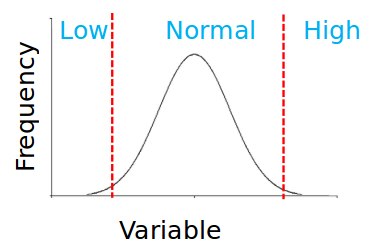
\includegraphics[scale=0.4]{RR1_simple.png}}
\caption{Control data are used to find the ranges for normal, low and high classifications.}
\end{figure} 

Once the data are classified by using the ranges calculated from control data, then a Fisher Exact Test is used to compare the movement towards the low or high classification. 

\begin{figure}[H]%figure01a
\centerline{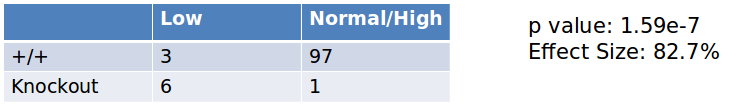
\includegraphics[scale=0.4]{RR2_1_simple.png}}
\centerline{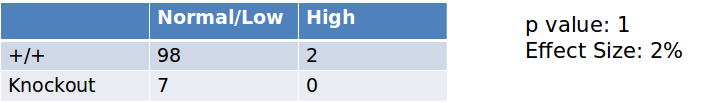
\includegraphics[scale=0.4]{RR2_2_simple.png}}
\caption{Fisher Exact Test is used to calculate p-values.}
\end{figure} 

\subsubsection{Implementation}
The RR methodology is driven from the \textit{testDataset} function manager. To analyse the data using the RR methodology the argument \textit{method} needs to be set to "RR".  For the RR methodology there are a number of additional arguments that determine how the RR is executed. The \textit{RR\_naturalVariation} argument (defaults to 95, minimal value is set to 60) determines how much of the data is classified as normal and thus is used in the calculations of the classification threshold. The thresholds are determined using a percentile method, which avoids any distribution assumptions. 
For example, when \textit{RR\_naturalVariation} defaults to 95, then 95\%  of the data will be classed as normal, i.e. the 2.5 and 97.5 percentile thresholds of the dependent variable are used to define the boundaries of normal. 

The \textit{RR\_controlPointsThreshold} argument (defaults to 60)  determines the minimum number of data points per sex that are used to determine a reference range.  Since the mathematical minimum is recommended as 40 data points (see \cite{Solberg} for details) \textit{RR\_controlPointsThreshold} minimal value is also set to 40.

Data is analysed in three ways: 1) male only, 2) female only, and 3)  all (combined dataset). In the all classification, the classifications of normal, low, and high are combined in the count table but please note the classification to normal, low, or high are run on a sex specific basis.  In the situation where only one sex is present the output is returned in the all category.

If we had compared normal vs low and high classification simultaneously there would have been a potential problem of having a highly significant p-value yet an ES that is low. This can arise when there is movement away from the normal classification to both a low and high classification at the same time. As people want to use one filter this was a problem. 

Our solution is to compare movement towards low separately from movement towards high classifications. As a result an adjustment for the multiple testing is needed (we use simple multiplication of p-value by two) since there are two tests performed: low vs normal/high (low classification) and high vs normal/low (high classification).  

The effect size calculated is the maximum percentage change seen in the low and high classification. For each trait level (i.e. the observed phenotype), the change in percentage effect size is seen by subtracting the percentage observed in the knockout from the control.

All results are stored in \textit{PhenTestResult} object:

\begingroup
\fontsize{8pt}{12pt}\selectfont
\begin{verbatim}
> file <- system.file("extdata", "test_Akt2.csv", package="PhenStat") 
> DEXAdata <- read.csv(file)
> test <- PhenList(dataset=DEXAdata,
		  testGenotype="Akt2/Akt2",
		  refGenotype="WT",
		  dataset.colname.batch="dateOfExperiment",
		  dataset.values.female="female",
		  dataset.values.male="male", 
		  dataset.colname.genotype="Genotype", 
		  dataset.colname.sex="Gender")
...		  
> result <- testDataset(test, 
			depVariable="Lean.Mass", 
			method="RR")
...			
> summaryOutput(result)

Test for dependent variable:
*** Lean.Mass ***

Method:
*** Reference Ranges Plus framework ***

1) High vs Normal/Low
           All Females only Males only
p-value 1.0000       1.0000     1.0000
ES          3%           3%         3%

2) Low vs Normal/High
           All Females only Males only
p-value 0.0000       0.0000     0.0000
ES         59%          72%        47%

----------------------------------------------------------------------------
Classification Tag
----------------------------------------------------------------------------
With phenotype threshold value 0.01 - significant in males (Low), females (Low) and in combined dataset (Low)

----------------------------------------------------------------------------
Thresholds
----------------------------------------------------------------------------
Natural variation:            95                  
Min control points:           60                  
Normal values 'males only':   18.10925 to 30.0315 
Normal values 'females only': 14.38975 to 23.52675

----------------------------------------------------------------------------
Count Matrices
----------------------------------------------------------------------------
All
              WT Akt2/Akt2
Low           30        16
Normal/High 1116        10

All
             WT Akt2/Akt2
High         30         0
Normal/Low 1116        26

Females only
             WT Akt2/Akt2
Low          15         9
Normal/High 559         3

Males only
             WT Akt2/Akt2
Low          15         7
Normal/High 557         7

Females only
            WT Akt2/Akt2
High        15         0
Normal/Low 559        12

Males only
            WT Akt2/Akt2
High        15         0
Normal/Low 557        14
\end{verbatim}
\endgroup 

\subsubsection{Classification Tag}
We've also implemented the function \textit{classificationTag}  for the RR framework with the same restrictions as for Fisher Exact Test -- it is not sexual dimorphism classification, but rather the overall estimation of the signals significance across various datasets.

The table of possible classification tags is very similar to the Fisher Exact Test classification table (see Table \ref{table:06}) with one additional element: next to each one dataset name (males only, females only, combined) we added the classification movement value. The possible values are "Low, "High" and "NA". "NA" value is assigned when there are both low and high classifications significant for the particular subset.

For example, if in all three subsets the genotype is significant and movement is classified as "high" the classification tag is "Significant in males (High), females (High) and in combined dataset (High)".

\subsection{Logistic Regression Framework}
Logistic Regression Framework is a framework suitable for categorical data when the variable of interest has been recoded to 0 and 1. This method models the relationship between the variable of interest and a number of independent variables assessing the impact of sex, genotype and whether the genotype effect depends on the sex.   

\subsubsection{Motivation}
The logistic regression allows the assessment of the genotype impact on phenotype for both sexes simultaneously and allows a statistical assessment of whether the genotype effect has a sexual dimorphic element. The inclusion of both sexes simultaneously increases statistical power and by the inclusion of a sexual dimorphic assessment allows a more refined assessment of the genotype effect.  

The approach implemented uses the "logistf" package of R, which is a biased reduction logistic regression which provides a refinement to the logistic regression method to allow studies with rare event categorical data \cite{Heinze}.   

The "logistf" package does not support the inclusion of random effects which was used in the MM framework to model batch in high throughput studies. This is not an issue for the majority of genotype-phenotype studies on categorical data as the phenotype traits are typically rare events studies looking for rare abnormal phenotypes and day to day variation would not influence this phenotype. 

\subsubsection{Theory}
The method starts with equation X

depVariable =  Genotype + Sex + Genotype * Sex 	(EqLR)
\[
depVariable \backsim Genotype + Sex +
Genotype*Sex \tag{Eq5}\label{EqLR}
\]

The same top-down approach is used here as in Mixed Models framework for the model optimization process, though the model optimisation steps are fewer compared to the mixed model method.  The optimisation considers two aspects assessing whether they statistically significant (p-value less than 0.05) in explaining variation in the model before selecting the final model: 

\begin{itemize}
\item Sex effect. Considered only when there are more than one sex in the dataset.
\item Genotype by sex interaction effect. Considered only when there are more than one sex in the dataset.
\end{itemize}
As an exploration validation test, we have built a routine in to assess whether batch was significant however it cannot influence the final fitted model as the biased reduction methodology used here cannot work with random effects.

When the final model is selected and reduced, the genotype effect is assessed by comparing a genotype and null models. Finally, the final genotype model is fitted to estimate the effects associated with each term included in the model.

Unlike standard regression which returns estimates (coefficients) that predict the change in the dependent variable for one unit change in the independent variable, Logistic Regression is looking at probabilities. The Logistic Regression model estimates are still measures of the contribution to variations in the dependent variable but as a log odd estimate. To increase interpretability you can relate this back to the experiment by converting the estimate into an odds ratio by calculating the exponential of the value (i.e. E\textsuperscript{$\beta$} or exp(\textsuperscript{$\beta$})). Where an odds ratio is an indicator of the change in odds resulting from a unit change in the predictor. For example, with an odds ratio of 2 which tells us that being a testGenotype animal leads to a 7.4 higher odds of being abnormal.

\subsubsection{Implementation}
The analysis requires the recoding of the data to 0 and 1 where 0 is the reference phenotype and 1 is the abnormality. This is achieved by the \textit{LRDataset} function that recodes all abnormal phenotypes as 1 and the remainder as 0. 

Similarly to the MM framework there are two functions in the PhenStat package that implements the Logistic Regression Effect framework:
\begin{itemize}
\item \textit{startLFModel} function evaluates model's criteria and stores the result in the PhenTestResult object;
\item \textit{finalLFModel} function builds the final model using the model's criteria from PhenTestResult object and assesses the genotype effect and fits the final model.
\end{itemize}
By default, both functions will be called from \textit{testDataset} manager sequentially.

See the example below:
\begingroup
\fontsize{8pt}{12pt}\selectfont
\begin{verbatim}
> file <- system.file("extdata", "test_categorical.csv", package="PhenStat")
> test <- PhenList(dataset=read.csv(file),
                  testGenotype="Aff3/Aff3")
> test2 <- LRDataset(test, depVariable="Thoracic.Processes",
				  abnormalValues="Abnormal")
> result2 <-testDataset(test2,depVariable="Thoracic.Processes",method="LR")
> summaryOutput(result2)

Test for dependent variable:
*** Thoracic.Processes ***

Method:
*** Logistic Regression ***

----------------------------------------------------------------------------
Model Output
----------------------------------------------------------------------------
Final fitted model: Thoracic.Processes ~ Genotype + Sex
Was batch significant? FALSE
Genotype p-value: 1.943939e-09
Genotype effect: 3.7983 +/- 0.9034
Was there evidence of sexual dimorphism? no (p-value 5.441219e-01)

----------------------------------------------------------------------------
Classification Tag
----------------------------------------------------------------------------
With phenotype threshold value 0.01 - both sexes equally

----------------------------------------------------------------------------
Model Output Summary
----------------------------------------------------------------------------
                       Value Std.Error   ci.lower    ci.upper      p-value
(Intercept)       -1.4646494 0.1209814 -1.7077333 -1.23321580 0.000000e+00
GenotypeAff3/Aff3  3.7983232 0.9033813  2.3619588  6.02332990 1.943939e-09
SexMale           -0.4251768 0.1840563 -0.7891747 -0.06661705 2.002838e-02
\end{verbatim}
\endgroup

\subsubsection{Classification Tag}
The \textit{classificationTag} function returns a classification tag to assign a sexual dimorphism assessment of the phenotypic change from the results of the LR framework. Figure \ref{fig:05} shows the decision tree that is used to determine the tag assigned.

\begingroup
    \fontsize{8pt}{12pt}\selectfont
\begin{verbatim}
> classificationTag(result)
[1] "With phenotype threshold value 0.01 - both sexes equally"
\end{verbatim}
\endgroup

When the function is called through \textit{vectorOutput} function, the tag will be proceeded by the phrase “If phenotype is significant", meaning that globally the test has not assessed whether there was a statistical significant difference just that if there was this would be the classification if it was statistically significant. When the function is called through \textit{summaryOutput} function or directly there is an argument phenotypeThreshold (default value is 0.01), which sets the significance threshold of whether there is a phenotype of interest. If globally, the analysis indicates there is a statistically significant phenotype then the classification tag is appended to the phrase “With phenotype threshold value XXX".

\subsubsection{Understanding the estimates}
The model estimates represent change in the probability of being a member of the modeled categories (e.g. female versus male or refGenotype versus testGenotype).  The estimated coefficients are expressed in log units and are not directly interpretable. They can be converted to an odds ratio by taking the coefficient and using it as the power to which the base of the natural logarithm (2.71828) is raised, the result represents the change in the odds of the modeled event associated with a one-unit change in the independent variable (i.e. for sex going from female to male or for genotype going from refGenotype to the testGenotype). 
If a coefficient is positive, its transformed log value will be greater than one, meaning that the modeled event is more likely to occur. If a coefficient is negative, its transformed log value will be less than one, and the odds of the event occurring decrease. A coefficient of zero (0) has a transformed log value of 1.0, meaning that this coefficient does not change the odds of the event one way or the other.

\section{Data Transformation}
\label{section:transformation}
The \textit{testDataset} function has an argument “transformValues" which can be set to TRUE or FALSE. By default the value is set to FALSE meaning NOT to perform transformation.

The "MM" and "TF" regression methods make an assumption of normally distributed data. Unfortunately at times, a non-linear transformation is needed to improve the distribution of the data to improve the model fitting reliability. 
The Box-Cox transformation (\cite{BoxCox}) represents a family of power transformations with a procedure to find the normalizing transformation for each variable. The procedure returns the optimal lambda value that specifies the transformation necessary and the procedure identifies the value by testing a variety of lambda values. The Box-Cox power transformation is not a guarantee for normality as the procedure looks to minimise standard deviation based on the assumption that the transformed data has the highest likelihood to be normally distributed when the standard deviation is the smallest. 
The Box-Cox transformation of the variable is defined as:

\begin{equation}
  y_i'=\begin{cases}
    \frac{(y_i + scaleShift)^\lambda - 1}{\lambda}, & \text{if $\lambda \neq 0$}\\
    \ln(y_i + scaleShift), & \text{otherwise}
  \end{cases}
\end{equation}

The parameter $\lambda$ is estimated using the profile-likelihood function. The parameter \textit{scaleShift} is a scaling correction for negative data.
The Box-Box transformation incorporates many tradition transformations (table \ref{table:tr1}). 
\begin{table}[!h]
\begin{center}
\begin{tabular}{| l | l | c | c |}
  \hline
$\lambda$&\multicolumn{2}{|c|}{Transformation equivalent}\\\hline
&Name&Specification\\\hline
0.5&Square root transformation&$\sqrt{Y}$\\
0.33&Cube root transformation&$\sqrt[3]{Y}$\\
0.25&Fourth root transformation&$\sqrt[4]{Y}$\\
0&Log transformation&$\ln(Y)$\\
-0.5&Reciprocal square root transformation&$\frac{1}{\sqrt{Y}}$\\
-1&Reciprocal transformation&$\frac{1}{Y}$\\
-2&Reciprocal power 2 transformation&$\frac{1}{Y^2}$\\
\hline  
\end{tabular}
\caption{Relationship between lambda and common transformations.}\label{table:tr1}
\end{center}
\end{table}

PhenStat has an implementation of the Box-Cox transformation to determine if a transformation is needed and if so how the data should be transformed. 
Implementation steps:
\begin{enumerate}
\item  \textbf{Scaling assessment}

The Box-Cox power transformation only works if all the data is positive and greater than 0. This can be achieved by adding a scaling correction (\textit{scaleShift}) to all data before it is transformed. This value if required is returned in both the \textit{summaryOutput} and the \textit{vectorOutput} functions. 
\item \textbf{Determine Lambda}

The Box-Cox procedure is applied to the data taking into account structure in the data by specifying them as fixed effects and use profile-likelihood techniques to derive the optimal $\lambda$ and the 95\% confidence interval for $\lambda$.
\item  \textbf{Convert output to transformation requirement}
\begin{itemize}
\item If the statistical method is "FE", "LR" or "RR" or if the user has chosen to perform analysis without data transformation (\textit{testDataset} function's argument \textit{transformValues} is set to FALSE) then no transformation is needed ("lambda=NA, scaleShift=NA, transformed=FALSE, code=0")
\item If the 95\% confidence interval for $\lambda$ includes 1 then no transformation is needed ("lambda=value, scaleShift=value, transformed=FALSE, code=1").
\item If the $\lambda$ value is between -0.1 and 0.1, at the same time 1 is not included into the 95\% confidence interval for $\lambda$ then the value is classed as 0 and a log transformation is performed ("lambda=0, scaleShift=value, transformed=TRUE, code=2"). 
\item If the optimal $\lambda$ value exceeds 5 or -5 then we consider that transformation is not appropriate ("lambda=value, scaleShift=value, transformed=FALSE, code=4"). 
This has been implemented as with these large $\lambda$ values the resulting transformed variable would have values that were too large/small for meaningful regression analysis. This can happen with small datasets or datasets that are poorly suited to regression analysis (e.g. datasets with little variation). 
\item For all other lambda values the implementation performs power transformation using  the optimal $\lambda$ value ("lambda=value, scaleShift=value, transformed=TRUE, code=3").  
\end{itemize}
\end{enumerate}

\textit{VectorOutput} results concerning transformation are classified in table \ref{table:tr2}.
\begin{table}[!h]
\begin{center}
\begin{tabular}{| c | c | c | p{8cm} |}
\hline
Code&$\lambda$&Values transformed&Comment\\\hline
0&NA&No&Statistical method doesn't required data transformation or user requested to perform without transformation.\\
1&value&No&According to test results transformation is not needed.\\
2&0&Yes&Log transformation is applied.\\
3&value&Yes&Power transformation is applied.\\
4&value&No&Optimal lambda value is not found within a range of -5 to 5.\\
\hline
\end{tabular}
\caption{VectorOutput values explaining transformation.}\label{table:tr2}
\end{center}
\end{table}

As shown in figure \ref{fig:tr1}, the transformation recommended by PhenStat package lead to an improvement in the residual distribution improving the model fit.  

\begin{figure}[!htpb]%figure01
\centerline{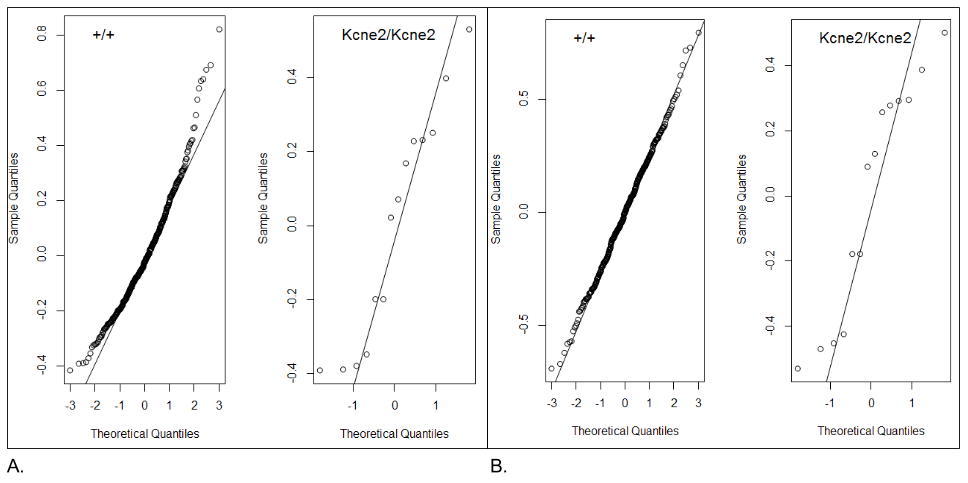
\includegraphics[scale=0.5]{transformation_example.png}}
\caption{Impact of transformation on model residuals. Mixed model analysis of the \textit{Kcne2} knockout of blood plasma triglyceride data obtained at the Wellcome Trust Sanger Institute. PhenStat transformation assessment recommended a log transformation. \textbf{A:}  Residuals obtained on fitting a model to the raw data.  \textbf{B:}  Residuals obtained on fitting a model to the PhenStat transformed data. }\label{fig:tr1}
\end{figure}

After transformation the model estimates are on a new scale and hence for interpretability it can be useful to convert these values back to the original scale.  In the \textit{summaryOutput} function, the genotype estimate and standard error is converted and this is reported as “Genotype effect (original scale)”. 
For a database users, or if you are interested in other model variables, below are the conversion functions:

\begin{equation}
  y_i=\begin{cases}
    sign(y_i' * \lambda+1) * |y_i' * \lambda+1| ^\frac{1}{\lambda} - scaleShift, & \text{if $\lambda \neq 0$}\\
    e^{y_i'} - scaleShift, & \text{otherwise}
  \end{cases}
\end{equation}
\[
    sign(x)=\begin{cases}
    1, & \text{if $x > 0$}\\
    0, & \text{if $x = 0$}\\
    -1, & \text{if $x < 0$} 
  \end{cases}
\]

\section{PhenTestResult Object}
The output of the \textit{testDataset} function is the \textit{PhenTestResult} object regardless the statistical method used. The following data are stored in this object:
\begin{itemize}
\item a subset that actually was analysed (slot \textit{analysedDataset}) with the following columns: original values of dependent variable, sex values and genotype values, transformed values of dependent variable if transformation was applied, batch values and batch adjusted values of dependent variable if batches are present in the dataset, weight values if weight is in the dataset;
\item a name of the variable that was analysed (slot \textit{depVariable});
\item reference and test genotypes (slots \textit{refGenotype} and \textit{testGenotype}), 
\item information about transformation if it was applied (slots \textit{transformationRequired}, \textit{lambdaValue} and \textit{scaleShift});
\item statistical method used and method's parameters (slots \textit{method} and \textit{parameters});
\item analysis results (slot \textit{analysisResults}).
\end{itemize} 

There is a number of useful methods available for the \textit{PhenTestResult} object, like \textit{batchIn} and \textit{weightIn} to figure out the batch/weight presence, \textit{noSexes} to get a number of sex values available in the dataset, etc.


If transformation of original data has been performed it is useful to plot the dataset based graphics to see the transformation effect. In such a case method called \textit{analysedDatasetPhenList} will output the PhenList object with transformed values. This object is used as an input argument for the graphic functions.

There is also a method specific for regression analysis methods (MM, TF, LR): \textit{getGenotypeEffect} to get report of biological effect and a method specific for the Fisher Exact Test based frameworks (FE, RR): \textit{getCountMatrices} to obtain all count matrices.

The content of the \textit{analysisResults} slot depends on the statistical method that has been used. It contains output of regression analysis for MM, TF and LR frameworks and number of "htest" objects with additional meta data (like subset, classification, effect size, count matrix) for  
Fisher Exact Test based frameworks (FE, RR). "htest" class  is used by \textit{fisher.test} function to return Fisher Exact Test results.

"FE" framework returns \textit{analysisResults} slot with  a list of 3 (1 in case of one sex only) extended "htest" objects since there are three subsets: "all", "males only", "females only".
"RR" framework returns \textit{analysisResults} slot that contains a list of 6 (2 in case of one sex only) extended "htest" object since there are three subsets ("all", "males only", "females only") and two classifications (low and high).

There are special methods available for the extended "htest" objects. For example: \textit{matrixCount} to get count matrix, \textit{getPercentageMatrix} to obtain percentage matrix, \textit{getColumnView} to obtain p-value and ES value together with meta data.

\begingroup
    \fontsize{8pt}{12pt}\selectfont
\begin{verbatim}
> file <- system.file("extdata", "test_Akt2.csv", package="PhenStat") 
> DEXAdata <- read.csv(file)
> test <- PhenList(dataset=DEXAdata,
		  testGenotype="Akt2/Akt2",
		  refGenotype="WT",
		  dataset.colname.batch="dateOfExperiment",
		  dataset.values.female="female",
		  dataset.values.male="male", 
		  dataset.colname.genotype="Genotype", 
		  dataset.colname.sex="Gender")
> result <- testDataset(test, 
			depVariable="Lean.Mass", 
			method="RR")
			
# print out count matrices and percentage matrices for male only subset			
> for (i in seq_along(analysisResults(result))) {
     val <- analysisResults(result)[[i]]
     if (analysedSubset(val)=="males"){
     	 print(comparison(val))
     	 print("Count matrix")
         print(matrixCount(val))   
         print("Percentage matrix")
         print(getPercentageMatrix(val))     
     }
 }
[1] "Low vs Normal/High"
[1] "Count matrix"
             WT Akt2/Akt2
Low          15         7
Normal/High 557         7
[1] "Percentage matrix"
                   WT Akt2/Akt2
Low          2.622378        50
Normal/High 97.377622        50
[1] "High vs Normal/Low"
[1] "Count matrix"
            WT Akt2/Akt2
High        15         0
Normal/Low 557        14
[1] "Percentage matrix"
                  WT Akt2/Akt2
High        2.622378         0
Normal/Low 97.377622       100
\end{verbatim}
\endgroup 
\section{Method Recommendation for Dataset}
\label{section:Recommendation}

Sometimes the analysis path to follow is obvious. For example, the variable "head shape" with options "Normal" or "Abnormal" is clearly categorical and therefore the Fisher Exact Test (FE) framework appropriate. At times, it is however less obvious. An example, could be the variable "number of vertebrates". Initial as this is a number this suggest continuous methods (e.g. MM, TF or RR)  however on inspection there is no variation and in fact this variable is best treated as categorical. Based on our experience, we have prepared a function called \textit{recommendMethod} which explores the data and makes recommendations on analysis that can be conducted. Please note, at times multiple analysis paths could be suitable. 


\begingroup
\fontsize{8pt}{12pt}\selectfont
\begin{verbatim}
file <- system.file("extdata", "test1.csv", package="PhenStat")

test <- PhenList(dataset=read.csv(file),
            testGenotype="Sparc/Sparc")
...

recommendMethod(test,"Lean.Mass")
...

[1] "MM and RR"
\end{verbatim}
\endgroup

Function \textit{recommendMethod} goes through all common and framework's specific checks and makes recommendations according to the check failure/success results.  
\section{Output of Results}
\label{section:Results}
The PhenStat package stores the results of statistical analyses in the \textit{PhenTestResult} object.  
For numeric summary of the analysis, there are two functions to present \textit{PhenTestResult} object data to the user: 
\textit{summaryOutput} that provides a printed summary output and \textit{vectorOutput} that creates a vector form output. 
These output forms were generated for differing users needs. 

\subsection{Summary Output}
\label{SummaryOutput}
The \textit{summaryOutput} function supports interactive analysis of the data and prints results on the screen.

The following is an example of summary output of MM framework:
\begingroup
\fontsize{8pt}{12pt}\selectfont
\begin{verbatim}
 # Mixed Model framework
> file <- system.file("extdata", "test1.csv", package="PhenStat") 

> dataset1 <- read.csv(file)

> test <- PhenList(dataset=dataset1,
    testGenotype="Sparc/Sparc",outputMessages=FALSE)
    
> result <- testDataset(test,
    depVariable="Lean.Mass",outputMessages=FALSE, transformValues=FALSE)

> summaryOutput(result)

Test for dependent variable:
*** Lean.Mass, power transformed with lambda value = -0.7  ***

Method:
*** Mixed Model framework ***

----------------------------------------------------------------------------
Model Output
----------------------------------------------------------------------------
Final fitted model: Lean.Mass ~ Genotype + Sex + Weight
Was batch significant? TRUE
Was variance equal? TRUE
Genotype p-value: 1.141215e-01
Genotype effect (original scale): 0.9962 +/- 1.0025
Was there evidence of sexual dimorphism? no (p-value 8.917040e-01)
Genotype percentage change Female: -0.31%
Genotype percentage change Male: -0.3%

----------------------------------------------------------------------------
Classification Tag
----------------------------------------------------------------------------
With phenotype threshold value 0.01 - no significant change

----------------------------------------------------------------------------
Model Output Summary
----------------------------------------------------------------------------
                           Value    Std.Error  DF    t-value      p-value
(Intercept)          1.178594383 0.0033490036 411 351.923894 0.000000e+00
GenotypeSparc/Sparc -0.003843757 0.0024479122 411  -1.570219 1.171337e-01
SexMale              0.010122217 0.0010264122 411   9.861747 9.871536e-21
Weight               0.002009066 0.0001029706 411  19.511070 1.757719e-60
\end{verbatim}
\endgroup

The summary output for MM and TF frameworks contains metrics about the fitted model:
\begin{itemize}
\item \textbf{Intercept} is the reference level after all other factors are accounted for. For example, for equation with weight (\ref{Eq2}) in fully loaded model intercept is reference genotype's female with zero weight. 
 \item \textbf{Value} stands for the estimated coefficient. This number will obviously vary based on the magnitude of the variable your are inputting into the regression, but it's always good to spot check this number to make sure it seems reasonable.

\item \textbf{Std.Error} is a standard error of the coefficient estimate -- measure of the variability in the estimate for the coefficient. Lower is better but this number is relative to the value for the coefficient. 

\item \textbf{DF} stands for the ``Degrees of Freedom'' which is the difference between the number of observations included in training sample and the number of variables used in model (intercept counts as a variable).

\item \textbf{t-value} of the coefficient estimate is a score that measures whether or not the coefficient for this variable is meaningful for the model. It is used to calculate the p-value.

\item \textbf{p-value} is variable p-value that represents the probability the variable is NOT relevant. The lower the more important is the variable (model part). If the number is really small, R will display it in scientific notation.
\end{itemize}

For the "FE" framework results \textit{summaryOutput} function's output includes count matrices, p-values and effect size measures.

\begingroup
    \fontsize{8pt}{12pt}\selectfont
\begin{verbatim}
> file <- system.file("extdata", "test_categorical.csv", package="PhenStat")
 
> dataset_cat <- read.csv(file)

> test2 <- PhenList(dataset=dataset_cat,
   testGenotype="Aff3/Aff3",outputMessages=FALSE)

> result2 <- testDataset(test2,
   depVariable="Thoracic.Processes",
   method="FE",outputMessages=FALSE)  

> summaryOutput(result2)


Test for dependent variable:
*** Thoracic.Processes ***

Method:
*** Fisher Exact Test framework ***

----------------------------------------------------------------------------
Model Output ('*' highlights results with p-values less than threshold 0.01)
----------------------------------------------------------------------------
All            
* p-value:     0.0000
* Effect size: 76%   

Males only       
* p-value:     0.0003
* Effect size: 70%   

Females only        
* p-value:     0.0000
* Effect size: 81%   

----------------------------------------------------------------------------
Classification Tag
----------------------------------------------------------------------------
With phenotype threshold value 0.01 - significant in males, females and in combined dataset

----------------------------------------------------------------------------
Count Matrices
----------------------------------------------------------------------------
All
         +/+ Aff3/Aff3
Abnormal 142        12
Normal   753         1

Males only
         +/+ Aff3/Aff3
Abnormal  59         5
Normal   390         1

Females only
         +/+ Aff3/Aff3
Abnormal  83         7
Normal   363         0
\end{verbatim}
\endgroup

The output of the “RR” framework \textit{summaryOutput} function includes count matrices, p-values and effect size measures separately for High vs Normal/Low and Low vs Normal/High classifications and thresholds used for the calculations.

\begingroup
    \fontsize{8pt}{12pt}\selectfont
\begin{verbatim}
> result <- testDataset(test,depVariable="Lean.Mass", method="RR")
Information:
Dependent variable: 'Lean.Mass'.

Information:
Method: Reference Ranges Plus framework.

> summaryOutput(result)

Test for dependent variable:
*** Lean.Mass ***

Method:
*** Reference Ranges Plus framework ***

1) High vs Normal/Low
           All Females only Males only
p-value 1.0000       1.0000     1.0000
ES          3%           3%         3%

2) Low vs Normal/High
           All Females only Males only
p-value 0.0120       0.0198     0.2510
ES         17%          26%         9%

----------------------------------------------------------------------------
Classification Tag
----------------------------------------------------------------------------
Not significant

----------------------------------------------------------------------------
Thresholds
----------------------------------------------------------------------------
Natural variation:            95               
Min control points:           60               
Normal values 'males only':   18.830 to 26.630 
Normal values 'females only': 15.586 to 20.6035

----------------------------------------------------------------------------
Count Matrices
----------------------------------------------------------------------------
All
            +/+ Sparc/Sparc
Low          13           3
Normal/High 435          12

All
           +/+ Sparc/Sparc
High        12           0
Normal/Low 436          15

Females only
            +/+ Sparc/Sparc
Low           6           2
Normal/High 221           5

Males only
            +/+ Sparc/Sparc
Low           7           1
Normal/High 214           7

Females only
           +/+ Sparc/Sparc
High         6           0
Normal/Low 221           7

Males only
           +/+ Sparc/Sparc
High         6           0
Normal/Low 215           8
\end{verbatim}
\endgroup

The output of the “LR” framework \textit{summaryOutput} function includes summary model information and the model output: 
\begingroup
\fontsize{8pt}{12pt}\selectfont
\begin{verbatim}
> file <- system.file("extdata", "test_categorical.csv", package="PhenStat")
> test <- PhenList(dataset=read.csv(file),
                  testGenotype="Aff3/Aff3")
> test2 <- LRDataset(test, depVariable="Thoracic.Processes",
				  abnormalValues="Abnormal")
> result2 <-testDataset(test2,depVariable="Thoracic.Processes",method="LR")
> summaryOutput(result2)

Test for dependent variable:
*** Thoracic.Processes ***

Method:
*** Logistic Regression ***

----------------------------------------------------------------------------
Model Output
----------------------------------------------------------------------------
Final fitted model: Thoracic.Processes ~ Genotype + Sex
Was batch significant? FALSE
Genotype p-value: 1.943939e-09
Genotype effect: 3.7983 +/- 0.9034
Was there evidence of sexual dimorphism? no (p-value 5.441219e-01)

----------------------------------------------------------------------------
Classification Tag
----------------------------------------------------------------------------
With phenotype threshold value 0.01 - both sexes equally

----------------------------------------------------------------------------
Model Output Summary
----------------------------------------------------------------------------
                       Value Std.Error   ci.lower    ci.upper      p-value
(Intercept)       -1.4646494 0.1209814 -1.7077333 -1.23321580 0.000000e+00
GenotypeAff3/Aff3  3.7983232 0.9033813  2.3619588  6.02332990 1.943939e-09
SexMale           -0.4251768 0.1840563 -0.7891747 -0.06661705 2.002838e-02
\end{verbatim}
\endgroup
\subsection{Vector Format}
\label{section:vectorOutput}
\textit{vectorOutput} function was developed for large scale application where automatic implementation would be required. 
As such, each value within the output vector is strictly defined and depends only on the statistical analysis method that has been used. 
The main idea here is that vector format is specified and is the same regardless of the analysis framework.

Example of the \textit{vectorOutput} function results for the MM framework:
\begingroup
\fontsize{8pt}{12pt}\selectfont
\begin{verbatim}
> vectorOutput(result)
Method 
"MM framework, linear mixed-effects model, equation with weight" 
Dependent variable 
"Lean.Mass" 
Batch included 
"TRUE" 
Residual variances homogeneity 
"FALSE" 
Genotype contribution 
"0.371508943144266" 
Genotype estimate 
"-0.29143571549456" 
Genotype standard error 
"0.330479850268177" 
Genotype p-val 
"0.378369997588029" 
Sex estimate 
"1.64073430331594" 
Sex standard error 
"0.180809296427475" 
Sex p-val 
"4.79191190571249e-18" 
Weight estimate 
"0.343050209791982" 
Weight standard error 
"0.0180812139273457" 
Weight p-val 
"4.1478905048872e-58" 
...
\end{verbatim}
\endgroup

Results of \textit{vectorOutput} function for TF framework looks very similar to the MM output.

In the Table \ref{table:07} vector output values are described.

\begin{sidewaystable}
 \small
\begin{tabular}{| l | l | l | l | p{10cm} |}
  \hline
\#&Name&Value&Framework&Description\\\hline
1&Method&String&MM, TF, RR, FE, LR&Possible values: "Mixed Model/Time as Fixed Effect framework, linear mixed-effects model/generalized least squares, equation with weight/equation without weight", "Reference Range Plus framework", "Fisher Exact Test framework", "Logistic Regression".\\
2&Dependent variable&String&MM, TF, RR, FE, LR&Name of the dependent variable.\\
3&Batch included&TRUE/FALSE&MM, TF, LR &Was batch significant in the model?\\
4&Residual variances homogeneity&TRUE/FALSE&MM, TF&Was variance equal in the model?\\
5&Genotype contribution&Numeric&MM, TF, RR, FE, LR&For the MM and TF it is the p-value from the test of genotype contribution.  Whilst for the FE and RR it is the p-value from either a test of one sex (if only one sex exists) or it is the output of the combined datasets.\\
6&Genotype estimate&Numeric&MM, TF, RR, FE, LR&Estimated coefficient that describes genotype value calculated by MM, TF, LR or effect size estimates in FE and RR.\\
7&Genotype standard error&Numeric&MM, TF, LR&Standard error of the coefficient estimate for genotype.\\
8&Genotype p-val&Numeric&MM, TF, RR, FE, LR&Genotype p-value that represents the probability the genotype is NOT relevant. p-value for combined set in FE and RR. In case of RR framework there are two values reported: low classification p-value, high classification p-value.\\
9&Genotype percentage change&Numeric&MM, TF&The ratio of the genotype effect for a sex relative to the wildtype signal for that variable for that sex. Format: "Female: \textit{value}, Male: \textit{value}". If sex is not present in the dataset value is set to "NA".\\
10&Sex estimate&Numeric&MM, TF, LR&Estimated coefficient that describes sex value calculated.\\
11&Sex standard error&Numeric&MM, TF, LR&Standard error of the coefficient estimate for sex.\\
12&Sex p-val&Numeric&MM, TF, LR&Sex p-value that represents the probability the sex is NOT relevant.\\
13&Weight estimate&Numeric&MM, TF&Estimated coefficient that describes weight value calculated.\\
14&Weight standard error&Numeric&MM, TF&Standard error of the coefficient estimate for weight.\\
15&Weight p-val&Numeric&MM, TF&Weight p-value that represents the probability the weight is NOT relevant.\\
16&Gp1 genotype&String&MM, TF, RR, FE, LR&Value of reference genotype.\\
17&Gp1 Residuals normality test&Numeric&MM, TF&p-value that represents the probability the residuals in reference genotype subset are normally distributed.\\
18&Gp2 genotype&String&MM, TF, RR, FE, LR&Value of test genotype.\\
19&Gp2 Residuals normality test&Numeric&MM, TF&p-value that represents the probability the residuals in test genotype subset are normally distributed.\\
20&Blups test&Numeric&MM, TF&p-value that represents the probability the blups are normally distributed.\\
\hline  
\end{tabular}
\end{sidewaystable}
\begin{sidewaystable}
 \small
\begin{tabular}{| l | l | l | l | p{10cm} |}
  \hline
\#&Name&Value&Framework&Description\\\hline
21&Rotated residuals normality test&Numeric&MM, TF&p-value that represents the probability the rotated residuals are normally distributed.\\
22&Intercept estimate&Numeric&MM, TF, LR&Estimated coefficient that describes intercept value.\\
23&Intercept standard error&Numeric&MM, TF, LR&Standard error of the coefficient estimate for intercept.\\
24&Interaction included&TRUE/FALSE&MM, TF, LR&Indicates the inclusion of genotype by sex interaction effect into model.\\
25&Interaction p-val&Numeric&MM, TF, LR&Interaction p-value that represents the probability the interaction is NOT relevant in model.\\
26&Sex FvKO estimate&Numeric&MM, TF, RR, FE, LR&Estimated coefficient that describes value calculated by the MM, TF and LR for females in test genotype subset or effect size estimate calculated from chi table for females only subset in FE and RR. In case of RR framework there are two values reported: low, high classification estimate.\\
27&Sex FvKO standard error&Numeric&MM, TF, LR&Standard error of the "Sex FvKO estimate".\\
28&Sex FvKO p-val&Numeric&MM, TF, RR, FE, LR&p-value that represents the probability that females group from test genotype subset contribution into model is NOT relevant. In case of RR framework there are two values reported: low, high classification p-value.\\
29&Sex MvKO estimate&Numeric&MM, TF, RR, FE, LR&Estimated coefficient that describes value calculated by the MM, TF and LR for males in test genotype subset or effect size estimate calculated from chi table for males only subset in FE and RR. In case of RR framework there are two values reported: low, high classification estimate.\\
30&Sex MvKO standard error&Numeric&MM, TF, LR&Standard error of the "Sex MvKO estimate".\\
31&Sex MvKO p-val&Numeric&MM, TF, RR, FE, LR&p-value that represents the probability that males group from test genotype subset contribution into model is NOT relevant. In case of RR framework there are two values reported: low, high classification p-value.\\
32&Classification tag&String&MM, TF, RR, FE, LR&A sexual dimorphism assessment of the phenotypic change from the results of MM, TF, LR or the overall estimation of the signals significance in FE and RR.\\
33&Transformation&String&MM, TF&Transformation parameters in format: lambda=\textit{value}, scaleShift=\textit{value}. If transformation was not performed or needed values are NA.\\
34&Additional information&String&MM, TF, RR&Additional info concerning dataset, for instance, subsets sizes. String in JSON format. See table \ref{table:071} for "RR".\\
\hline  
\end{tabular}
\caption{Vector output description.}\label{table:07}
\end{sidewaystable}

As was mentioned above \textit{vectorOutput} format is the same for all frameworks. However, in case of "FE", "RR" and "LR" many values are not defined. For example, \textit{vectorOutput} results for "FE" framework:

\begingroup
\fontsize{8pt}{12pt}\selectfont
\begin{verbatim}
> vectorOutput(result_cat)
Method 
"Fisher Exact Test framework" 
Dependent variable 
"Thoracic.Processes" 
Batch included 
"NA" 
Residual variances homogeneity 
"NA" 
Genotype contribution 
"NA" 
Genotype estimate 
"76" 
Genotype standard error 
"NA" 
Genotype p-Val 
"4.35745946092922e-09" 
...
Gp1 genotype 
"+/+" 
...
Gp2 genotype 
"Aff3/Aff3" 
...
Sex FvKO estimate 
"81" 
...
Sex FvKO p-val 
"1.00779809539594e-05" 
Sex MvKO estimate 
"70" 
Sex MvKO standard error 
"NA" 
Sex MvKO p-val 
"0.00025633944344021" 
Classification tag 
"With phenotype threshold value 0.01 - significant in males, females and in combined dataset" 
Additional information 
"NA" 

\end{verbatim}
\endgroup

Additional information for "RR" framework contains data that help to understand how the RR methodology was implemented. For example the thresholds that define normal are stored within the additional information field. See table \ref{table:071} for details. 

\begin{table}
 
\begin{tabular}{| l | p{2.5cm} |  p{2cm}  | p{5cm} |}
  \hline
Tag name&Sub-tag&Output example&Meaning\\\hline
Natural variation&-&95&Percentage of data classed as ‘normal’\\
Min control points&-&60&
Minimum number of data points required to construct reference range\\
Normal values&males only&19.19875 to 27.12625&The thresholds used to define normal\\
&females only&15.786 to 21.520&\\
&all&15.786 to 21.520&only provided if only one sex tested\\
\hline  
\end{tabular}
\caption{The "RR" framework's information stored within the additional information index in the vector output. }\label{table:071}
\end{table}

Example of \textit{vectorOutput} results for "RR" framework:
\begingroup
\fontsize{8pt}{12pt}\selectfont
\begin{verbatim}
> vectorOutput(result)
Method 
"Reference Ranges Plus framework" 
Dependent variable 
"Lean.Mass" 
Batch included 
"NA" 
Residual variances homogeneity 
"NA" 
Genotype contribution 
"NA" 
Genotype estimate 
"59%,3%" 
Genotype standard error 
"NA" 
Genotype p-Val 
"0.0000,1.0000" 
... 
Sex FvKO estimate 
"72%,3%" 
Sex FvKO standard error 
"NA" 
Sex FvKO p-val 
"0.0000,1.0000" 
Sex MvKO estimate 
"47%,3%" 
Sex MvKO standard error 
"NA" 
Sex MvKO p-val 
"0.0000,1.0000" 
Classification tag 
"With phenotype threshold value 0.01 - significant in males (Low), females (Low) and in combined dataset (Low)" 
Additional information 
"{\"Natural variation:95\",\"Min control points:60\",
\"Normal values 'males only':18.10925 to 30.0315\",
\"Normal values 'females only':14.38975 to 23.52675\"}" 
\end{verbatim}
\endgroup

\subsection{Count Matrices in Vector Format}
There is an additional function to support the FE and RR frameworks: \textit{vectorOutputMatrices}. This function returns values from count matrices in the vector format.
We've limited the number of levels for dependent variable to 10. 
In the vector, the first three positions represent: dependent variable, genotype level 1 (reference genotype) and genotype level 2 (test genotype).
The next 10 positions are used to define the dependent variable levels. When there are less than 10 levels, ``NA'' value is used.
The next 20 positions represent combined count matrix values. Thereafter the vector contains the males only count matrix values and females only count matrix values. Again ``NA'' is used when the values are not present. The positions are labelled with the group and level.

For the chi squared tables from example described in ``Fisher Exact Test framework'' subsection (see \ref{section:FET}) results of \textit{vectorOutputMatrices} function look like this:


\begingroup
    \fontsize{8pt}{12pt}\selectfont
\begin{verbatim}
> vectorOutputMatrices(result_cat)
              Dependent variable                Gp1 Genotype (g1) 
            "Thoracic.Processes"                            "+/+" 
               Gp2 Genotype (g2)   Dependent variable level1 (l1) 
                     "Aff3/Aff3"                       "Abnormal" 
  Dependent variable level2 (l2)   Dependent variable level3 (l3) 
                        "Normal"                               NA 
  Dependent variable level4 (l4)   Dependent variable level5 (l5) 
                              NA                               NA 
  Dependent variable level6 (l6)   Dependent variable level7 (l7) 
                              NA                               NA 
 Dependent variable level18 (l8)        Dependent variable level9 
                              NA                               NA 
Dependent variable level10 (l10)                      Value g1_l1 
                              NA                            "144" 
                     Value g2_l1                      Value g1_l2 
                            "12"                            "755" 
                     Value g2_l2                      Value g1_l3 
                             "1"                               NA 
                     Value g2_l3                      Value g1_l4 
                              NA                               NA 
                     Value g2_l4                      Value g1_l5 
                              NA                               NA 
                     Value g2_l5                      Value g1_l6 
                              NA                               NA 
                     Value g2_l6                      Value g1_l7 
                              NA                               NA 
                     Value g2_l7                      Value g1_l8 
                              NA                               NA 
                     Value g2_l8                      Value g1_l9 
                              NA                               NA 
                     Value g2_l9                     Value g1_l10 
                              NA                               NA 
                    Value g2_l10                 Male Value g1_l1 
                              NA                             "61" 
                Male Value g2_l1                 Male Value g1_l2 
                             "5"                            "392" 
                Male Value g2_l2                 Male Value g1_l3 
                             "1"                               NA 
                Male Value g2_l3                 Male Value g1_l4 
                              NA                               NA 
                Male Value g2_l4                 Male Value g1_l5 
                              NA                               NA 
                Male Value g2_l5                 Male Value g1_l6 
                              NA                               NA 
                Male Value g2_l6                 Male Value g1_l7 
                              NA                               NA 
                Male Value g2_l7                 Male Value g1_l8 
                              NA                               NA 
                Male Value g2_l8                 Male Value g1_l9 
                              NA                               NA 
                Male Value g2_l9                Male Value g1_l10 
                              NA                               NA 
               Male Value g2_l10               Female Value g1_l1 
                              NA                             "83" 
              Female Value g2_l1               Female Value g1_l2 
                             "7"                            "363" 
              Female Value g2_l2               Female Value g1_l3 
                             "0"                               NA 
              Female Value g2_l3               Female Value g1_l4 
                              NA                               NA 
              Female Value g2_l4               Female Value g1_l5 
                              NA                               NA 
              Female Value g2_l5               Female Value g1_l6 
                              NA                               NA 
              Female Value g2_l6               Female Value g1_l7 
                              NA                               NA 
              Female Value g2_l7               Female Value g1_l8 
                              NA                               NA 
              Female Value g2_l8               Female Value g1_l9 
                              NA                               NA 
              Female Value g2_l9              Female Value g1_l10 
                              NA                               NA 
             Female Value g2_l10 
                              NA 
\end{verbatim}
\endgroup                            
\section{Graphics}
For graphical output of the analysis, multiple graphical functions have been generated and these can be called by a user individually or alternatively, 
\textit{generateGraphs} generates all relevant graphs for an analysis and stores the graphs in the defined directory. 


\begingroup
    \fontsize{8pt}{12pt}\selectfont
\begin{verbatim}
> generateGraphs(phenTestResult=result,dir="./graphs",graphingName="Lean Mass",type="windows")

> generateGraphs(phenTestResult=result_cat,dir="./graphs_categorical",type="windows")
\end{verbatim}
\endgroup 

\subsection{Graphics for FE, RR and LR frameworks}
There is only one graphical output for "FE", "RR" and "LR" frameworks: categorical bar plot. This graph allows a visual representation of the count data, comparing observed proportions between reference and test genotypes.  


\begingroup
    \fontsize{8pt}{12pt}\selectfont
\begin{verbatim}
> categoricalBarplot(result_cat)
\end{verbatim}
\endgroup 

The example of bar plot is shown in Fig. \ref{fig:06}. This graph allows a visual representation of the genotype effect for the variable of interest.
\begin{figure}[!htpb]%figure01
\centerline{\includegraphics[scale=0.5]{categoricalBarPlot.png}}
\caption{The PhenStat package's graphical output: categorical bar plot.}\label{fig:06}
\end{figure}

\subsection{Graphics for MM and TF frameworks}
There are many graphic functions for the MM framework results. They can be divided into two types: dataset based graphs and results based graphs.
\subsubsection{Dataset based graphs}
There are four functions in the dataset based graphs category:
\begin{itemize}
\item \textit{boxplotSexGenotype} creates a box plot split by sex and genotype.
\item \textit{boxplotSexGenotypeBatchAdjusted} creates a box plot split by sex and genotype after the variation arising from batch has been accounted for as a random effect.
\item \textit{scatterplotSexGenotypeBatch} creates a scatter plot split by sex, genotype and batch if batch data present in the dataset. Please note the batches are not ordered with time but allow assessment of how the treatment groups lie relative to the normal control variation.
\item \textit{scatterplotGenotypeWeight} creates a scatter plot body weight versus dependent variable. Both a regression line and a loess line (locally weighted line) is fitted for each genotype. 
\end{itemize}

\begingroup
\fontsize{8pt}{12pt}\selectfont
\begin{verbatim}
> boxplotSexGenotype(test,depVariable="Lean.Mass",graphingName="Lean Mass")
> boxplotSexGenotypeBatchAdjusted(test,depVariable="Lean.Mass",graphingName="Lean Mass Adjusted for Batch")
> scatterplotSexGenotypeBatch(test,depVariable="Lean.Mass",graphingName="Lean Mass")
> scatterplotGenotypeWeight(test,depVariable="Bone.Mineral.Content",graphingName="BMC")
\end{verbatim}
\endgroup 


An example of box plot split by sex and genotype is shown in Fig. \ref{fig:07}. Outliers are shown as independent data points beyond the fences (``whiskers'') of the boxplot. An outlier is defined as a data point that is 1.5 times the interquartile range above the upper quartile and bellow the lower quartile.
\begin{figure}[!htpb]%figure01
\centerline{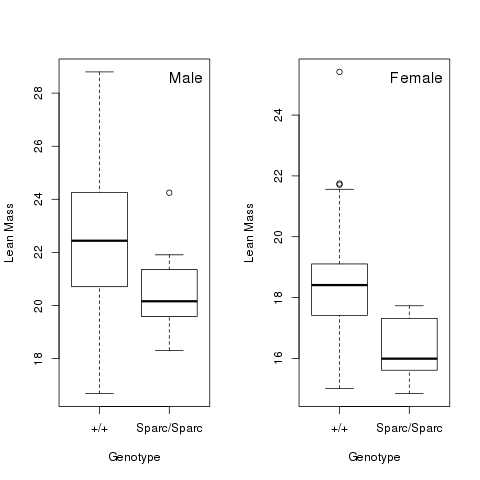
\includegraphics[scale=0.5]{boxplotSexGenotype.png}}
\caption{The PhenStat package's graphical output: box plot split by sex and genotype.}\label{fig:07}
\end{figure}

The example of scatter plot split by sex, genotype and batch is shown in Fig. \ref{fig:08}. This allows a visualisation of variation of dependent variable with time. The MM framework assumes this variation is random and conforms the normal distribution. Then the genotype distribution can be compared relative to natural variation. 
\begin{figure}[!htpb]%figure01
\centerline{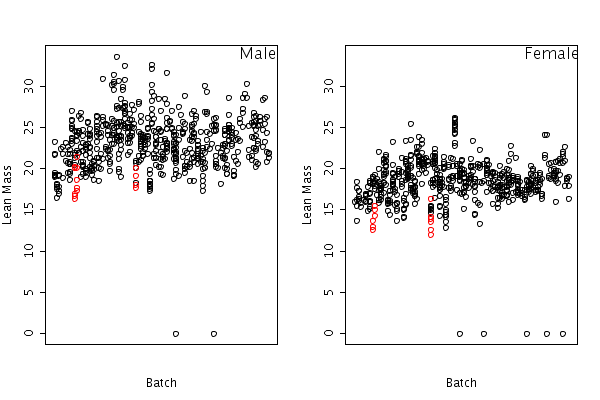
\includegraphics[scale=0.5]{scatterplotSexGenotypeBatch.png}}
\caption{The PhenStat package's graphical output: scatter plot split by sex, genotype and batch.}\label{fig:08}
\end{figure}

The example of scatter plot of body weight versus dependent variable is shown in Fig. \ref{fig:09}. When weight is included in the model MM framework, it assumes a linear relationship between dependent variable and body weight. This graph allows an assessment of this assumption. 
\begin{figure}[!htpb]%figure01
\centerline{\includegraphics[scale=0.5]{scatterplotGenotypeWeight.png}}
\caption{The PhenStat package's graphical output: scatter plot of body weight versus dependent variable.}\label{fig:09}
\end{figure}

\subsubsection{Adjustment for batch}
In order to demonstrate the power of \textit{boxplotSexGenotypeBatchAdjusted} function the following dataset has been used: provided by the Toronto Centre for Phenogenomics of blood plasma calcium data obtained from a study on gene knockout mice carrying the \textit{Tox3 \textsuperscript{tm1b(KOMP)Mbp}} targeted allele which were created by blastocyst injection of targeted ES cells, and bred on the C57BL/6NCrl  genetic background. Data was collected on a standardized high throughput phenotyping pipeline with regular control animals. 

A statistically significant genotype effect was reported from a mixed model analysis of the data (p-value = 6.836e-7) with an estimated effect size of $-0.3535 \pm 007$ mg/dl affecting both sexes equally. However, visually inspection of the raw data suggests that no genotype effect is present (Figure \ref{fig:09a}:A). The conflict arises as the batch differences are masking the genotype effect in the raw data resulting in a boxplot of the raw data where no genotype effect can be observed. It is a strong example of why an analysis that removes batch effects (as the mixed model method does) is needed. The \textit{boxplotSexGenotypeBatchAdjusted} function provides a graphing of the data after modelling has accounted for batch as a random effect and with this approach the genotype effect is then revealed (Figure \ref{fig:09a}:B). It is worth noting that when the graph is plotted with \textit{scatterplotSexGenotypeBatch} function (Figure \ref{fig:09b}) where data is plotted by batch with close inspection the genotype effect can be seen without adjustment.

\begingroup
\fontsize{8pt}{12pt}\selectfont
\begin{verbatim}
> data <- system.file("extdata", "Tox3CaDataset.csv", package="PhenStat")  
> test <- PhenList(dataset=data, testGenotype="heterozygote",	
	 refGenotype="null",dataset.colname.batch="dateOfExperiment",
	 dataset.colname.genotype="zygosity", dataset.colname.sex="sex")
> result <- testDataset(phenList=test, depVariable="dataPoint", equation="withoutWeight", method="MM")
> summaryOutput(result)
> boxplotSexGenotype(test, "dataPoint", "Calcium (mg/dl)")
> boxplotSexGenotypeBatchAdjusted(test, "dataPoint", "Calcium (mg/dl) adjusted for batch")
> scatterplotSexGenotypeBatch(test, "dataPoint", "Calcium (mg/dl)")
\end{verbatim}
\endgroup 

\begin{figure}[!htpb]%figure01
\centerline{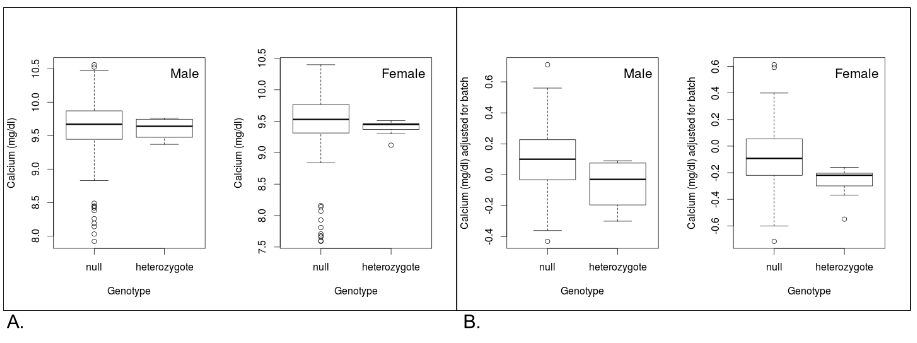
\includegraphics[scale=0.4]{boxplotsBatchEffect.png}}
\caption{Exploration of the variation in calcium with genotype. Data shown is the calcium data for the \textit{Tox3} knockout provided by Toronto Centre for Phenogenomics.
\textbf{A:} \textit{boxplotSexGenotype} function is showing the variation in calcium by sex and genotype. 
\textbf{B:} \textit{boxplotSexGenotypeBatchAdjusted} function is showing the variation in calcium by sex and genotype after removing the effect of batch by modelling batch as a random effect.}\label{fig:09a}
\end{figure}

\begin{figure}[!htpb]%figure01
\centerline{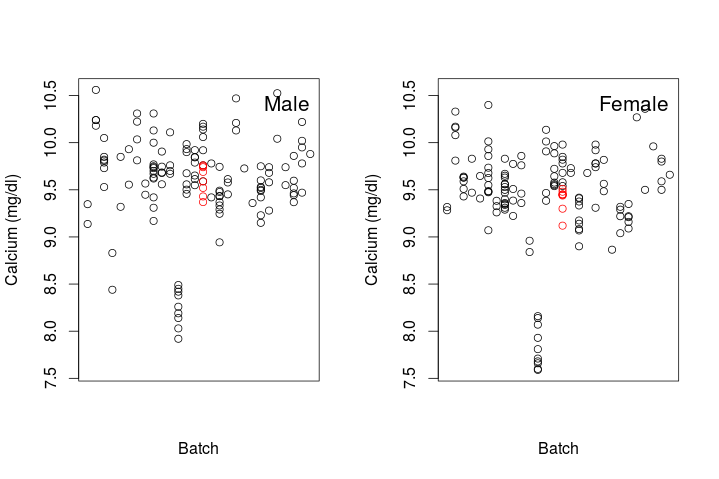
\includegraphics[scale=0.4]{scatterplotBatchEffect.png}}
\caption{Exploration of the variation in calcium with genotype by batch using the function \textit{scatterplotSexGenotypeBatch}. Data shown is the calcium data for the \textit{Tox3} knockout provided by Toronto Centre for Phenogenomics.}\label{fig:09b}
\end{figure}

\subsubsection{Results based graphs}
There are five functions in the results based graphs category:
\begin{itemize}
\item \textit{qqplotGenotype} creates a Q-Q plot of residuals for each genotype.
\item \textit{qqplotRandomEffects} creates a Q-Q plot of blups (best linear unbiased predictions). Only relevant in MM framework.
\item \textit{qqplotRotatedResiduals} creates a Q-Q plot of ``rotated'' residuals.  Only relevant in MM framework.
\item \textit{plotResidualPredicted} creates predicted versus residual values plots split by genotype.
\item \textit{boxplotResidualBatch} creates a box plot with residue versus batch split by genotype.
\end{itemize}


\begingroup
\fontsize{8pt}{12pt}\selectfont
\begin{verbatim}
> qqplotGenotype(result)
# MM framework specific graphic function 
> qqplotRandomEffects(result)
# MM framework specific graphic function 
> qqplotRotatedResiduals(result)
> plotResidualPredicted(result)
> boxplotResidualBatch(result)
\end{verbatim}
\endgroup 

The example of Q-Q plot of residuals for each genotype is shown in Fig. \ref{fig:10}. The MM framework assumes residuals are normally distributed. Residuals are the differences between the real values observed for a dependent variable and the fitted values from the model. A Q-Q plot assesses this assumption (residuals will be randomly arranged around the line if normally distributed). 
\begin{figure}[!tpb]%figure01
\centerline{\includegraphics[scale=0.5]{qqplotGenotype.png}}
\caption{The PhenStat package's graphical output: Q-Q plot of residuals for each genotype.}\label{fig:10}
\end{figure}


The example of Q-Q plot of BLUPs (best linear unbiased predictions) is shown in Fig. \ref{fig:11}. The MM assumes the BLUPs are normally distributed. This graph assesses this assumption by plotting BLUPs and the ideal normal line (large deviations from the line can be an indicator of problems with the model fit). BLUPs are best linear unbiased predictions and are used for the estimation of random batch effects. As such this is specific to MM framework only. See tutorial \href{http://www.extension.org/pages/61006/the-solcap-tomato-phenotypic-data:-estimating-heritability-and-blups-for-traits#.Ui4zjWRgYXc}{BLUPs} for more details.

\begin{figure}[!htpb]%figure01
\centerline{\includegraphics[scale=0.5]{qqplotRandomEffects.png}}
\caption{The PhenStat package's graphical output: Q-Q plot of BLUPs (best linear unbiased predictions).}\label{fig:11}
\end{figure}

Another method to assess the model fit of MM framework is to consider the normality of the ``rotated'' and ``unrotated'' residuals. The example of Q-Q plot of ``rotated'' residuals is shown in Fig. \ref{fig:12}. 
See section \ref{MMDiagnostics} for the details about ``rotated'' residuals.

\begin{figure}[!htpb]%figure01
\centerline{\includegraphics[scale=0.5]{qqplotRotatedResiduals.png}}
\caption{The PhenStat package's graphical output: Q-Q plot of ``rotated'' residuals.}\label{fig:12}
\end{figure}

The example of residual-by-predicted plot is shown in Fig. \ref{fig:13}. Residuals, differences between fitted and real values, are plotted against the predicted (fitted) values of dependent variable.  
A residual-by-predicted plot can be used to diagnose nonlinearity or nonconstant error variance. It is also can be used to find outliers. 

Here are the characteristics of a residual-by-predicted plot when model fitness is close to the ideal and what they suggest about the appropriateness of the model:
\begin{itemize}
\item The residuals are arranged randomly around the 0 line. This suggests that the assumption that the relationship is linear is reasonable.
\item The residuals roughly form a "horizontal band" around the 0 line. This suggests that the variances of the error terms are equal.
\item No one residual outstands from the basic random pattern of residuals. This suggests that there are no outliers. See \href{https://onlinecourses.science.psu.edu/stat501/node/36}{Regression Methods} for more details.
\end{itemize}
\begin{figure}[!htpb]%figure01
\centerline{\includegraphics[scale=0.5]{plotResidualPredicted.png}}
\caption{The PhenStat package's graphical output: residual-by-predicted plot split by genotype.}\label{fig:13}
\end{figure}

The example of box plot with residue versus batch split by genotype is shown in Fig. \ref{fig:14}. This allows assessment that the residual behaviour for all batches is within natural deviation and the model is fitting the data well.
\begin{figure}[!htpb]%figure01
\centerline{\includegraphics[scale=0.5]{boxplotResidualBatch.png}}
\caption{The PhenStat package's graphical output: box plot with residual versus batch split by genotype.}\label{fig:14}
\end{figure}
   
\section{Case Studies}
\subsection{PhenStat MM framework Usage Example}
The following dataset, provided by Wellcome Trust Sanger Institute (WTSI) Mouse Genetics Project (\href{http://www.sanger.ac.uk/resources/mouse/}{MGP}) 
is Dual-energy X-ray absorptiometry data obtained for a study on gene knockout mice carrying the \textit{Akt2$\textless$tm1Wcs$\textgreater$} targeted allele which were created by blastocyst 
injection of targeted ES cells, and bred on the 129S5\//SvEvBrd genetic background.  
Data were collected doing a standardized high throughput phenotyping pipeline following a multi-batch workflow, where regular control animals are collected and knockout animals of the correct age are issued to the pipeline as they arise.  

\begin{table}[!h]
\begin{center}
\begin{tabular}{| l | l | c | c |}
  \hline
Genotype&Sex&Number Animals&Number Batches\\\hline
\multirow{2}{*}{\textit{Akt2}\slash \textit{Akt2}}&Female&12&3\\
			    &Male&14&3\\
			    \hline
\multirow{2}{*}{+\slash +}&Female&574&96\\
			    &Male&572&97\\

\hline  
\end{tabular}
\caption{Number of animals and number of batches in the \textit{Akt2} dataset}\label{table:08}
\end{center}
\end{table}

\subsubsection{Loading the data and initial steps of analysis}
Initial steps focus on loading the data, using the PhenStat tools to generate the PhenList object, and then the result object.  
We can then explore the data and fitted results using the visualisation and output functions. 

  
\begingroup
    \fontsize{8pt}{12pt}\selectfont
\begin{verbatim}
> file <- system.file("extdata", "test_Akt2.csv", package="PhenStat") 
> DEXAdata <- read.csv(file)
> test <- PhenList(dataset=DEXAdata,testGenotype="Akt2/Akt2",  
   refGenotype="WT",
   dataset.colname.batch="dateOfExperiment", 
   dataset.values.female="female", 
   dataset.values.male="male" )
> result <- testDataset(test,depVariable="Lean.Mass",
   method="MM",equation="withoutWeight",transformValues=FALSE)
\end{verbatim}
\endgroup 



\subsubsection{Exploring and understanding the summary output}
\label{cs1_output}
The first two lines of the \textit{summaryOutput} confirm the statistical framework used and the dependent variable studied. If the values of dependent variable have been transformed (see section \ref{section:transformation}) then information about transformation parameters appears together with dependent variable name. For example:
\begingroup
    \fontsize{8pt}{12pt}\selectfont
\begin{verbatim}
> resultTransformed <- testDataset(test,depVariable="Lean.Mass",
   method="MM",equation="withoutWeight",transformValues=TRUE)
> summaryOutput(resultTransformed)

Test for dependent variable:
*** Lean.Mass, power transformed with lambda value = 1.7  and scale shift = 1 ***

Method:
*** Mixed Model framework ***

----------------------------------------------------------------------------
Model Output
----------------------------------------------------------------------------
Final fitted model: Lean.Mass ~ Genotype + Sex
Was batch significant? TRUE
Was variance equal? FALSE
Genotype p-value: 2.661943e-10
Genotype effect (original scale): -10.5581 +/- 2.2910
Was there evidence of sexual dimorphism? no (p-value 1.467981e-01)
Genotype percentage change Female: -30%
Genotype percentage change Male: -21.01%

----------------------------------------------------------------------------
Classification Tag
----------------------------------------------------------------------------
With phenotype threshold value 0.01 - both sexes equally

----------------------------------------------------------------------------
Model Output Summary
----------------------------------------------------------------------------
                      Value Std.Error   DF  t-value       p-value
(Intercept)        92.95823  1.656484 1048 56.11778 4.921042e-318
GenotypeAkt2/Akt2 -27.88930  3.868329 1048 -7.20965  1.072359e-12
SexMale            39.79585  1.243963 1048 31.99118 3.071828e-157
\end{verbatim}
\endgroup 
 
Lean Mass values have been transformed with parameter $\lambda = 1.7$ and parameter $scaleShift = 1$. In the form of equation:
\[
  \text{Lean.Mass}_i = \frac{(\text{Lean.Mass\_original}_i + 1)^{1.7} - 1}{1.7}, \text{for $i = 1, .., 1172$}
\]

The function's \textit{testDataset} output is \textit{PhenTestResult} object that contains slot called \textit{analysedDataset} from which original values (here "Lean.Mass\_original"), transformed values (here "Lean.Mass") and batch adjusted (here "Lean.Mass\_adjusted") values can be obtained:
\begingroup
    \fontsize{8pt}{12pt}\selectfont
\begin{verbatim}
> head(resultTransformed@analysedDataset)
  Lean.Mass    Sex  Genotype                Batch Weight Lean.Mass_original Lean.Mass_adjusted
1  45.34405 Female Akt2/Akt2 2008-10-22T23:00:00Z   14.8              11.98          -5.085269
2  49.13590 Female Akt2/Akt2 2008-03-18T00:00:00Z   17.1              12.60          -6.152621
3  51.26762 Female Akt2/Akt2 2008-03-18T00:00:00Z   17.2              12.94          -5.812621
4  65.58713 Female Akt2/Akt2 2008-03-20T00:00:00Z   18.4              15.09          -4.509509
5  60.56454 Female Akt2/Akt2 2008-03-20T00:00:00Z   18.5              14.36          -5.239509
6  55.24919 Female Akt2/Akt2 2008-10-22T23:00:00Z   18.7              13.56          -3.505269

\end{verbatim}
\endgroup 
Coming back to the output of \textit{summaryOutput} function, the next section of it shows the final fitted model and clarifies model's details. As the MM framework is an optimisation process exploring the data to fit the best model to the data, 
the final fitted model details will vary. We can see that batch variation, the variation in readings between different assay dates, 
were found to be statistical significant ("Was batch significant? TRUE") and hence a mixed model will have been fitted where batch is treated as a random effect.  
If it was not significant, then the model would have reverted to a simpler linear model.  
The next line of output, “Was variance equal?”, indicating whether the model assumes equal variance between genotype groups or unequal.  
In this case, the variance was not found to be equal and therefore the final model estimated the variance for each group separately. 

The “Genotype p-value” reports the statistical significance for the genotype effect and is assessed by comparing a treatment model (final fitted model) with a null model where a null model 
has no genotype effects in the model but all other significant main effects.  
In this example the null model would thus be Lean.Mass $\sim$ Sex.
Looking at the output the "Genotype p-value" is highly statistical significant as a $2.661943e-10$ value is reported. 

After transformation the model estimates are on a new scale and hence for interpretability it is useful to convert these values back to the original scale.  In the \textit{summaryOutput} function, the genotype estimate and standard error is converted and this is reported as “Genotype effect (original scale)”. In our example the genotype effect is estimated at $-10.5581 \pm 2.2910$. 

The next stage of the output, indicates whether there was evidence of sexual dimorphism (i.e. the genotype effect was found to be dependent on sexes).  
In this case, the statistical test of sexual dimorphism was non-significant (p-value = 0.147) hence the final model assessed a genotype effect rather than the genotypes for each sex separately.  

The next two lines of the output show percentage changes --  the ratio of the genotype effect for a sex relative to the wildtype signal for that variable for that sex (see section \ref{section:BiologicalEffect} for more details).
\[
\text{Genotype percentage change Female} = (-27.89/92.96)*100=-30\%
\] 
\[
\text{Genotype percentage change Male} = (-27.89/(92.96+39.8))*100=-21.01\%
\]

As there was no evidence for sexual dimorphism, and thus the genotype effect was estimated independently of sex, then a classification tag “both sexes equally” has been assigned. 

We can then look at the model fitting details in the final output of the function by examining the table to see how the main effects contributed to the variation in the dependent variables. 

A regression model estimates each component of the model, by isolating how that effect influences the dependent variable (i.e. lean mass) as though all other parts of the model had been fixed and isolated.   
From the table of output, we can see that the intercept (the expected reading for lean mass for female reference genotype (aka female wildtype animals) is 92.96.  
Then we can see the effect of the genotype is -27.89 (-10.56 in original scale) in that knockout animals are predicted to have 27.89 grams (10.56 in original scale) less lean mass relative to the control animals.  
Finally we can see that being a male animals leads to an increase of 39.8 grams (11.03 grams in original scale).  
These estimates are in agreement with the visualisation of the data (see section \ref{AssesingModelFit}). 
 
Here is the function example for reverse transformation in order to obtain original scale values: 
\begingroup
    \fontsize{8pt}{12pt}\selectfont
\begin{verbatim}
> reverseTransformValues(c(-27.89,39.8),lambda = 1.7,scaleShift = 1)
[1] -10.55820  11.03411
\end{verbatim}
\endgroup  

Function's \textit{summaryOutput} results for the not transformed lean mass values:
\begingroup
    \fontsize{8pt}{12pt}\selectfont
\begin{verbatim}
> summaryOutput(result)

Test for dependent variable:
*** Lean.Mass ***

Method:
*** Mixed Model framework ***

----------------------------------------------------------------------------
Model Output
----------------------------------------------------------------------------
Final fitted model: Lean.Mass ~ Genotype + Sex
Was batch significant? TRUE
Was variance equal? FALSE
Genotype p-value: 1.901362e-10
Genotype effect: -3.5271 +/- 0.4866
Was there evidence of sexual dimorphism? no (p-value 9.055876e-01)
Genotype percentage change Female: -19.04%
Genotype percentage change Male: -15.24%

----------------------------------------------------------------------------
Classification Tag
----------------------------------------------------------------------------
With phenotype threshold value 0.01 - both sexes equally

----------------------------------------------------------------------------
Model Output Summary
----------------------------------------------------------------------------
                      Value Std.Error   DF   t-value       p-value
(Intercept)       18.525264 0.1936360 1048 95.670550  0.000000e+00
GenotypeAkt2/Akt2 -3.527111 0.4866433 1048 -7.247836  8.204401e-13
SexMale            4.620361 0.1581236 1048 29.219943 8.940893e-138
\end{verbatim}
\endgroup 
\subsubsection{Assessment of raw data and distribution characteristics}
To assess model fit, graphical tools are ideal.  They focus on two areas:
\begin{enumerate}
 \item Assessment of raw data and distribution characteristics
 \item Assessment of model fit
\end{enumerate}
\label{AssesingModelFit}

The function, \textit{boxplotSexGenotype}, allows the genotype effect to be visualised for each sex group. 
For the \textit{Akt2} example, we can suggest that there looks to be a significant genotype effect that is seen in both sexes. 


\begingroup
    \fontsize{8pt}{12pt}\selectfont
\begin{verbatim}
> boxplotSexGenotype(result, "Lean.Mass", "Lean Mass (g)")
\end{verbatim}
\endgroup 

\begin{figure}[H]%figure01
\centerline{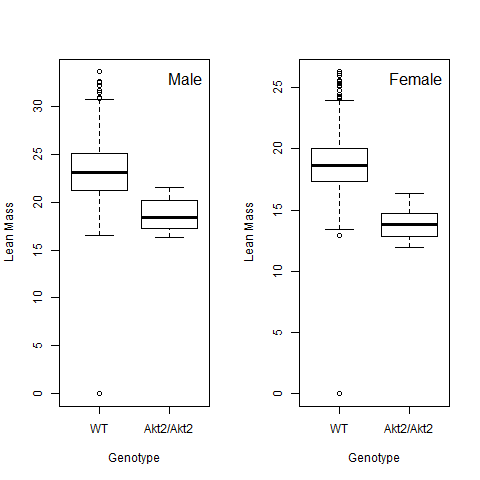
\includegraphics[scale=0.5]{cs1_boxplotSexGenotype.png}}
\caption{\textit{boxplotSexGenotype} function for \textit{Akt2} example.}\label{fig:15}
\end{figure}

A second function, \textit{scatterplotSexGenotypeBatch}, allows the comparison between genotype as a function of batch and sex.  
This plot allows the user to visualise the batch variation and assess how the treatment measures look relative to the batch variation. 
It is important to note that as dates can be entered in many forms, the batches are not ordered with time. 
For the \textit{Akt2} lean mass example, we can see that there is significant batch variation, which explains why a mixed model was fitted.

\begingroup
    \fontsize{8pt}{12pt}\selectfont
\begin{verbatim}
> scatterplotSexGenotypeBatch(test, "Lean.Mass", "Lean Mass (g)")
\end{verbatim}
\endgroup 

\begin{figure}[H]%figure01
\centerline{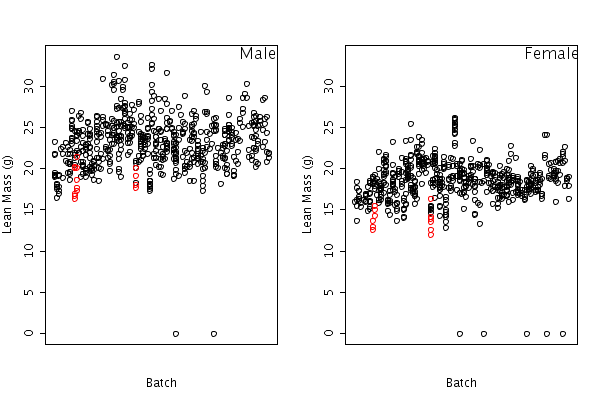
\includegraphics[scale=0.5]{cs1_scatterplotSexGenotypeBatch.png}}
\caption{\textit{scatterplotSexGenotypeBatch} function for \textit{Akt2} example.}\label{fig:16}
\end{figure}

\subsubsection{Assessment of model fit}

Five functions are available and they focus on looking at residual behaviour. 
A residual, is the difference between the estimated dependent variable from the final model estimates and the actual measured dependent variable response. 
A model is a good fit, when the residuals are normally distributed and there is no systematic pattern in the distribution of the residuals relative to the dependent variable. 

The \textit{vectorOutput} function includes statistical tests for normality on the residuals for the wildtype, residuals for the knockout, the blups and ``rotated'' residuals (see section \ref{MMDiagnostics}). 
These normality tests are provide to assist in the building automated tools for assessing model fit, 
however when there is a lot of data (e.g. in a dataset where the wildtype arises from a high throughput program with a running baseline), 
the statistical test can be overall sensitive to departures from normality and when the number of data points is low (e.g. in many knockout groups), the test can lack ability to detect deviations from normality. 

\begin{itemize}
 \item \textbf{qqplotGenotype} 
 
This function assesses the normality of the residuals are assessed for each genotype through plotting a normal Q-Q plot. 
Q-Q plots are a means of comparing two distributions. To test normality, we plot the residuals against a normal distribution and see if they match. 
If the two distributions are similar the points on a QQ plot will fall along the y=x line (unity). Thus we are looking for a random distribution of points along the lines.  

Looking at the \textit{Akt2} lean mass example, the residuals on the homozygous knockout group are near perfect showing the model is fitting this data well.  
The residuals on the WT group are deviating in a way (systematic below at one end and systematic above at the other) which indicates that we have long tails to our distribution. 
This is not concerning as we have a very large control dataset and we do have outliers in the data.  

\begingroup
    \fontsize{8pt}{12pt}\selectfont
\begin{verbatim}
> qqplotGenotype(result)
\end{verbatim}
\endgroup 

\begin{figure}[H]%figure01
\centerline{\includegraphics[scale=0.5]{cs1_qqplotGenotype.png}}
\caption{\textit{qqplotGenotype} function for \textit{Akt2} example.}\label{fig:17}
\end{figure}

\item \textbf{boxplotResidualBatch} 

This function allows visualisation to assist the user to assess whether the deviation in the residual is consistent across all the batches and similar in size between the wildtype and knockout line. 
For the \textit{Akt2} example, we can see that the variation in residual is consistent across all the batches and similar in size between the knockout and wildtype group.

A few of the wildtype (control) dataset points have large residuals and it would be worth looking at these data points further to see why these are outliers. They do not suggest the model should be discarded because as a proportion of the dataset they are few and scattered through the dataset.

\begingroup
    \fontsize{8pt}{12pt}\selectfont
\begin{verbatim}
> boxplotResidualBatch(result)
\end{verbatim}
\endgroup 

\begin{figure}[H]%figure01
\centerline{\includegraphics[scale=0.5]{cs1_boxplotResidualBatch.png}}
\caption{\textit{boxplotResidualBatch} function for \textit{Akt2} example.}\label{fig:18}
\end{figure}


\item \textbf{plotResidualPredicted} 

This function plots the residuals against the predicted readings for both genotypes.  The predicted readings are the values the model would estimate for the dependent variable.  
As a user, you are looking to see that the model is fitting the data well over the entire data range. 
Looking at the \textit{Akt2} data, we can see that there spread of the residuals is fairly consistent, 
however there are some data points that are not being fit well by the model, the good news is that they are in the control set but they should be considered further to see if a reason for their poor fit can be ascertained.  

\begingroup
    \fontsize{8pt}{12pt}\selectfont
\begin{verbatim}
> plotResidualPredicted(result)
\end{verbatim}
\endgroup 

\begin{figure}[H]%figure01
\centerline{\includegraphics[scale=0.5]{cs1_plotResidualPredicted.png}}
\caption{\textit{plotResidualPredicted} function for \textit{Akt2} example.}\label{fig:19}
\end{figure}

\item \textbf{qqplotRandomEffects} 

This function is assessing the assumption that the batch effects are normally distributed. 
The estimates of the random effects, aka the estimates of the batch effects in this scenario, are called best linear unbiased prediction BLUPs. 
Here a normal Q-Q plot is used to plot the estimated BLUPs against a normal distribution. 
So looking at the \textit{Akt2} lean mass example, the majority of the data points are distrbuted along the line. 
There is some systematic deviation at the tails but it is a small percentage of the points and as it is above and below the line it indicates long tails (ie outliers) 
and so we can conclude the distribution is not too far from the ideal and the model is a good representation of the data. 

\begingroup
    \fontsize{8pt}{12pt}\selectfont
\begin{verbatim}
> qqplotRandomEffects(result)
\end{verbatim}
\endgroup 

\begin{figure}[H]%figure01
\centerline{\includegraphics[scale=0.5]{cs1_qqplotRandomEffects.png}}
\caption{\textit{qqplotRandomEffects} function for \textit{Akt2} example.}\label{fig:20}
\end{figure}

\item \textbf{qqplotRotatedResiduals}

This function, allows the user to consider the normality of the ``rotated'' and ``unrotated'' residuals and have been recommended to assess model fit success with mixed models (\cite{RotatedResiduals04}). 
See section \ref{MMDiagnostics} for more details. 
So looking at the \textit{Akt2} lean mass example, the majority of the data points are distributed along the line. 
There is some systematic deviation at the tails but it is a small percentage of the points and as it is above and below the line it indicates long tails (i.e. outliers) 
and so we can conclude the distribution is not too far from the ideal and the model is a good representation of the data. 

\begingroup
    \fontsize{8pt}{12pt}\selectfont
\begin{verbatim}
> qqplotRotatedResiduals(result)
\end{verbatim}
\endgroup 

\begin{figure}[H]%figure01
\centerline{\includegraphics[scale=0.5]{cs1_qqplotRotatedResiduals.png}}
\caption{\textit{qqplotRotatedResiduals} function for \textit{Akt2} example.}\label{fig:21}
\end{figure}
\end{itemize}

\subsubsection{Including weight as a covariate in the model fitting process}
Weight is included in the initial model via the \textit{testDataset} function equation argument being set to either “withWeight” or “withoutWeight”.  
When weight is included as a covariate, the model is assuming that the dependent variable (e.g. lean mass) has a linear relationship with body weight. 
If weight is not found to be statistical significant in explaining the variation in the dependent variable, 
then weight as a covariate will drop out of the final model and the equation will automatically revert to an equation type “withoutWeight”.  

There are two advantages to including weight:
\begin{enumerate}
 \item \textbf{Increase in sensitivity.}  
If differences in animal weight lead to greater variability in the dependent variable, then by adding weight and accounting for this variability then the statistical model will be more sensitive to a genotype effect. 

 \item \textbf{Adjusting for weight differences between the knockout and control group.}  
When there is a weight difference between the knockout and wildtype animals, the genotype effect is confounded by the weight effect in that there is a difference in the dependent variable but you cannot assess whether it is due to the differences in body weight of the knockout and control animals or genotype differences between the knockout and control animals. When weight is included in the equation, the genotype effect is then testing for a genotype difference after adjusting for the weight difference.

\end{enumerate}

We have found that the majority of continuous phenotypic variables monitored in the WTSI Mouse Genetics Project (\href{http://www.sanger.ac.uk/resources/mouse/}{MGP}) have a relationship with body weight. 
Looking at the \textit{Akt2} dataset we can see that there is a difference in body weight between the wildtype and knockout group and thus body weight can be a confounding factor to isolating the genotype effect.   

\begingroup
    \fontsize{8pt}{12pt}\selectfont
\begin{verbatim}
> boxplotSexGenotype(test, "Weight", "Body Weight (g)")
\end{verbatim}
\endgroup 

\begin{figure}[H]%figure01
\centerline{\includegraphics[scale=0.5]{cs1_bodyweight.png}}
\caption{\textit{boxplotSexGenotype} function for \textit{Akt2} example to show the body weight impact.}\label{fig:22}
\end{figure}

When body weight is included, the inclusion can be seen in the final fitted model as weight is listed as a covariate and then in the final model output table, where the influence of weight on the fitted model is shown.  
With weight included the genotype effect is estimating the impact of genotype after adjusting for weight differences in the animals. 

Looking at the \textit{summaryOutput} for the \textit{Akt2} example, the table shows that for each gram of body weight the lean mass increased by 0.32g.  
When weight is included in the equation it changes the definition of the intercept from the lean mass value of a wildtype female animal to the lean mass value of a wildtype female animal of zero body weight. 
This happens as the model is estimating each of these terms influences in isolation of the other terms. 
In contrast to the earlier fitted results (section \ref{cs1_output}), when weight is included in the model, the classification tag identifies the change as “no significant change” 
as the global genotype test is now not significant with a p-value of 0.64.  
This means the statistically difference observed with the fitted model “withoutWeight” was entirely due to a body weight differences between the knockout and control animals.  
So whilst there is a fundamental differences in lean mass between the knockout and control this is due to the knockout animals being smaller than the control animals. 

\begingroup
    \fontsize{8pt}{12pt}\selectfont
\begin{verbatim}
> result <- testDataset(test,depVariable="Lean.Mass",
   method="MM",equation="withWeight",transformValues=FALSE)
> summaryOutput(result)

Test for dependent variable:
*** Lean.Mass ***

Method:
*** Mixed Model framework ***

----------------------------------------------------------------------------
Model Output
----------------------------------------------------------------------------
Final fitted model: Lean.Mass ~ Genotype + Sex + Weight
Was batch significant? TRUE
Was variance equal? FALSE
Genotype p-value: 6.399898e-01
Genotype effect: -0.1925 +/- 0.4120
Was there evidence of sexual dimorphism? no (p-value 1.053833e-01)
Genotype percentage change Female: -1.04%
Genotype percentage change Male: -0.83%

----------------------------------------------------------------------------
Classification Tag
----------------------------------------------------------------------------
With phenotype threshold value 0.01 - no significant change

----------------------------------------------------------------------------
Model Output Summary
----------------------------------------------------------------------------
                       Value  Std.Error   DF    t-value      p-value
(Intercept)        7.6201046 0.52150631 1047 14.6117207 3.827390e-44
GenotypeAkt2/Akt2 -0.1924952 0.41201772 1047 -0.4672012 6.404531e-01
SexMale            2.1550868 0.17386173 1047 12.3954067 5.056608e-33
Weight             0.3541522 0.01623164 1047 21.8186332 2.718321e-87
\end{verbatim}
\endgroup


\subsubsection{Additional model diagnostics when weight is included}
In addition to the diagnostic discussed in previous section, when weight is included in the model, it is important to consider whether the linear relationship between body weight and the dependent variable is a valid assumption. 
This can be assessed with the \textit{scatterplotGenotypeWeight} function. 
In this plot, for each genotype a regression line is fitted to assess the relationship between the dependent variable and body weight. 
Then a locally weight line (loess line) is plotted. 
The loess line allows assessment that the regression line fits all the data well.
Note the loess line can be distorted by a few data points so if it deviates strongly but for only a few data points, this is not concerning.  
This graph is used to assess whether a linear relationship exists and whether it is the same for both genotypes.  

In the \textit{Akt2} example, it can be clearly seen that a common linear relationship exists between lean mass and body weight, such that as the weight increases so does the lean mass. 
It can also be seen that the knockout animals have a lower body weight and subsequently lower lean mass but the drop in lean mass is entirely in accordance with the drop in body weight. 

\begingroup
\fontsize{8pt}{12pt}\selectfont
\begin{verbatim}
> scatterplotGenotypeWeight(test, depVariable="Lean.Mass")
\end{verbatim}
\endgroup 

\begin{figure}[H]%figure01
\centerline{\includegraphics[scale=0.5]{cs1_scatterplotGenotypeWeight.png}}
\caption{\textit{scatterplotGenotypeWeight} function for \textit{Akt2} example.}\label{fig:23}
\end{figure}

\subsection{PhenStat TF framework Usage Example}
\label{cs_tf}
The following dataset, provided by the German Mouse Clinic  from a plasma chemistry study on gene knockout mice carrying the \textit{Dbn1} targeted allele on the C57BL\//6NTac(USA) genetic background. Data was collected via a standardised high throughput phenotyping pipeline following a multi-batch workflow, with concurrent controls.  The dataset contains baseline controls of which a proportion is concurrent.

\begin{table}[!h]
\begin{center}
\begin{tabular}{| l | l | c | c |}
  \hline
Genotype&Sex&Number Animals&Number Batches\\\hline
\multirow{2}{*}{Het}&Female&9&3\\
			    &Male&10&3\\
			    \hline
\multirow{2}{*}{WT(concurrent controls)}&Female&6&1\\
			    &Male&10&3\\
\multirow{2}{*}{WT(baseline controls)}&Female&189&NA\\
			    &Male&218&NA\\
\hline  
\end{tabular}
\caption{Number of animals and number of batches in the \textit{Dbn1} dataset}\label{table:08_tf}
\end{center}
\end{table}

\subsubsection{Loading the data and initial steps of analysis}
Initial steps focus on loading the data ready for statistical analysis. For the TF framework there are two steps; first the use of PhenList and a second specific function to the TF framework using the \textit{TFDataset} function to generate a dataset cleaned to remove control data that isn’t concurrent.  The resulting cleaned data can be analysed and the results explored using the visualisation and output functions. 
 
\begingroup
\fontsize{8pt}{12pt}\selectfont
\begin{verbatim}
>file <- system.file("extdata", "test7_TFE.csv", package="PhenStat") 

>test <- PhenList(dataset=read.csv(file), refGenotype="WT", testGenotype="het",
dataset.colname.sex="sex", dataset.values.male="m",dataset.values.female="f",
dataset.colname.batch="Date_of_procedure_start",dataset.colname.weight="body.weight")
...
>testTF_new <- TFDataset(test,depVariable="HDL")
Data points containing 'HDL' by batch levels:
|  ----------- |  ----------- |  ----------- |  ----------- |  ----------- |
|              |           WT |           WT |          het |          het |
|  ----------- |  ----------- |  ----------- |  ----------- |  ----------- |
|        Batch |       Female |         Male |       Female |         Male |
|  ----------- |  ----------- |  ----------- |  ----------- |  ----------- |
| * 02.09.2013 |            7 |            4 |            0 |            0 |
|  ----------- |  ----------- |  ----------- |  ----------- |  ----------- |
| * 03.02.2014 |            0 |            1 |            0 |            0 |
|  ----------- |  ----------- |  ----------- |  ----------- |  ----------- |
| * 03.03.2014 |            6 |            6 |            0 |            0 |
|  ----------- |  ----------- |  ----------- |  ----------- |  ----------- |
...
|  ----------- |  ----------- |  ----------- |  ----------- |  ----------- |
| * 14.01.2014 |            5 |            7 |            0 |            0 |
|  ----------- |  ----------- |  ----------- |  ----------- |  ----------- |
|   14.04.2014 |            0 |            4 |            4 |            3 |
|  ----------- |  ----------- |  ----------- |  ----------- |  ----------- |
| * 14.10.2013 |            7 |            5 |            0 |            0 |
|  ----------- |  ----------- |  ----------- |  ----------- |  ----------- |
| * 15.07.2013 |            5 |            5 |            0 |            0 |
|  ----------- |  ----------- |  ----------- |  ----------- |  ----------- |
| * 16.06.2014 |            8 |            8 |            0 |            0 |
|  ----------- |  ----------- |  ----------- |  ----------- |  ----------- |
| * 16.09.2013 |            2 |            3 |            0 |            0 |
|  ----------- |  ----------- |  ----------- |  ----------- |  ----------- |
|   17.02.2014 |            6 |            4 |            3 |            4 |
|  ----------- |  ----------- |  ----------- |  ----------- |  ----------- |
| * 17.03.2014 |            4 |            5 |            0 |            0 |
|  ----------- |  ----------- |  ----------- |  ----------- |  ----------- |
|   18.02.2014 |            0 |            3 |            2 |            3 |
|  ----------- |  ----------- |  ----------- |  ----------- |  ----------- |
| * 18.03.2014 |            4 |            3 |            0 |            0 |
|  ----------- |  ----------- |  ----------- |  ----------- |  ----------- |
...
|  ----------- |  ----------- |  ----------- |  ----------- |  ----------- |
| * 31.03.2014 |            3 |            3 |            0 |            0 |
|  ----------- |  ----------- |  ----------- |  ----------- |  ----------- |
* - removed record(s)

Number of batch levels left: 3
Records removed (reference genotype): 92%
Records removed (test genotype): 0%

>result <- testDataset(testTF_new, depVariable="HDL", dataPointsThreshold=2, method="TF",
transformValues=FALSE) 
...
\end{verbatim}
\endgroup 

The cleaning of the data is reported in the output of the \textit{TFDataset} function.  First the output shows the number of data points by batch for each sex and genotype combination.  For data to be retained for a date, there needs to be both test and ref genotype data for a sex. Summary statistics on the cleaning impact are then provided following the table of data.  

\subsubsection{Exploring and understanding the summary output}
The first two lines of the \textit{summaryOutput} confirm the statistical framework used and the dependent variable studied. The next section of the output clarifies the final fitted model details. As the TF framework is an optimisation process exploring the data to fit the best model to the data, the final fitted model details will vary. We can see that batch variation, the variation in readings between different assay dates, were found to be statistical significant and hence a model including batch as a fixed effect was fitted.  The next line of output, “Was variance equal?", indicating whether the model assumes equal variance between genotype groups or unequal. In this case, the variance was not found to be equal and therefore the final model estimated the variance for each group separately.

Furthermore, we can see that there was statistical evidence of sexual dimorphism and therefore the final model would estimate the genotype effect for each sex separately. The next stage of the output, classification tag, details the classification of the effect seen as discussed in section \ref{TF_classificationTag} and in this case the genotype effect was specific to the males at the default (0.01) threshold. 

\begingroup
\fontsize{8pt}{12pt}\selectfont
\begin{verbatim}
>summaryOutput(result)

Test for dependent variable:
*** HDL ***

Method:
*** Time as Fixed Effect framework ***

----------------------------------------------------------------------------
Model Output
----------------------------------------------------------------------------
Final fitted model: HDL ~ Sex + Genotype:Sex + Weight + Batch
Was batch significant? TRUE
Was variance equal? FALSE
Genotype p-value: 1.072892e-04
Genotype by male effect: -0.3063 +/- 0.0781
Genotype by female effect: -0.0170 +/- 0.0856
Was there evidence of sexual dimorphism? yes (p-value 3.044927e-02)
Genotype percentage change Female: -1.44%
Genotype percentage change Male: -19.15%

----------------------------------------------------------------------------
Classification Tag
----------------------------------------------------------------------------
With phenotype threshold value 0.01 - males only

----------------------------------------------------------------------------
Model Output Summary
----------------------------------------------------------------------------
                            Value  Std.Error    t-value      p-value
(Intercept)            0.18543523 0.24670119  0.7516593 4.583132e-01
SexMale                0.15246298 0.07485017  2.0369090 5.087890e-02
Weight                 0.05286366 0.01036426  5.1005716 1.917964e-05
Batch17.02.2014       -0.25235168 0.05892587 -4.2825277 1.848788e-04
Batch18.02.2014       -0.48135264 0.06644529 -7.2443452 5.617868e-08
SexFemale:Genotypehet -0.01704878 0.08560398 -0.1991587 8.435284e-01
SexMale:Genotypehet   -0.30625701 0.07813579 -3.9195486 4.975257e-04
\end{verbatim}
\endgroup 

We can also see in this section the assessment of the “Genotype p-value" reports the statistical significance for the genotype effect and is assessed by comparing a treatment model (final fitted model) with a null model where a null model has no genotype effects in the model but all other significant main effects. 

In this example the null model would thus be $HDL \backsim Sex + Weight + Batch$. Looking at the output the “Genotype p-value" is statistical significant as a 0.0001 value is reported. 

The percentage changes --  the ratio of the genotype effect for a sex relative to the wildtype signal for that variable for that sex (see section \ref{section:BiologicalEffect} for more details) are estimated as -1.44\% for females and -19.15\% for males.

There was an evidence for sexual dimorphism, so according to the decision tree from Figure \ref{fig:05} the classification tag "males only" has been assigned.

The final section of the output "Model Output Summary" provides a summary table showing the estimates for each component of the final model fitted. As a regression model estimates each component of the model, by isolating how that effect influences the dependent variable (i.e. HDL) as though all other parts of the model had been fixed and isolated. From the summary output, we can see that the intercept (the expected reading for HDL) for female reference genotype (aka female wildtype animals of 0 body weight for the first batch) is 0.185. Then we can see that being male is statistical significant and leads to an increase in HDL of 0.152.  We can also see the impact of weight 0.0528\//g.  As batch was significant source of variation, and it is treated as a fixed effect we can see the estimated impact of each batch on the readings.  Finally, we can see the impact of being het male mouse where the values were lower by -0.3 units with standard error of 0.078.  The lack of significance of the female het mice can be seen in that the estimated effect is -0.02 with an error term 0.09 which is larger than the estimated effect and therefore this effect cannot be classed as significant.

\subsubsection{Assessment of raw data and distribution characteristics}
Graph of the knockout data against the baseline controls:

\begingroup
\fontsize{8pt}{12pt}\selectfont
\begin{verbatim}
> boxplotSexGenotype(test, "HDL", "High Density Lipoprotein (mM)")
\end{verbatim}
\endgroup 

\begin{figure}[H]%figure01
\centerline{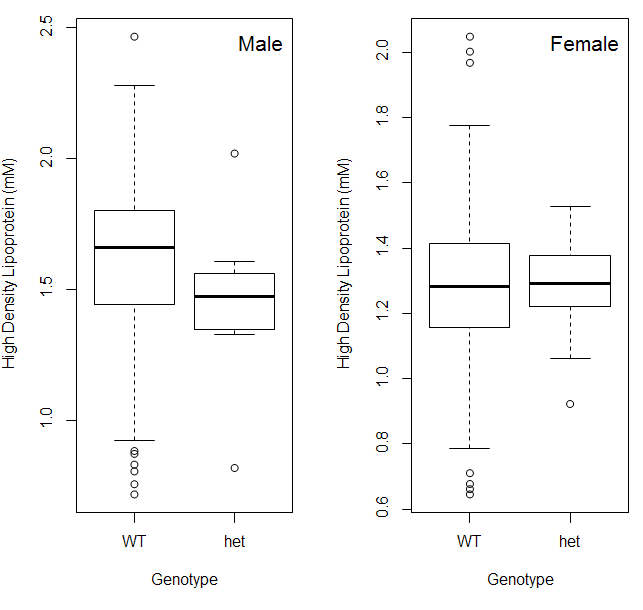
\includegraphics[scale=0.5]{cs_tf_1.jpg}}
\caption{\textit{boxplotSexGenotype} for the \textit{Dbn1} High Density Lipoprotein example showing the baseline and concurrent controls.}\label{fig:cs_tf1}
\end{figure}

Graph of the knockout versus the concurrent controls:
 
\begingroup
\fontsize{8pt}{12pt}\selectfont
\begin{verbatim}
> boxplotSexGenotype(testTF_new, "HDL", "High Density Lipoprotein (mM)")
\end{verbatim}
\endgroup 

\begin{figure}[H]%figure01
\centerline{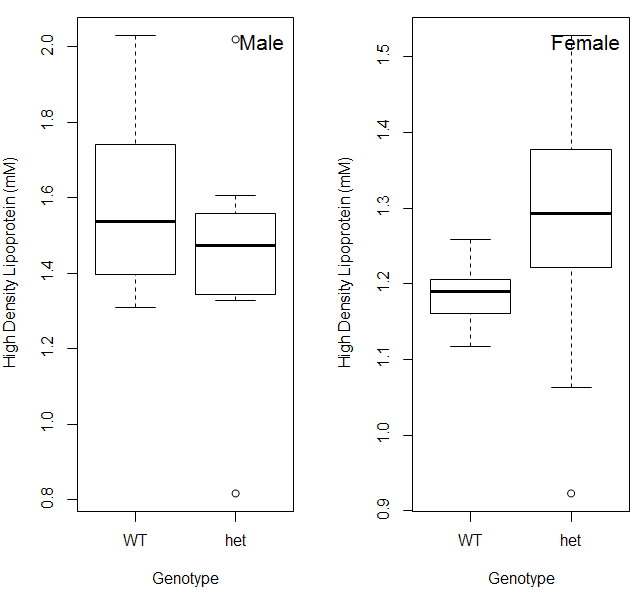
\includegraphics[scale=0.5]{cs_tf_2.jpg}}
\caption{\textit{boxplotSexGenotype} for the \textit{Dbn1} High Density Lipoprotein example showing only the concurrent controls.}\label{fig:cs_tf2}
\end{figure}

Graph showing batch variation for the baseline and concurrent controls:
\begingroup
\fontsize{8pt}{12pt}\selectfont
\begin{verbatim}
> scatterplotSexGenotypeBatch(test, "HDL", "High Density Lipoprotein (mM)")
\end{verbatim}
\endgroup 

\begin{figure}[H]%figure01
\centerline{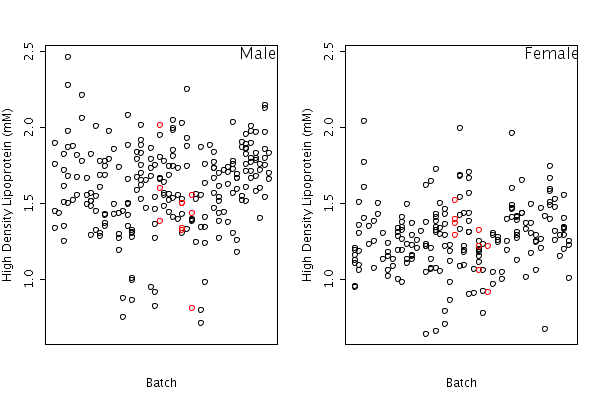
\includegraphics[scale=0.5]{cs_tf_3.png}}
\caption{\textit{scatterplotSexGenotypeBatch} for the \textit{Dbn1} High Density Lipoprotein example showing the baseline and concurrent controls. The test genotype \textit{Dbn1} data are highlighted with red colour.}\label{fig:cs_tf3}
\end{figure}

Graph showing batch variation for the concurrent controls only:
\begingroup
\fontsize{8pt}{12pt}\selectfont
\begin{verbatim}
> scatterplotSexGenotypeBatch(testTF_new, "HDL", "High Density Lipoprotein (mM)")
\end{verbatim}
\endgroup 

\begin{figure}[H]%figure01
\centerline{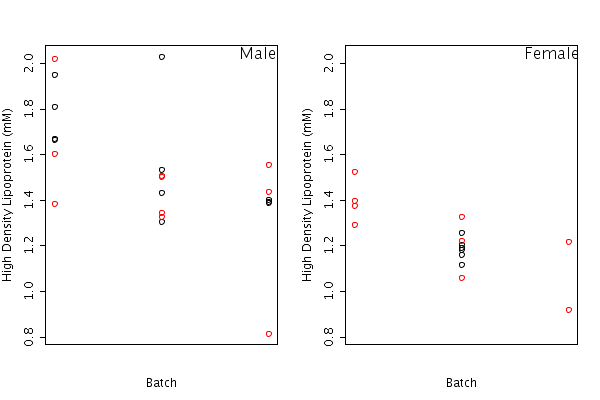
\includegraphics[scale=0.5]{cs_tf_4.png}}
\caption{\textit{scatterplotSexGenotypeBatch} for the \textit{Dbn1} High Density Lipoprotein example showing the concurrent controls. The test genotype \textit{Dbn1} data are highlighted with red colour.}\label{fig:cs_tf4}
\end{figure}

\subsubsection{Assessment of model fit}
Three functions are available and they focus on looking at residual behaviour. The mixed model methodology has an additional two (\textit{qqplotRandomEffects} and \textit{qqplotRotatedResiduals}) which are not relevant to this framework as they assess the assumptions around batch when treated as a random effect. A residual, is the difference between the estimated dependent variable from the final model estimates and the actual measured dependent variable response. A model is a good fit, when the residuals are normally distributed and there is no systematic pattern in the distribution of the residuals relative to the dependent variable.

The \textit{vectorOutput} function includes statistical tests for normality on the residuals for the wildtype and residuals for the knockout (see section \ref{section:vectorOutput}). These normality tests are provide to assist in the building automated tools for assessing model fit, however when there is a lot of data (e.g. in a dataset where the wildtype arises from a high throughput program with a running baseline), the statistical test can be overall sensitive to departures from normality and when the number of data points is low (e.g. in many knockout groups), the test can lack ability to detect deviations from normality.

\begin{itemize}
\item \textbf{qqplotGenotype} 

This function assesses the normality of the residuals are assessed for each genotype through plotting a normal Q-Q plot. Q-Q plots are a means of comparing two distributions. To test normality, we plot the residuals against a normal distribution and see if they match. If the two distributions are similar the points on a QQ plot will fall along the y=x line (unity). Thus we are looking for a random distribution of points along the lines. Looking at the \textit{Dbn1} High Density Lipoprotein example, the residuals on the both the wildtype and heterozygous knockout group are near perfect showing the model is fitting this data well. 

\begingroup
\fontsize{8pt}{12pt}\selectfont
\begin{verbatim}
> qqplotGenotype(result)
\end{verbatim}
\endgroup 

\begin{figure}[H]%figure01
\centerline{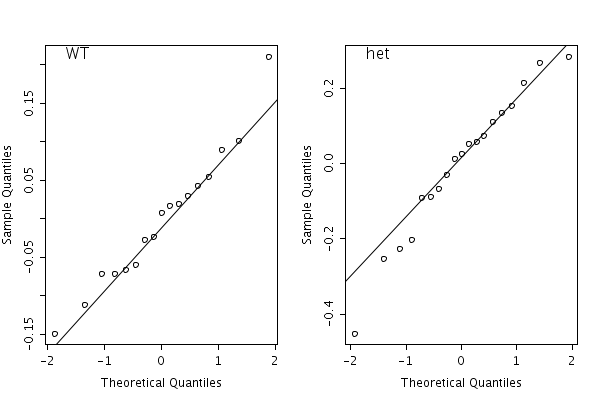
\includegraphics[scale=0.5]{cs_tf_5.png}}
\caption{\textit{qqplotGenotype} function for \textit{Dbn1} High Density Lipoprotein example.}\label{fig:cs_tf5}
\end{figure}

\item \textbf{boxplotResidualBatch} 

This function allows visualisation to assist the user to assess whether the deviation in the residual is consistent across all the batches and similar in size between the wildtype and knockout line. For the \textit{Dbn1} High Density Lipoprotein example, we can see that the variation in residual is consistent across all the batches.  It is higher in the knockout dataset which is why the final fitted model did not assume equal variance.  

\begingroup
\fontsize{8pt}{12pt}\selectfont
\begin{verbatim}
> boxplotResidualBatch(result)
\end{verbatim}
\endgroup 

\begin{figure}[H]%figure01
\centerline{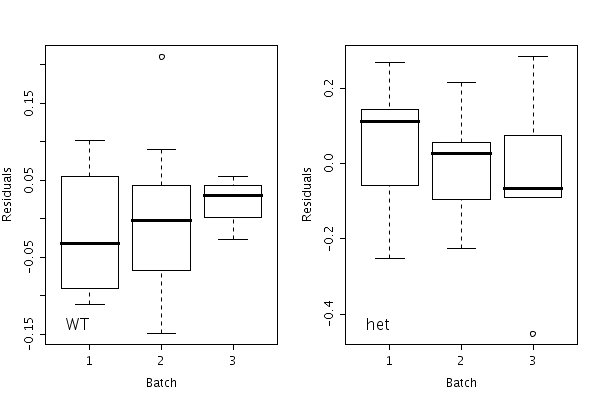
\includegraphics[scale=0.5]{cs_tf_6.png}}
\caption{\textit{boxplotResidualBatch} function for \textit{Dbn1} High Density Lipoprotein example.}\label{fig:cs_tf6}
\end{figure}


\item \textbf{plotResidualPredicted} 

This function plots the residuals against the predicted readings for both genotypes. The predicted readings are the values the model would estimate for the dependent variable. As a user, you are looking to see that the model is fitting the data well over the entire data range. Looking at the \textit{Dbn1} High Density Lipoprotein data, we can see that there spread of the residuals is fairly consistent, suggesting the model is a good fit for all the data points. 

\begingroup
    \fontsize{8pt}{12pt}\selectfont
\begin{verbatim}
> plotResidualPredicted(result)
\end{verbatim}
\endgroup 

\begin{figure}[H]%figure01
\centerline{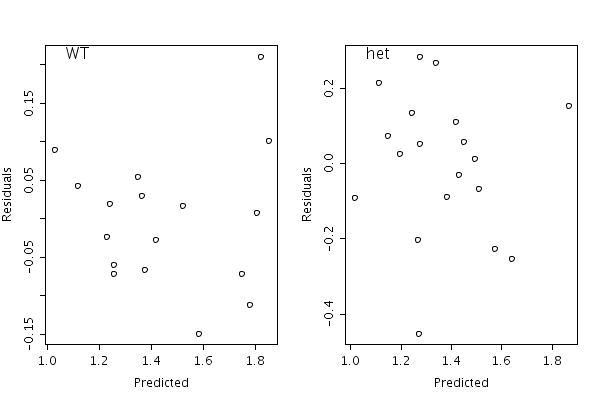
\includegraphics[scale=0.5]{cs_tf_7.png}}
\caption{\textit{plotResidualPredicted} function for \textit{Dbn1} High Density Lipoprotein example.}\label{fig:cs_tf7}
\end{figure}
\end{itemize}

\subsection{PhenStat RR framework Usage Example}
The following dataset, provided by Wellcome Trust Sanger Institute (WTSI) Mouse Genetics Project (MGP) is Dual-energy X-ray absorptiometry data obtained for a study on gene knockout mice carrying \textit{Akt2$\textless$tm1Wcs$\textgreater$} targeted allele which were created by blastocyst injection of targeted ES cells, and bred on the 129S5\//SvEvBrd genetic background. Data was collected doing a standardized high throughput phenotyping pipeline following a multi-batch workflow, where regular control animals are collected and knockout animals of the correct age are issued to the pipeline as they arise. 

See Table \ref{table:08}.

\subsubsection{Loading the data and initial steps of analysis}
Initial steps focus on loading the data, using the PhenStat tools to generate the PhenList object, and then the result object. We can then explore the data and fitted results using the visualisation and output functions.


\begingroup
\fontsize{8pt}{12pt}\selectfont
\begin{verbatim}
> file <- system.file("extdata", "test_Akt2.csv", package="PhenStat") 
> DEXAdata <- read.csv(file)
> test <- PhenList(dataset=DEXAdata,
		  testGenotype="Akt2/Akt2",
		  refGenotype="WT",
		  dataset.colname.batch="dateOfExperiment",
		  dataset.values.female="female",
		  dataset.values.male="male", 
		  dataset.colname.genotype="Genotype", 
		  dataset.colname.sex="Gender")
> result <- testDataset(test, 
			depVariable="Lean.Mass", 
			method="RR")
\end{verbatim}
\endgroup 

\subsubsection{Visualisation of data}
The function \textit{categoricalBarplot} has been provided to visualise the categorical data formed from the RR framework as summary percentage data. It reports the percentage of each classification observed for up to three datasets: all data, male only and female only. It is important to note that percentage accuracy is very dependent on the number of readings so it is important to consider the dataset size when interpreting these graphs. Therefore tables showing both the percentage and count values are included in the \textit{summaryOutput}.


\begingroup
    \fontsize{8pt}{12pt}\selectfont
\begin{verbatim}
> categoricalBarplot(result)
\end{verbatim}
\endgroup 

\begin{figure}[H]%figure01
\centerline{\includegraphics[scale=0.5]{RR_graph.png}}
\caption{\textit{categoricalBarplot} function for \textit{Akt2} Lean Mass example.}\label{fig:16a}
\end{figure}


\subsubsection{Understanding the summaryOutput}

\begingroup
    \fontsize{8pt}{12pt}\selectfont
\begin{verbatim}
> summaryOutput(result)

Test for dependent variable:
*** Lean.Mass ***

Method:
*** Reference Ranges Plus framework ***

1) High vs Normal/Low
           All Females only Males only
p-value 1.0000       1.0000     1.0000
ES          3%           3%         3%

2) Low vs Normal/High
           All Females only Males only
p-value 0.0000       0.0000     0.0000
ES         59%          72%        47%

----------------------------------------------------------------------------
Classification Tag
----------------------------------------------------------------------------
With phenotype threshold value 0.01 - significant in males (Low), females (Low) 
and in combined dataset (Low)

----------------------------------------------------------------------------
Thresholds
----------------------------------------------------------------------------
Natural variation:            95                  
Min control points:           60                  
Normal values 'males only':   18.10925 to 30.0315 
Normal values 'females only': 14.38975 to 23.52675

----------------------------------------------------------------------------
Count Matrices
----------------------------------------------------------------------------
All
              WT Akt2/Akt2
Low           30        16
Normal/High 1116        10

All
             WT Akt2/Akt2
High         30         0
Normal/Low 1116        26

Females only
             WT Akt2/Akt2
Low          15         9
Normal/High 559         3

Males only
             WT Akt2/Akt2
Low          15         7
Normal/High 557         7

Females only
            WT Akt2/Akt2
High        15         0
Normal/Low 559        12

Males only
            WT Akt2/Akt2
High        15         0
Normal/Low 557        14
\end{verbatim}
\endgroup 

The first two lines of \textit{summaryOutput} indicate the statistical framework used and the dependent variable studied.  

The next section "Model Output" reports the summary table of statistical assessment for two classifications: high and low. Three datasets are assessed: All, Females only and Males only. Two measures are provided for each dataset considered:
\begin{enumerate}
\item A test of statistical significance (p-value) assessed using a Fisher Exact Test. 
\item A measure of biological significance, the maximum effect size change (ES)
\end{enumerate}

In the case of Reference Range framework classification tag means not sexual dimorphism classification, but rather the overall estimation of the signals significance across the different datasets.

The signal is significant in all three tested datasets and the direction of the signal is the same -- Low, so classification tag "significant in males (Low), females (Low) and in combined dataset (Low)" is assigned (see Table \ref{table:06}).

The section titled ‘Thresholds’ indicates how the reference range methodology has been configured.  
\begin{itemize}
\item "Natural variation" indicates how much of the data was used to define normal.  This defaults to 95\%. 
\item "Min control points" indicates how many data points were required as a minimum to build a reference range.  
\item The thresholds for defining normal are reported for the male and female for this variable.  Data is analysed as a male only, a female only and all.  In the all classification, the male and female classifications are combined but please note the classification of normal, low or high are run on a sex specific basis.  In the situation where only one sex is present the output is returned in the all category. 
\end{itemize}

The final section of the output provides tables showing the counts calculated for each group and possible level. 

The following is reported for dependent variable lean mass for the \textit{Akt2} dataset and we can see that for all datasets, there is a statistically significant change of the values for knockout animals towards low classification with a large effect size.

\subsubsection{Understanding the maximum effect size reported}
The effect size reported is the maximum percentage change seen in the low or high classification. For each trait level (i.e. the observed phenotype), the change in percentage effect size is seen by subtracting the percentage observed in the knockout from the wildtype. Then across the low and high levels, the maximum percentage change is selected after ignoring the direction of the change. 
\begingroup
    \fontsize{8pt}{12pt}\selectfont
\begin{verbatim}
> for (i in seq_along(analysisResults(result))) {
     val <- analysisResults(result)[[i]]
     if (analysedSubset(val)=="males"){
         print(getPercentageMatrix(val))               
     }
 }
                   WT Akt2/Akt2
Low          2.622378        50
Normal/High 97.377622        50
                  WT Akt2/Akt2
High        2.622378         0
Normal/Low 97.377622       100
\end{verbatim}
\endgroup 

Thus in the \textit{Akt2} example, the maximum effect size would be 47\% for the male data as the increase in classification of low ($|3-50|=47$\%) was larger than the change in the high classification ($|3-0|=3$\%). 

\subsection{PhenStat FE framework Usage Example}
The following dataset, provided by Wellcome Trust Sanger Institute (WTSI) Mouse Genetics Project (\href{http://www.sanger.ac.uk/resources/mouse/}{MGP}) of high resolution X-ray data obtained from 
a study on gene knockout mice carrying the \textit{Aff3tm1a(EUCOMM)Wtsi} targeted allele which were created by blastocyst injection of targeted ES cells, and bred on the B6N genetic background. 
Data was collected on a standardized high throughput phenotyping pipeline following a multi-batch workflow, where regular control animals are collected and knockout animals of the correct age are then issued to the pipeline as they arise. 
At WTSI, batch to batch variation has not been found to be significant for these rare event categorical variables. 
Consequently, we ignore batch and combine data for the same genetic background when collected with the same protocol and housing and husbandry conditions. 
This increases the sensitivity of the analysis as we have more accuracy on the estimate of the prevalence of the condition in the wildtype population.

\begin{table}[!h]
\begin{center}
\begin{tabular}{| l | l | c | c |}
  \hline
Genotype&Sex&Number Animals&Number Batches\\\hline
\multirow{2}{*}{\textit{Aff3}\slash \textit{Aff3}}&Female&7&4\\
			    &Male&6&4\\
			    \hline
\multirow{2}{*}{wildtype}&Female&446&70\\
			    &Male&451&70\\

\hline  
\end{tabular}
\caption{Number of animals and number of batches in the \textit{Aff3} dataset}\label{table:09}
\end{center}
\end{table}

\subsubsection{Loading the data and initial steps of analysis}
Initial steps focus on loading the data, using the PhenStat tools to generate the PhenList object, and then the result object.  We can then explore the data and fitted results using the visualisation and output functions.   

\begingroup
    \fontsize{8pt}{12pt}\selectfont
\begin{verbatim}
> file <- system.file("extdata", "test_categorical.csv", package="PhenStat") 
> dataset_cat <- read.csv(file)
> test <- PhenList(dataset=dataset_cat, 
   testGenotype="Aff3/Aff3", 
   refGenotype="+/+", 
   dataset.colname.batch="Assay.Date")
> result <- testDataset(test, depVariable="Thoracic.Processes", method="FE")
\end{verbatim}
\endgroup 

\subsubsection{Visualisation of data}
The \textit{categoricalBarplot} function is used to visualise the categorical data as summary percentage data. 
It reports the percentage of each classification observed for up to three datasets: all data, male only and female only.  
It is important to note that percentage accuracy is very dependent on the number of readings so it is important to consider the dataset size when interpreting these graphs.  
Therefore tables showing both the percentage and count values are included in the \textit{summaryOutput}. 

\begingroup
    \fontsize{8pt}{12pt}\selectfont
\begin{verbatim}
>  categoricalBarplot(result)
\end{verbatim}
\endgroup 

\begin{figure}[H]%figure01
\centerline{\includegraphics[scale=0.5]{cs2_categoricalBarplot.jpg}}
\caption{\textit{categoricalBarplot} function for \textit{Aff3} example.}\label{fig:24}
\end{figure}

\subsubsection{Understanding the summary output}

The first two lines of \textit{summaryOutput} indicate the dependent variable studied and the statistical framework used.  
The next section, titled "Model output", reports the summary of statistical assessment. Three datasets are assessed: All, Females only and Males only. Two measures are provided for each dataset considered:
\begin{enumerate}
\item A test of statistical significance (p-value) assessed using a Fisher Exact Test. 
\item A measure of biological significance, the maximum effect size (ES)
\end{enumerate}

In the case of Fisher Exact Test classification tag means not sexual dimorphism classification, but rather the overall estimation of the signals significance across the different datasets.

The signal is significant in all three tested datasets, so classification tag "significant in males, females and in combined dataset" is assigned (see Table \ref{table:06}).
 
The final section provides tables showing the counts calculated for each tested dataset. 

\begingroup
    \fontsize{8pt}{12pt}\selectfont
\begin{verbatim}
>  summaryOutput(result)

Test for dependent variable:
*** Thoracic.Processes ***

Method:
*** Fisher Exact Test framework ***

----------------------------------------------------------------------------
Model Output ('*' highlights results with p-values less than threshold 0.01)
----------------------------------------------------------------------------
All
* p-value:     0.0000
* Effect size: 76%   

Males only                     
* p-value:     0.0003
* Effect size: 70%   

Females only                 
* p-value:     0.0000
* Effect size: 81%   

----------------------------------------------------------------------------
Classification Tag
----------------------------------------------------------------------------
With phenotype threshold value 0.01 - significant in males, females and in combined dataset

----------------------------------------------------------------------------
Count Matrices
----------------------------------------------------------------------------
All
         +/+ Aff3/Aff3
Abnormal 142        12
Normal   753         1

Males only
         +/+ Aff3/Aff3
Abnormal  59         5
Normal   390         1

Females only
         +/+ Aff3/Aff3
Abnormal  83         7
Normal   363         0
\end{verbatim}
\endgroup 


\subsubsection{Understanding the maximum effect size reported}
\label{FE_EffectSize}
The maximum effect size is the maximum percentage change seen for an observation type. 
Below is a table showing an artificial example where the majority of the wildtype are normal but the abnormality is spread across multiple levels in the knockout. 
For each trait level (i.e. the observed phenotype), the change in percentage effect size is seen by subtracting the percentage observed in the knockout from the wildtype. 
Then across all the observed levels, the maximum percentage change is selected after ignoring the direction of the change. 
Thus in the example below, the maximum effect size would be 86.5\% which indicates that there has been 86.5\% change in how often a level is observed.

\begin{table}[!h]
\begin{center}
\begin{tabular}{| l | l | l | l | l | l | l| }
  \hline
\multirow{2}{*}{Trait level}&\multicolumn{2}{c}{wildtype}&\multicolumn{2}{c}{knockout}&\multirow{2}{*}{Effect size calculation}&\multirow{2}{*}{Effect size}\\
		     &count& \%			    &count& \%                   &                                        &\\\hline 
Normal &198& 99			    &1& 12.5                   &          99-12.5                              &86.5\\ 
Abnormal left eye&0& 0			    &0& 0                   &          0                              &0\\ 
Abnormal right eye&1& 0.5			    &4& 50                   &          0.5-50                             &49.5\\ 
Abnormal both eye&1& 0.5			    &3& 37.5                   &          0.5-37.5                             &37\\ 
\hline  
\end{tabular}
\caption{Number of animals and number of batches in the \textit{Aff3} dataset}\label{table:10}
\end{center}
\end{table}

\subsubsection{A dependent variable with little variation}

Within the IMPC pipeline, there are a number of dependent variables which have little variation but are numeric. 
For example, no of digits, or number of caudal vertebrae etc.  
If you try to process these variables through a mixed model framework the analysis will stop and an error will report that there is insufficient variability in the data. 

For our example dataset, the number of ribs is a dependent variable with little variation as shown by plotting the data with the \textit{categoricalBarplot} function.

\begin{figure}[H]%figure01
\centerline{\includegraphics[scale=0.5]{cs2_noRibsRight_percentageplot.jpg}}
\caption{\textit{categoricalBarplot} function for \textit{Aff3} example with number of ribs as dependent variable.}\label{fig:25}
\end{figure}


If we try and process this variable through a mixed model framework the following output is obtained: 


\begingroup
    \fontsize{8pt}{12pt}\selectfont
\begin{verbatim}
> result <- testDataset(test,depVariable="Number.Of.Ribs.Left",method="MM")
Warning:
Weight column is not present in dataset.
Equation 'withWeight' can't be used in such a case and has been replaced to 'withoutWeight'.

Error:
Insufficient variability in dependent variable 'Number.Of.Ribs.Left' for MM/TF framework. 
Fisher Exact Test can be better way to do the analysis.
\end{verbatim}
\endgroup 

Instead the dependent variable should be treated as a categorical variable which each numeric output possible treated as a level allowing 
a statistical comparison of how the levels are distributed between the knockout and wildtype groups.  
Thus for our example the following summary output and count table is obtained: 

\begingroup
\fontsize{8pt}{12pt}\selectfont
\begin{verbatim}
> result <- testDataset(test,depVariable="Number.Of.Ribs.Left",method="FE")
...
> summaryOutput(result)

Test for dependent variable:
*** Number.Of.Ribs.Left ***

Method:
*** Fisher Exact Test framework ***

----------------------------------------------------------------------------
Model Output ('*' highlights results with p-values less than threshold 0.01)
----------------------------------------------------------------------------
All                
  p-value:     1.0000
  Effect size: 0%    

Males only        
  p-value:     1.0000
  Effect size: 0%    

Females only       
  p-value:     1.0000
  Effect size: 0%    

----------------------------------------------------------------------------
Classification Tag
----------------------------------------------------------------------------
Not significant

----------------------------------------------------------------------------
Count Matrices
----------------------------------------------------------------------------
All
   +/+ Aff3/Aff3
12   1         0
13 893        13
14   1         0

Males only
   +/+ Aff3/Aff3
12   1         0
13 448         6
14   0         0

Females only
   +/+ Aff3/Aff3
12   0         0
13 445         7
14   1         0
\end{verbatim}
\endgroup 

%\subsection{PhenStat Integration with Database}
\subsection{PhenStat LR framework Usage Example}
The following dataset, provided by Wellcome Trust Sanger Institute (WTSI) Mouse Genetics Project (MGP) of high resolution X-ray data obtained from a study on gene knockout mice carrying the \textit{Aff3tm1a}(EUCOMM)\textsuperscript{Wtsi} targeted allele which were created by blastocyst injection of targeted ES cells, and bred on the B6N genetic background. Data was collected on a standardized high throughput phenotyping pipeline following a multi-batch workflow, where regular control animals are collected and knockout animals of the correct age are then issued to the pipeline as they arise. At WTSI, batch to batch variation has not been found to be significant for these rare event categorical variables. Consequently, we ignore batch and combine data for the same genetic background when collected with the same protocol and housing and husbandry conditions. This increases the sensitivity of the analysis as we have more accuracy on the estimate of the prevalence of the condition in the wildtype population.
\subsubsection{Loading the data and initial steps of analysis}
Initial steps focus on loading the data, using the PhenStat tools to generate the PhenList object, recoding the variables to the (0: normal, 1: abnormal) that is required for this framework and then generating the result object. We can then explore the data and fitted results using the visualisation and output functions.

\begingroup
\fontsize{8pt}{12pt}\selectfont
\begin{verbatim}
> file <- system.file("extdata", "test_categorical.csv", package="PhenStat")
> dataset_cat <- read.csv(file)
> test <- PhenList(dataset=dataset_cat, testGenotype="Aff3/Aff3",
	 		refGenotype="+/+",
	 		dataset.colname.batch="Assay.Date")
> test <- LRDataset(test, depVariable="Thoracic.Processes",
			abnormalValues="Abnormal")
> result <- testDataset(test, depVariable="Thoracic.Processes", method="LR")
\end{verbatim}
\endgroup 
\subsubsection{Visualisation of data}
The \textit{categoricalBarplot} function is used to visualise the categorical data as summary  percentage data. It reports the percentage of each classification observed for up to three datasets: all data, male only and female only. 
\begingroup
\fontsize{8pt}{12pt}\selectfont
\begin{verbatim}
> categoricalBarplot(result)
\end{verbatim}
\endgroup 

\begin{figure}[H]%figure01
\centerline{\includegraphics[scale=0.5]{LR_example.png}}
\caption{\textit{categoricalBarplot} function for Akt2 Thoracic Processes example after recoding to 0 and 1 for Logistic Regression analysis.}\label{fig:26}
\end{figure}

\subsubsection{Understanding the summary output}
\begingroup
\fontsize{8pt}{12pt}\selectfont
\begin{verbatim}
> summaryOutput(result)

Test for dependent variable:
*** Thoracic.Processes ***

Method:
*** Logistic Regression ***

----------------------------------------------------------------------------
Model Output
----------------------------------------------------------------------------
Final fitted model: Thoracic.Processes ~ Genotype + Sex
Was batch significant? FALSE
Genotype p-value: 1.943939e-09
Genotype effect: 3.7983 +/- 0.9034
Was there evidence of sexual dimorphism? no (p-value 5.441219e-01)

----------------------------------------------------------------------------
Classification Tag
----------------------------------------------------------------------------
With phenotype threshold value 0.01 - both sexes equally

----------------------------------------------------------------------------
Model Output Summary
----------------------------------------------------------------------------
                       Value Std.Error   ci.lower    ci.upper      p-value
(Intercept)       -1.4646494 0.1209814 -1.7077333 -1.23321580 0.000000e+00
GenotypeAff3/Aff3  3.7983232 0.9033813  2.3619588  6.02332990 1.943939e-09
SexMale           -0.4251768 0.1840563 -0.7891747 -0.06661705 2.002838e-02
\end{verbatim}
\endgroup

The first two lines of \textit{summaryOutput} function results indicate the statistical framework used and the dependent variable studied. 

The next section, titled “Model output”, of the output clarifies the final fitted model details and global findings.  As the "LR" framework is an optimisation process exploring the data to fit the best model to the data, the final fitted model details will vary. The “Final fitted model” tells us that the final model includes both genotype and sex as sex was found to be a significant source of variation. The validation test to assess whether batch was significant tells us that batch wasn’t significant. This is a positive outcome as the Biased Reduction Logistic Regression package underpinning this analysis cannot include random effects and hence we cannot manage significant batch effects. 

The “Was there evidence of sexual dimorphism?” reports the outcome of the statistical assessment of whether there was evidence of sexual dimorphism (i.e. the genotype effect was found to be dependent on sexes). In this case, the statistical test of sexual dimorphism was non-significant (p-value = 0.54) hence the final model assessed a genotype effect rather than the genotypes for each sex separately. 

The “Genotype effect" reports the statistical significance for the genotype effect and is assessed by comparing a treatment model (final fitted model) with a null model where a null model has no genotype effects in the model but all other significant main effects. In this example the null model would thus be $Thoracic.Processes \sim Sex$. Looking at the output the "Genotype p-value" is highly statistical significant as a $1.9e-9$ value is reported. The genotype effect is estimated at $3.79 \pm 0.9$. Logistic regression estimates log odds and to relate this back to the experiment it is recommended that you convert the estimate into an odds ratio by calculating the exponential of the value (i.e. E\textsuperscript{$\beta$} or exp(\textsuperscript{$\beta$})). Where an odds ratio is an indicator of the change in odds resulting from a unit change in the predictor. In this example that gives us an odds ratio of 44.2 which tells us that being a knockout mouse leads to a 44.2 higher odds of being abnormal.

The section titled “Classification Tag” indicate how the genotype effect has been classed.  In this case as the model found no evidence of sexual dimorphism the effect was found to effect “both sexes equally”.   

Finally in the section “Model Output Summary”, the estimates from the final model are reported. 

\subsection{PhenStat Example Using Cluster}
If someone would like to analyse all variables in the dataset and has a cluster available for such kind of job then here is an example of PhenStat package usage.

First, the function that runs on each cluster's node and stores the results in particular directory is created. This function is based on the method \textit{getStat} of the \textit{PhenList} object. 


\begingroup
\fontsize{8pt}{12pt}\selectfont
\begin{verbatim}
PhenStatCluster<-function(phenList,i){
  # reads variable names from getStat table
  datasetStat <- getStat(phenList)
  variable <- as.character(datasetStat$Variables[i]) 
  
  # checks if variable is continuous again by using getStat table
  isContinuous <- datasetStat$Continuous[i]  
  
  # skip the analysis for Batch and Genotype variables
  if (!(variable %in% c("Batch","Genotype"))){	
    if (isContinuous && !(variable %in% c("Weight"))) 
      # performs MM framework for continuous data
      result <- testDataset(phenList, variable, method="MM",outputMessages=FALSE)	 
    else
      if (!isContinuous){
        # performs FET framework for categorical data
        result <- testDataset(phenList, variable, method="FE",outputMessages=FALSE)	
      }
    else
      # performs MM framework for weight variable
      result <- testDataset(phenList, variable, method="MM",equation="withoutWeight",outputMessages=FALSE) 
    
    write(vectorOutput(result),paste("./",variable,".txt",sep="")) # stores the results
  }
}
\end{verbatim}
\endgroup

We are planning to analyse every individual variable of the dataset using a cluster. Each one cluster node has to have sourced function \textit{PhenStatCluster} and loaded \textit{PhenStat} library. 
\textit{PhenList} object with dataset to analyse should also be available for every cluster node.


\begingroup
\fontsize{8pt}{12pt}\selectfont
\begin{verbatim}
# cluster preparation
# set the folder
setwd("/yourWorkingDirectory")

# create logs folder in it
dir.create(paste(getwd(), "/logs", sep=""))

file <- system.file("extdata", "test_Akt2.csv", package="PhenStat") 
DEXAdata <- read.csv(file)
test <- PhenList(dataset=DEXAdata,
                   testGenotype="Akt2/Akt2",
                   refGenotype="WT",
                   dataset.colname.batch="dateOfExperiment",
                   dataset.values.female="female",
                   dataset.values.male="male", 
                   dataset.colname.genotype="Genotype", 
                   dataset.colname.sex="Gender")
                   
# define tasks
tasks <- c(1:length(getVariables(test)))

# load snow
# snow creates and manages clusters

library(snow)
# create cluster
cluster = makeCluster(length(tasks), type="...") # type values: MPI, RCLOUD, etc.

# Setup cluster nodes
# set current folder on each node
clusterEvalQ(cluster, setwd("/yourWorkingDirectory"))

# create logs and forward output to the log files
clusterEvalQ(cluster, try({ fn = paste(getwd(), "/logs", Sys.info()[4], "-", Sys.getpid(), ".log", sep=""); 
o <- file(fn, open = "w"); sink(o); sink(o, type = "message"); }))

# test output is routed to the logs
clusterEvalQ(cluster, message("message - OK"))
clusterEvalQ(cluster, cat("cat - OK"))

# load package and source function for each node
clusterEvalQ(cluster, library(PhenStat))
clusterEvalQ(cluster, source("/pathToTheSource/PhenStatCluster.R"))

# export PhenList object to make it available for every node
clusterExport(cluster, "test") 

# finally apply function for each one variable within the dataset
clusterApplyLB(cluster, tasks, function(x){ message("---------- processing ", 
getVariables(test)[x], " ----------"); try(PhenStatCluster(test,x)); })

# clean up
stopCluster(cluster)
rm(cluster)
clusterCleanup()
\end{verbatim}
\endgroup

The output is avaialble in the specified directory: 
"/yourWorkingDirectory". 
For each variable from the dataset the output file with results in vector format is created.

\begin{thebibliography}{}

\bibitem[Gentleman \textit{et~al}., 2005]{Gentleman05}
Gentleman,R., Carey,V., Huber,W., Irizarry,R., Dudoit,S.  (2008) Bioinformatics and Computational Biology Solutions Using R and Bioconductor. Springer.  ISBN 978-0-387-25146-2.

\bibitem[Gentleman, 2008]{Gentleman08}
Gentleman,R. (2008) R Programming for Bioinformatics. Chapman \& Hall$\backslash$CRC. ISBN 978-1-4200-6367-7.

\bibitem[Hahne \textit{et~al}., 2008]{Hahne08}
Hahne,F., Huber,W., Gentleman,R., Falcon,S. (2008). Bioconductor Case Studies. Springer.  ISBN 978-0-387-77239-4.

\bibitem[Box and Cox, 1964]{BoxCox}
Box, George E. P.; Cox, D. R. (1964). "An analysis of transformations". Journal of the Royal Statistical Society, Series B 26 (2): 211–252. 

\bibitem[Karp {\it et~al}., 2012]{MM12} Karp,N., Melvin,D., Sanger Mouse Genetics Project, Mott,R. (2012) Robust and Sensitive Analysis of Mouse Knockout Phenotypes, {\it PLoS ONE}, {\bf 7}(12), e52410, doi:10.1371/journal.pone.0052410.

\bibitem[West {\it et~al}., 2007]{MM07}  West,B., Welch,K., Galecki,A. (2007) Linear Mixed Models: A practical guide using statistical software. Chapman \& Hall$\backslash$CRC. ISBN 978-1-584-88480-4.

\bibitem[Houseman {\it et~al}., 2004]{RotatedResiduals04} Houseman,E.A, Ryan,L.M., and Coull,B.A. (2004) Cholesky Residuals for Assessing Normal Errors in a Linear Model with Correlated Outcomes, {\it Journal of the American Statistical Association}, {\bf 99} (466), 383-394

\bibitem[Pinkert, 2002]{Pinkert} Pinkert,C.A. (2002) Transgenic Animal Technology. A laboratory Handbook (2002), {\it Academic Press Inc.}, USA

\bibitem[Solberg, 1983]{Solberg} Solberg,H.E. (1983) The theory of reference values Part 5. Statistical treatment of collected reference values. Determination of reference limits, {\it Journal of clinical chemistry and clinical biochemistry}, {\bf 21} (11), 749-760

\bibitem[Heinze, 2006]{Heinze} Heinze,G. (2006) A comparative investigation of methods for logistic regression with separated or nearly separated data, {\it Statistics in Medicine}, {\bf 25}, 4216-4226

%%An R2 statistic for fixed effects in the linear mixed model

%Lloyd J. Edwards1,*, Keith E. Muller2, Russell D. Wolfinger3, Bahjat F. Qaqish1, Oliver Schabenberger3 (2008) DOI: 10.1002/sim.3429
%Statistics in Medicine
%Volume 27, Issue 29, pages 6137–6157, 20 December 2008
\end{thebibliography}


\end{document}